\documentclass[12pt,a4paper,twoside]{report}
\usepackage[utf8]{inputenc}
\usepackage{amsmath}
\usepackage{amsfonts}
\usepackage{amssymb}
\usepackage{graphicx}
\usepackage{tipa}
\usepackage{multicol}
\usepackage{hyperref}
%bibliography styles
\usepackage{natbib}
% fix natbib-beamer problem
\def\newblock{}

\usepackage{epigraph}
\setlength{\epigraphwidth}{.5\textwidth}



%%% dimenses do documento
\usepackage[pdftex]{geometry}
\geometry{a4paper,left=2.5cm,right=2.5cm,top=3.0cm,bottom=3.0cm}
\usepackage{indentfirst}
\usepackage[labelfont=sf,font=sf]{caption}
\usepackage{fancyhdr,fancybox}
\usepackage{psboxit}
\PScommands

%% first reset the headers and footers
\fancyhead{}
\fancyfoot{}
%% make the odd pages have the section name on the top right
\fancyhead[RO]{\sffamily\bfseries\scriptsize \rightmark}
%% make the even pages have the chapter name on the top left
\fancyhead[RE]{\sffamily\bfseries\scriptsize \leftmark}
\fancyfoot[RO]{\thepage}
\fancyfoot[RE]{\thepage}
\pagestyle{fancy}

%\usepackage{subcaption}
\usepackage{subfig}
%\usepackage{subfloat}
\usepackage{multirow}
\usepackage{rotating}
\usepackage{array}



% Force LaTeX image to appear in the section in which it's declared
\usepackage[section]{placeins}

%% this next section (till \makeatother) makes sure that blank pages
%% are actually completely blank, cause they're not usually
\makeatletter
\def\cleardoublepage{\clearpage\if@twoside \ifodd\c@page\else
	\hbox{}
	\vspace*{\fill}
	\thispagestyle{empty}
	\newpage
	\if@twocolumn\hbox{}\newpage\fi\fi\fi}
\makeatother

\usepackage[avantgarde]{quotchap}
\usepackage{setspace}    	%pacote para definir o espaamento entre linhas
\usepackage{verbatim}
\onehalfspacing
\usepackage{xspace}
\usepackage{bigdelim}		% chaves grandes \ldelim (capitulo metodologia )


\hyphenation{Li-ber-man li-ber-man}

%%%%%%%%%%%%%%%%%%%%%%%%%%%%%%%%%%%%%
%%%%%%%%%%%%%% Theorem %%%%%%%%%%%%%%
%%%%%%%%%%%%%%%%%%%%%%%%%%%%%%%%%%%%%
\newtheorem{theorem}{Theorem}[section]
\newtheorem{lemma}[theorem]{Lemma}
\newtheorem{proposition}[theorem]{Proposition}
\newtheorem{corollary}[theorem]{Corollary}

\newenvironment{proof}[1][Proof]{\begin{trivlist}
\item[\hskip \labelsep {\bfseries #1}]}{\end{trivlist}}
\newenvironment{definition}[1][Definition]{\begin{trivlist}
\item[\hskip \labelsep {\bfseries #1}]}{\end{trivlist}}
\newenvironment{example}[1][Example]{\begin{trivlist}
\item[\hskip \labelsep {\bfseries #1}]}{\end{trivlist}}
\newenvironment{remark}[1][Remark]{\begin{trivlist}
\item[\hskip \labelsep {\bfseries #1}]}{\end{trivlist}}

\newcommand{\qed}{\hfill \ensuremath{\Box}}
%\newcommand{\qed}{\nobreak \ifvmode \relax \else
%      \ifdim\lastskip<1.5em \hskip-\lastskip
%      \hskip1.5em plus0em minus0.5em \fi \nobreak
%      \vrule height0.75em width0.5em depth0.25em\fi}
%%%%%%%%%%%%%%%%%%%%%%%%%%%%%%%%%%%%%







%%%%%%%%%%%%%%%%%%%%%%%%%%%%%%%%%%%%%%%%%%%%%%%%%%%%%%%%%%%%%%%%%
%%%%%%%%%%%%%%%%% doubleequation %%%%%%%%%%%%%%%%%%%%%%%%%%%%%%%%
%%%%%%%%%%%%%%%%%%%%%%%%%%%%%%%%%%%%%%%%%%%%%%%%%%%%%%%%%%%%%%%%%
\usepackage{calc}
\makeatletter
\newcommand*\@dblLabelI {}
\newcommand*\@dblLabelII {}
\newcommand*\@dblequationAux {}

\def\@dblequationAux #1,#2,%
    {\def\@dblLabelI{\label{#1}}\def\@dblLabelII{\label{#2}}}

\newcommand*{\doubleequation}[3][]{%
    \par\vskip\abovedisplayskip\noindent
    \if\relax\detokenize{#1}\relax
       \let\@dblLabelI\@empty
       \let\@dblLabelII\@empty
    \else % we assume here that the optional argument
          % has the required shape A,B
       \@dblequationAux #1,%
    \fi
    \makebox[0.5\linewidth-1.5em]{%
     \hspace{\stretch1}%
     \makebox[0pt]{$\displaystyle #2$}%
     \hspace{\stretch1}%
    }%
    \makebox[0.5\linewidth-1.5em]{%
     \hspace{\stretch1}%
     \makebox[0pt]{$\displaystyle #3$}%
     \hspace{\stretch1}%
    }%
    \makebox[3em][r]{(%
  \refstepcounter{equation}\theequation\@dblLabelI, 
  \refstepcounter{equation}\theequation\@dblLabelII)}%
  \par\vskip\belowdisplayskip
}
\makeatother
%%%%%%%%%%%%%%%%%%%%%%%%%%%%%%%%%%%%%%%%%%%%%%%%%%%%%%%%%%%%%%%%%
%%%%%%%%%%%%%%%%%%%%%%%%%%%%%%%%%%%%%%%%%%%%%%%%%%%%%%%%%%%%%%%%%






\usepackage{titlepage_ufmg}
\author{Leonardo Araujo}
\title{Statistical Analyses in Language Usage}
\begin{document}
\author{Leonardo Carneiro de Ara\'ujo}
\orientador{Hani Camille Yehia}
\title{Statistical Analyses in Language Usage}
\date{Outubro 2013}
\maketitle

% \begin{titlepage}
% 
% \begin{center}
% {Universidade Federal de Minas Gerais  \\ Programa de Ps-Graduao em Engenharia Eltrica }
% \end{center}
% 
% \vspace*{2cm}
% \begin{center}
% {\huge\sf Banco de Filtros Wavelets com Fator de Escala Maior que Dois}
% %{\huge\sf Banco de Filtros Wavelets: uma melhor localizao na freqncia}
% \vspace*{2cm}
% 
% {\large Leonardo Carneiro de Arajo}
% 
% \end{center}
% 
% \vspace*{2cm}
% 
% \begin{flushright}
% \begin{minipage}{9cm}
% Dissertao de mestrado submetida ao Programa de Ps-Graduao em Engenharia Eltrica da Universidade Federal de Minas Gerais, como requisito parcial  obteno do Ttulo de Mestre em Engenharia Eltrica.
% \end{minipage}
% \end{flushright}
% 
% 
% \vspace*{2cm}
% 
% \begin{center}
% \begin{tabular}{ll}
% {\bf Orientador} & {Prof. Hani Camille Yehia}\\
% \end{tabular}
% 
% \vspace*{2cm}
% \begin{center}
% \textbf{Belo Horizonte \\ Maro/2007}
% \end{center}
% %\cleardoublepage
% 
% 
% \end{center}
% \end{titlepage}

%\maketitle

\abstract{Language, a widely used mean of communication, dynamic, robust and still 
so simple; a specific human capacity, capable of carrying our thoughts and maybe 
the only feature that make us humans fundamentally different from other species, 
and still so vaguely understood. Approximately from 3000 to 7000 languages are spoken nowadays, 
all of them hold remarkable distinctions one from another, but still have much in common. 
The purpose of this work is to analyze languages under a statistical point of view. 
It is argued that languages are self-organizing systems, and that language usage creates 
and shapes what languages are. The linguistic competence of a speaker is attributed to 
self-organization phenomena, but not to a nativist hypothesis. In order to carry out 
such analysis, we use information collected from various languages in the UCLA Phonological 
Segment Inventory Database. This database is a statistical survey of the phoneme inventories 
in 451 languages of the world. For the purpose of analyzing how a specific speech inventory 
is used in a certain language, we also use a corpus of texts collected in public databases 
to create a corpus of phonological segments, by means of a pronouncing dictionary. 
Here we used the English pronouncing dictionary provided by The Carnegie Mellon University. 
The concomitant usage of this information, in a statistical analysis, 
might resemble what spoken languages really are. The statistical study of a language is important 
to understand how it works and structures itself, how the contrastive elements are used to build 
words and utterances, and how those contrasts are established. The analysis may be used to create 
the basis to explain certain language changes observed during its evolution. 
We review some quantitative aspects on language, Zipf's law, Zipf-Mandelbrot's law, Menzarath's law,
Heap's law. These laws were used to stablish an analysis on different levels and to investigate
the relationship between them. Language, as a mean of communication, was analyzed under
the information theory perspective. 
%In order to better understand how language, as 
%a communication mean, works and evolves, it is important to statistically analyze it.
%It is also of great significance to 
%perform a comparative analysis of various languages in order to understand each one of them and to 
%understand what is the common ground on the way languages are structured. The statistical analysis 
%interlanguage and intralanguage might shed some light on this still so cloudy subject.}

\renewcommand\abstractname{Resumo} 
\begin{abstract} 
Linguagem, uma forma de comunicação amplamente utilizada, dinâmica, robusta e ainda assim tão simples; 
uma faculdade específica dos humanos, capaz de levar nossos pensamentos e talvez a única característica 
que nos distinga de outras espécies; e ainda tão pouco compreendida. Aproximadamente de 3000 a 7000 línguas são 
faladas nos dias atuais, todas possuem diferenças marcantes em relação às outras, mas ainda assim possuem 
muito em comum. O propósito deste trabalho é realizar uma análise comparativa de línguas a partir 
de um ponto de vista estatístico. Defende-se que as línguas são sistemas auto-organizativos, e que o próprio 
uso da linguagem cria e molda o que elas são. Atribui-se a competência linguística de um falante 
a um fenômeno auto-organizativo, ao invés de uma hipótese inata. Uma primeira análise é feita utilizando-se 
informações de diversas línguas coletadas no banco de dados \textit{UCLA Phonological Segment Inventory Database}. 
Este banco de dados é um levantamento estatístico do inventário fonêmico de 451 línguas do mundo. 
Para uma análise de como um determinado inventário é utilizado em uma língua, utilizamos um corpus de textos 
coletados em bases de dados públicas para criar um corpus de segmentos fonológicos, através da utilização de um 
dicionário de pronúncia. Utilizamos aqui o dicionário de pronúncia do inglês fornecido pela 
\textit{Universidade de Carnegie Mellon}. A utilização concomitante destas informações, em uma análise estatística, 
assemelha-se ao que as línguas faladas realmente são. O estudo estatístico de uma língua é importante para 
entender o seu funcionamento e estruturação, como os elementos contrastivos são utilizados na construção de 
palavras e sentenças, e como se estabelecem esses contrastes. Uma análise dos dados permite determinar fundamentos 
capazes de explicar observações a cerca da evolução de uma língua. 
Fazemos uma revisão de aspectos quantitativas da linguagem, lei de Zipf, lei de Zipf-Mandelbrot, lei de Menzerath e
lei de Heaps. Estas leis são utilizadas em uma análise em diferentes níveis e a relação entre elas é investigada.
Sob a ótica da Teoria da Informação é feita uma análise da Linguagem enquanto meio de comunicação.
%Para entender como a linguagem funciona e evolui, enquanto um meio de comunicação, é importante analisá-la 
%estatisticamente.
%Estabelecer um comparativo entre estatísticas 
%de várias línguas é importante para o entendimento de cada uma delas e para o entendimento do que há em comum nas 
%formas como as línguas se estruturam. A utilização de uma análise interlíngua e intralíngua torna, assim, mais claro 
%o entendimento deste assunto ainda nebuloso.
% desenvolver
%

%Este trabalho apresenta uma análise comparativa de diversas línguas a partir de um ponto de vista estatístico, utilizando uma abordagem auto-organizativa que busca explicar as maneiras pelas quais os sons da fala são agrupados.

\end{abstract} 


\tableofcontents
\listoffigures
\listoftables

\chapter{Introduction}
Language is a biological, psychological and social process. 
The study of language as a communication process involves insight on these subjects 
and a scientific analysis of data produced as a mean of information transfer. 
Performing a statistical analysis of language means 
to acknowledge its unpredictable nature, the uncertainty intrinsic to it is the 
way in which is it possible to carrying information.
%without which there would be no communication at all. 
Although it has a random nature, 
it holds an order, coordination and structuration that 
imposes an amount of redundancy to the transmitted message.
%it is not like a single roll of a dice, so it 
It is important to characterize the process and understand what variables 
are into play in the communication process.
%influence the choices we make to achieve communication. 
Language is not a process controlled by a single agent, rather it is 
driven by interactions of multiple agents, it is wholly decentralized or distributed 
over all the components of the system.
%We know that 

The patterns on language are important on its usage, learning and efficiency.
A well known example is the word frequency effect on lexical access \citep{whaley1978,grainger90,saly1989}.
Low frequency words require greater effort than high frequency words on recognition task,
leading to a poorer performance on speed and accuracy for the low frequency ones.
Words might be ranked in order of their frequencies of occurrence.
%, and it is known that 
%this frequency can powerfully influence the accuracy with which we hear, read, memorize, 
%associate or use them to build our own speech. 
The lengths of words are not a mere hazard 
but a rational deliberation aiming a thrifty and efficient use of resources. 
The way a language sound system is organized seeks a maximal dissimilarity between stimuli. 
%We ought to believe that there is something else guiding our choices to build up speech utterances, 
%other than the random choices that guide a bunch of monkeys pushing keys on a typewriter. 
The formation of a language is guided by choices, organizing and
structuring this random process. Languages are complex systems which emergence is
a event of central importance in human evolution. Several remarkable features suggest the presence of
a fundamental principle of organization that seems to be common among all languages.
``If a statistical test cannot distinguish rational from random behavior, clearly it cannot 
be used to prove that the behavior is rational. But, conversely, neither can it be used to 
prove that the behavior is random. The argument marches neither forward nor backward''\citep{miller1965}.

The idea proposed by \cite{zipf1949} is that language works seeking the principle of least effort. 
This theory is also applied in different fields such as evolutionary biology. It postulates that
it is a natural behavior to seek a path of low cost.
Although this principle seems reasonable to be applied to all languages and their evolution,
it creates an opposition with other features needed so that a communication processes may be held,
such as variability and distinguishability. This trade-off might be seen as a result of the conflicting
application of the principle of least effort to the speaker and the hearer. Speakers want to 
minimize articulatory effort, use sequences of phones that are easy to pronounce and encourage
brevity and phonological reductions. On the other hand, hearers want to minimize the decoding effort
of uttered speech, it is necessary then to enhance explicitness, clarity and distinguishability.
The hear want to avoid ambiguity in the lexical level, minimizing the effort to understand a sentence.
The speaker will tend to choose the most frequent words, which tend to be the most ambiguous ones
\citep{gernsbacher1994, kohler1986}.
Zipf pointed that this lexical trade-off could explain the pattern of word frequencies,
although no rigorous proof of its validity was ever given \citep{zipf1949}.
 


``Underlying the endless and fascinating idiosyncrasies of the world's languages there are 
uniformities of universal scope. Amid infinite diversity, all languages are, as it were, 
cut from the same pattern. Some interlinguistic similarities and identities have been formalized, 
others not, but working linguistis are in many cases aware of them in some sense and use them as 
guides in their analyses of new languages'' \citep{greenberg1966}.
All languages exhibit two distinguished traits: syntax and symbolic reference
\citep{chomsky1968b, deacon1997}.
As they are always used as a communication system, that uses the same physical medium to 
transport information, uses the same biological apparatus to encode and decode the transmitted
messages and is a mean of social interaction, being shared among a community, they should also 
share other characteristics regarding their constituents parts, structure and usage.


%The process of communication is better when it is possible to transmit information in a fast and robust way. 
%Although this principle seems reasonable to be applied to the whole communication process, 
%we find some individuals, most of them politicians, that insist on going against the flow, 
%usually with a reason. Disregarding those outliers, a better choice to achieve short construction of 
%utterances is to use short building blocks to express the most recurrent words. 

The linguistic analysis of a language is the observation of certain recurring patterns,
their transformation over time and interactions. 
Patterns that occur systematically across natural languages are called linguistic universals. 
An important goal of linguistics is to explain the reason why these patterns emerge so often,
what is also a concern of cognitive studies.
Some approaches might be used to carry out a systematic research and analyse the role of 
these regularities on languages. We are here concerned with a statistical analysis based 
on real world data, through the usage of linguistics corpus, and with computer simulations
of models mimicking language interactions. 
%The only reasonable way to achieve this is through the analysis of real world data, called linguistic corpus. 
%We have to assume that, if there are linguistic rules, they must explain at least a large amount of our data.

It is still unclear what is the nature of language constituent elements, how they are used, organized and
how they change. The phoneme, taken as a mental representation, the basic element of spoken language, 
has been questioned over its status on the study of language \citep{port2007,port2005,port2006}.
%One intriguing question not yet answered is: what are the building blocks of language and how do they organize themselves to build communication? Although there are reasons to believe phonemes are questionable units of language, as pointed out by \cite{port2007,port2005,port2006}, it is still the most accepted and will be adopted here. 
\cite{port2007} argues that ``words are not stored in memory in a way that resembles the abstract, 
phonological code used by alphabetical orthographies or by linguistic analysis''. 
According to him, the memory language works as an exemplar memory, where the information stored is an amalgam 
of auditory codes which include nonlinguistic information. The acceptance and usage of the phonetic model is 
a reflex of our literacy education \citep{port2007,coleman2002}. The assumption of a segmental description of 
speech is important because it guarantees a discrete description at the lower level, what implies discreteness 
at all other levels. All formal linguistic is based on one \textit{a priori} alphabet of discrete tokens.

Some results, pointed by \cite{port2007}, are against this segmental view of language. 
The familiarity with one speaker's voice, improve the speech recognition at approximately 6\%, 
and this improvement is increased slightly as the variability of the others speakers increase. 
\cite{port2007} also argues that richness in dialect variation and language change might not be explained 
when language information is not stored in a detailed form. Another argument is the well-known frequency effect. 
When listening to words in noise, the most frequent words in the language can be more accurately recognized 
then less frequent words. It is also known that ``the frequency of words and phrases can have a major influence 
on speech production in most languages. Typically frequent words suffer greater lenition, that is, 
reduction in articulatory and auditory distinctness, than infrequent words''\citep{port2007}. 

The idea of discrete entities being born from the continuous is an interesting one,
for correspondence can be drawn with the information carried by a continuous energy process.
A discrete system is assumed to involve higher levels of organization.
It was always obvious that spoken language has a continuous substratum, but
it was the major objective of linguistic structuralism to describe phonology
as a system built on discrete entities and logical rules, what would imposes
a discrete structure on a phonetic continuum \citep{chomsky1957}. 
\cite{mandelbrot1954} argues that, at phonological level of language, discreteness is a necessary feature
and there is a necessary relationship between continuous and discrete in linguistic change.
\cite{wilden2001} points that ``digitalization is always necessary when certain boundaries are to be crossed,
boundaries between systems of different \textit{types} or of different \textit{states},
although how these types or boundaries might be operationally defined is unclear''. 

%Although there are some observed data that might not be explained by the usage of a phonetic alphabet as our 
%speech building blocks, as pointed out above (more information may be seen in \citep{port2007}), 
%we will use such a description and keep in mind its drawbacks, that might also leads our analysis to 
%some unexplained points. 


The analysis here proposed consists of using large text databases 
as our language corpora. We intend to analyze the data in different levels
and for this purpose we use pronouncing dictionaries (to perform analysis on the phonemic level),
and syllabification dictionary transcription (to analyze syllables).
We are then able to procure statistical information on the usage of phones,
diphone, triphones, syllables and words in a language.
%and pronouncing 
%dictionaries to procure statistical information on the usage of phones in a language.
Although written and spoken languages present some marked differences, we assume 
it is still reasonable
to estimate the phonological patterns in a spoken language through  %are very similar 
the patterns observed in its written counterpart, when a transcription into the phonemic-level is used.
Spoken language tend to be more ragged, repetitions are more often and the vocabulary
is smaller. Even though these differences exists
we assume the patterns in a spoken language might be, at least coarsely, estimated using written texts.
The focus of our analysis will be on the English language, for that reason we used English text databases
and an English Pronouncing Dictionary. Each text word was transcribed into phonemic 
writing using the Carnegie Mellon University Pronouncing Dictionary. 
Although the words figure in the text within a context, the iterations between the last sounds of a previous word 
and the initial sounds of the following word were neglected.
The analysis of sound structures was restricted to words structures and the text database was used only 
to acquire a statistical estimation on the frequency in which English phones occur.  
The same analysis here proposed may be applied to other languages, 
given a text database and a pronouncing dictionary on this language.
%all it takes is to collect texts, build a large database and use a pronunciation dictionary 
%to transcribe words into phones in that language. 
If languages are organized through a similar approach, it might be possible to find recurrent patterns 
as we analyze different languages. 

%The same analysis described in this text will also be carried out for Portuguese. In order to do so, a large text database has been collect from the newspaper \textit{O Globo} which has an open on-line archive. There are 4 years of published newspaper available, counting approximately 700,000 articles. The process of transcribing text into phones might be carried out through 2 different approaches: (1) using the ASPA database and the text to phone conversion software \citep{SilvaAlmeida2005}; (2) using the rule-based grapheme-phone converter from \cite{SilvaDenilson} which presents an average accuracy of 98\%. With these data at hand, it is possible to derive the same analysis for the Brazilian Portuguese language.

%When no pronouncing dictionary is available, it is still possible to use a text to phone conversion software
%which uses a grapheme-phone conversion rules. But it is necessary to attest the accuracy of the 
%conversions generated by this mean. Some grapheme to phone conversion (G2P) exists for other languages, for example:
%a German G2P is proposed by \cite{Bisani03}; another for Thai is proposed by \cite{Charoenpornsawat};
%for Brazilian Portuguese \citep{SilvaAlmeida2005} and \citep{siravenha2008}.
%The usage of these G2Ps with a text database makes it possible to statistically analyze other languages  
%and to look for regular patterns across different language organization systems.

Although ``languages are simultaneously products of history and entities existing at particular times''\citep{good2008},
both diachronic and synchronic aspects are important to determine what languages are, we focus here on the
synchronic aspects. %and using a timestamped database, we might also achieve diachronic aspects of the language. 
%Future statistical analysis of languages, as the one proposed here, may be used to build a motion
%picture of language change, 
The diachronic approach is also important to investigate since it might clarify 
how languages change and even determine how usage is responsible for these changes. 
Language is a social construct and so it is driven by human society.

The statistical analysis of languages organization may be essential to determine what sound patterns tend to be 
ubiquitous, what are the linguistic universal.
%`natural'. 
As pointed by \cite{mielke2005}, ``phonetically coherent classes like \textipa{/m n N/} and \textipa{/u o O/} 
seem to recur in different languages, while more arbitrary groupings like \textipa{/m n tS/} and 
\textipa{/I P k\super w/} are less common''. What might be explained, according to \cite{mielke2005} 
by two different claims: (1) an innatist, that argues that common classes (sounds patterns) may be described 
by a conjunction of distinctive features; (2) an emergentist, in which common classes are result of a 
common fate. It is also important to understand how these classes are built and used within a language. 
This sort of analysis might be useful to answer questions like that.

One important aspect to understand language organization and evolution is to understand the 
interrelations among the different phones in a language.
The contrasts we make between sounds is an important aspect to define phonetic similarity what 
``is a prerequisite for using it to account for phonological observations''\citep{mielke2005}. 
It is still not clear what might be the grounds to establish such a metric, but it ought to be investigated 
through a statistical analysis of how speech systems are organized and used. 
\cite{mielke2005} pointed that ``what is needed is a similarity metric based on objective measurements of sounds. 
In order to develop such a metric, it is necessary to choose sounds to measure and ways to measure them''.

In the present work we shall analyze some statistical features of the English language, the occurrence 
of patterns and the information content transmitted in a message. Some recurring behaviour are referred to as 
\emph{laws} and described mathematically in the context of Quantitative Linguistics.
Those mathematical descriptions, along with statistics and information theory, 
are used to model language characteristics and inquire on its structures, usage and evolution.





\chapter{Language}
\epigraph{But the most noble and profitable invention of all others was that of speech ... whereby men register their thoughts, recall them when they are past, and also declare them to one another for mutual utility and conversation; without which there had been amongst men neither commonwealth, nor society, nor contract, nor peace, no more than amongst lions, bears and wolves.}{Thomas Hobbes (1651), Leviathan.}

Language refers to the forms of communication among people, or a human capacity for acquiring and using a complex system
of communication. Various means might be used to achieve communication, such as gesture, facial expressions, written text, etc.
The most usual is the spoken realization of language, which will be our main concern here.
% as a spoken form of communication among individuals. 
Since centuries ago, the human faculty of language has intrigued and motivated the studies seeking to
understand what is a language and how it works.
%Although the philosophical question `what is language and how it works?' has been settled centuries ago, 
%the major efforts on this subject date from the last century, and the only certain conclusion so far is 
%that language is an astonishing phenomena that rises as a communication process among humankind. 
All efforts made so far have brought until these days only a fragmentary and superficial 
insight of the communication phenomena. 
It is important to realize that language is not just a collection of words that happen
to occur in succession, it is the grammar that express how we put the words together in
order to convey %utterance and 
meaning. 
Although not yet understood, this process is so simple that nearly every child 
masters it almost unconsciously.
The complex set of rules and patterns that creates spoken communication is
mastered by any individual.
%and still it is not fully understood by the language scientists.
%As pointed out by \cite{chomsky1969}, 
``A grammar of a language purports to be a description of the ideal 
speaker-hearer's intrinsic competence'' \citep{chomsky1969}
and still it is not fully understood by the language scientists. 
%The purpose of language is a meaningful communication. 
%In spite of the efforts to understand the mechanisms of communication, the binds and the meanings are still much vague.

Language is intrinsically bound to thought. Our thoughts are stated under our language knowledge, 
and we use it as a tool to express them. 
Our linguistic reality, the categories and usage in language, are said to shape how we perceive the world and the way we think. 
That is called `the Sapir-Whorf hypothesis', named after the American linguists Edward Sapir and Benjamin Lee Whorf. 

\begin{quote}
Human beings do not live in the objective world alone, nor alone in the world of social activity as ordinarily understood, 
but are very much at the mercy of the particular language which has become the medium of expression for their society. 
It is quite an illusion to imagine that one adjusts to reality essentially without the use of language and that language 
is merely an incidental means of solving specific problems of communication or reflection. The fact of the matter is that 
the `real world' is to a large extent unconsciously built upon the language habits of the group. No two languages are ever 
sufficiently similar to be considered as representing the same social reality. The worlds in which different societies live 
are distinct worlds, not merely the same world with different labels attached... We see and hear and otherwise experience 
very largely as we do because the language habits of our community predispose certain choices of interpretation. \citep{sapir1929}
\end{quote}



Comparing languages, it is possible to notice that the categorization of the world is different across cultures. 
\cite{whorf1940}, in a popular paper, refereed to Eskimo languages as having distinct categorizations 
for types of snow and therefore different words were used.
%Taking the English example, 
``We find that the idea of \textit{water} is expressed in a great variety of forms: 
one term serves to express water as a \textit{liquid}; another one, water in the form of a large expanse (\textit{lake});
others, water as running in a large body or in a small body (\textit{river} and \textit{brook}); 
still other terms express water in the form of \textit{rain}, \textit{dew}, \textit{wave}, and \textit{foam}. 
It is perfectly conceivable that this variety of ideas, each of which is expressed by a single independent term in English, 
might be expressed in other languages by derivations from the same term. Another example of the same kind, the words for 
\textit{snow} in Eskimo, may be given. Here we find one word, aput, expressing \textit{snow on the ground}; 
another one, qana, \textit{falling snow}; a third one, piqsirpoq, \textit{drifting snow}; and a fourth one, 
qimuqsuq, \textit{a snowdrift}''.%\citep{boas1911}.


Most of the languages have their own ways to express colors and numbers, but the existence of cross-linguistic universals 
categories is contested. \cite{regier2003} present a recent analysis of color categorization among languages of
industrialized and nonindustrialized societies. The results suggest that color categories may not be
universal. \cite{everett2005} described a language called Pirahã, spoken by 
an indigenous people of Amazonas, Brazil, which lacks such fine categorization, all they count on is the distinction 
between dark and bright (for colors), few and many (for numerals). 
Although they lack the semantic representation of these concepts, they appear to understand that there are different concepts. 
``A total lack of exact quantity language did not prevent the Pirahã from accurately performing a task which relied on 
the exact numerical equivalence of large sets''\citep{frank2008}.
Even if there are different categorizations in a culture, it might not be reflected on their 
expression as a language. Also, the existence of different words to acknowledge \textit{snow} in various
contexts doesn't imply that Eskimo are more concerned about snow than then the residents of Alaska who speak English.
%It is a difficult task to establish to what extent are language and thought bound together.
The extent to which language and thought are bound together is fuzzy and unclear.


Consider the simple example of the resemblances that ordinal numbers have to cardinal numbers. 
In most of the languages 
this similarity is present in all numerals but the first. 
English presents different patterns for its first three ordinals and cardinals.
%In English the first three numerals present different
%patterns when comparing their ordinal and cardinal counterparts. 
See the examples bellow where we have underlined the
numerals that don't present resemblances between their ordinal and cardinal expressions:
\begin{description}
\item[English:] \underline{one (first)}, \underline{two (second)}, \underline{three (third)}, four (fourth), five (fifth), six (sixth), seven (seventh), eight (eighth), nine (ninth)
\item[German:] \underline{eins (erste)}, zwei (zweite), drei (dritte), vier (vierte), fünf (fünfte), sechs (sechste), sieben (siebte), acht (achte), neun (neunte)
\item[French:] \underline{un (premier)}, deux (deuxième), trois (troisième), quatre (quatrième), cinq (cinquième), six (sixième), sept (septième), huit (huitième), neuf (neuvième)
\item[Hebrew:] \underline{ehad (rishon)}, \underline{shnayim (sheni)}, shlosha (shlishi), \underline{arba'a (revi'i)}, hamisha (hamishi), shisha (shishi), shiv'a (shvi'i), shmona (shmini), tish'a (tshi'i)
\item[Estonian:] \underline{üks (esimene)}, \underline{kaks (teine)}, kolm (kolmas), neli (neljas), viis (viies), kuus (kuues), seitse (seitsmes), kaheksa (kaheksas), üheksa (üheksas)
\end{description}
 There seems to be no explanation for this observation, there is no reason why some languages would behave differently from
 others when regarding numerals names. It also doesn't seem plausible that some cultures have different perception
 with respect to ordering things that could create such discrepancy. It might than be that languages are the way they
 are just by chance, but it is highly compelling to try to find reason for some common behavior.




%%%%%%%%

We structure our thought using our language, but there are certain situations where words lack and still
exist thought, although it might not be represented as a beautiful chain of the language symbols.
\citep{pinker2003} discusses several examples of thoughts that do not appear to be represented in the mind in
anything like verbal language. 


% When we think, we structure our thought using our language, but on the course we may find ourselves looking for a way to express a certain meaning, and it might take awhile until we finally find how to express it in our own language. It suggests we may think without language, but to which degree would it be possible? It is hard to answer whether there is thought without language, but it might be that always when there is thought rises language, even if it has a very simple and rudimentary structure. Whatever sort of language it is, when not exposed to the outer world, might not be understood by the others. That would wide the meaning of language to a mean of representing thoughts, but here our main concern is communication, how meaning may be transmitted from one point to another.

An American author, political activist, and lecturer, named Helen Adams Keller was born in 1880. 
When she was 19 months old, she contracted an illness which might have been scarlet fever or meningitis. 
It left her deaf and blind. Despite all difficulties imposed by her impairments she was taught and today 
she is widely known as the first deaf-blind person to earn a Bachelor of Arts degree. 
``The story of how Keller's teacher, Anne Sullivan, broke through the isolation imposed by a near 
complete lack of language, allowing the girl to blossom as she learned to communicate, has become known worldwide 
through the dramatic depictions of the play and film \textit{The Miracle Worker}''. 
At age 22, Keller published her autobiography, \textit{The Story of My Life} (1903), from which the excerpts bellow are taken from:

\begin{quote}
Have you ever been at sea in a dense fog, when it seemed as if a tangible white darkness shut you in, 
and the great ship, tense and anxious, groped her way toward the shore with plummet and sounding-line, 
and you waited with beating heart for something to happen? I was like that ship before my education began, 
only I was without compass or sounding-line, and had no way of knowing how near the harbour was. 
``Light! give me light!'' was the wordless cry of my soul, and the light of love shone on me in that very hour.

(...)

We walked down the path to the well-house, attracted by the fragrance of the honeysuckle with which it was covered. 
Some one was drawing water and my teacher placed my hand under the spout. As the cool stream gushed over one hand 
she spelled into the other the word water, first slowly, then rapidly. I stood still, my whole attention fixed upon 
the motions of her fingers. Suddenly I felt a misty consciousness as of something forgotten -- a thrill of returning 
thought; and somehow the mystery of language was revealed to me. I knew then that ``w-a-t-e-r'' meant the wonderful 
cool something that was flowing over my hand. That living word awakened my soul, gave it light, hope, joy, set it free! 
There were barriers still, it is true, but barriers that could in time be swept away.
I left the well-house eager to learn. Everything had a name, and each name gave birth to a new thought. 
As we returned to the house every object which I touched seemed to quiver with life. 
That was because I saw everything with the strange, new sight that had come to me.
\end{quote}

``Language is our legacy. It is the main evolutionary contribution of humans, and perhaps the most 
interesting trait that has emerged in the past 500 million years'' \citep{nowak2002}. Understanding the origins 
of our syntactic communication process, how language works and evolves is important to understand
our own legacy. Currently there are many efforts from multidisciplinary fields of study, inquiring
and seeking to understand and better describe language. The study of formal language theory, learning
theory, human psychology and physiology, observations and empirical validations, statistics and
mathematical modeling are some of the aspects taken under consideration when studying 
language as a biological phenomenon of communication.


\chapter{Language Structure}
``The poet, the philologist, the philosopher, and their traditional associates have ceased
to be the only ones concerned with the structure of human discourse. Increasing numbers
of mathematicians and of engineers have joined them, attracted by technological problems,
formerly ignored or considered trivial, suddenly become so important that they elide traditional
barriers between fields, even those which merely contained intellectual curiosity'' \cite{mandelbrot1965}.
The study of language has become an interdisciplinary field
where contributions from different point of views might be important to draw deeper insights
on the understanding of this communication phenomena. It is a difficult task
to formalize a theory to explain how order is able to emerge from the unpredictability characteristic 
of the human discourse.

To understand the communication process through language it is necessary to build a model to explain how languages work. 
This model should be able to explain how we use language to code information into utterances, how we use our language knowledge 
to interpret an incoming spoken message and retrieve information. Those aspects are under concern 
of phonology. A simple explanation of what regards phonology is to say that it stands for the study of sound structure in language. 
The object of study of phonology is ``an abstract cognitive system dealing with rules in a mental grammar: principles of subconscious 
\textit{thought} as they relate to language sound. (...) the \textit{sounds} which phonology is concerned with are symbolic sounds -- 
they are cognitive abstractions, which represent but are not the same as physical sounds''\citep{odden2005}. 
In the study of phonology we are concerned about what are the abstract representations of language and how are the rules in 
the coding process, from an abstract entity into a physical realization manifested as acoustic waveform, which carries 
intrinsic information of the speech utterance, i.e. information of the message, code and medium.

Not every type of sound may be produced by our phonatory apparatus. Even posed that restriction, the repertoire of speech sounds is enormous (919 different speech sounds were found in UCLA Phonological Segment Inventory Database, UPSID). The sound of languages are also not equal across the multitude of languages in the World. In German the word for `beautiful' is `schön' (pronounced as \textipa{[S\o:n]}). The vowel \textipa{[\o]} does not exist in English, Portuguese and other languages, but it does in French (the word `jeûne', pronounced as \textipa{[Z\o n]}, meaning noun `fast') and Norwegian (the word `\o l' means `beer' and is pronounced as \textipa{[\o l]}), for example. Not only the sounds differ from language to language, but also the way they might be combined. Certain combinations of sounds are allowed and others are impossible in a language. Some combinations are allowed in certain positions, but not in others. The consonantal cluster \textipa{[ts]} is allowed in English and in German, but it does not happen in Portuguese. In English it may not happen word initially; there is no English word beginning with \textipa{[ts]}, but it may be found in word final position, such as `cats' (\textipa{[k\ae ts]}) and `splits' (\textipa{[splits]}). In German the consonantal cluster is allowed in word final position, as the word `Konferenz' (\textipa{[kOnfe'rEnts]}), meaning `conference'; and it is also allowed word initially, the word for `time' is `Zeit' (\textipa{[tsaIt]}).

The knowledge of those rules is somehow internalized in a native speaker abilities so that (s)he may judge weather or not an unknown word fits the language structure, meaning that this unknown word could be a possible or impossible word in that language. It is usual to find people playing of making of new words. 
\begin{quote}
I have also invented some new words. `Confuzzled', which is being confused and puzzled at the same time, `snirt', which is a cross between snow and dirt, and `smushables', which are squashed groceries you find at the bottom of the bag. I have sent a letter to the Oxford Dictionary people asking them to include my words but I have not heard back. -- from the movie `Mary and Max' (2009) --
\end{quote}
It would not be a surprise to find new words self-invented, like the ones in the example above, in a dictionary someday, just as some self-invented words were already incorporated to the dictionaries. Some examples that have been incorporated to English are `robotics' (meaning the technology of design, construction, and operation of robots) invented by Isaac Asimov\footnote{Isaak Yudovich Ozimov was born in Petrovichi, Byelorussian SSR, between October 4, 1919 and January 2, 1920. His family immigrated to the United States when he was three years old. He lived in the Brooklyn, New York. He studies in the Seth Low Junior College for two years and then in the Columbia University, where he graduated in 1939. After he made a Ph.D. in biochemistry in the same institution. In his life, Asimov wrote and edited more than 500 books and is widely known by his science-fiction writings.} in his 1941 science fiction short-story `Liar!'; and `warp speed' (meaning the highest possible speed), term first used in the 1960s by the series \textit{Star Trek} and incorporated in the dictionaries in 1979. The term `snirt', although not yet incorporated to many dictionaries, is already reported by more dynamic dictionaries like the \textit{Wikitionary} and is commonly used by people. In German, that is an analytical language, this kind of dirty snow is named `Schneematsch' (comes from `Schnee' (snow) + `Matsch' (mud)).
 
``In particular, the frequency with which individual words or sequences of words are used and the frequency with which certain patterns recur in a language affects the nature of mental representation and in some cases the actual phonetic shape of words''\citep{bybee2003}. The structuralism provided a way to analyze the speech continuum into a sequence of units, and these units into features; establishing hierarchical relations among them and organizing the speech knowledge into different levels of a grammar built of phonology, morphology, syntax, and semantics. The way language is used as a social-interactional tool and the frequency of occurrence of certain patterns are determinant factors to explain the language phenomenon. ``It is certainly possible that the way language is used affects the way it is represented cognitively, and thus the way it is structured''\citep{bybee2003}.

``The proposal that frequency of use affects representation suggests a very different view of lexical storage 
and its interaction with other aspects of the grammar or phonology than that assumed in most current theories. 
Structuralist and generative theories assume that the lexicon is a static list, and that neither the rules nor 
the lexical forms of a language are changed at all by instances of use''\citep{bybee2003}. 
It is important to have a language model capable of explaining some language usage facts as, for example, 
the fact that the rate and extent of a phonological change is directly affected by the frequency of the 
involved items in the lexicon. The way phonological rules and phonological representations are stated should 
consider those aspects of languages. A good conceptualization of phonology shall not forget that, 
as part of the procedure for producing and understanding language, the phonological properties of a language 
must be highly associated with the vocal tract and its usage. \cite{bybee2003} proposes that language is governed 
by cognitive and psychological processes and principles which are not language specific, but the same that govern 
other aspects of human cognitive and social behavior.

We believe language might be modelled as a self-organized complex system which is made up of many interacting parts.
Each individual part, called `agents', interact in a simple way with its neighbours, what might lead to large-scale
behaviours that might not be predicted from the knowledge only of the behaviour of the individual parts.  
What we observe as phonological rules and patterns of language might be understood as these collective behaviours 
that emerge from this simple process of interacting agents in a complex system. The interactions among agents might
be taken in different forms. The famous predator-prey approach is used by \cite{wang2004} to model lexical diffusion.
Such computational studies of language emergence provides a valuable way to study language evolution. This field of
study started with \cite{hurford89} simulation model on lexical emergence and acquisition. Hurford considered 
``three conceivable strategies for acquiring the basis of communicative behaviour, here labelled the Imitator, 
Calculator, and Saussurean strategies'' \citep{hurford89}. The first strategy consist on imitating others agents
when they refer to certain objects. The second approach consist on reinforcing the usage of a certain utterance 
when the neighbour agents respond positively. According to Hurford, the better approach is the last one, the
Saussurean strategy, in which the agents copy the patterns produced by near by individuals, but make their perception
consistent with their own production. ``Many models of language evolution have adopted the agent-base simulation
paradigm'' \citep{wang2004}. All of them need real world quantitative data to use on the models and to validate
the outcomes. On the following sections we intend to quantitatively analyze some natural language data.




\chapter{The Phonemic Model of Language}
\epigraph{En matière de langue on s’est toujours contenté d’opérer sur des unités mal définies (In language's matter it has always been sufficient to operate on ill-defined units).}{Ferdinand de Saussure (1916)}

The sound structure of languages is under the main focus of phonology. Under the phonological point of view, it is not restricted to the sounds at the physical level of speech realization, but also extended to the symbolic `sounds', which are cognitive abstractions that provide a mean of representation for a language.

The `sound' as a physical phenomenon is a complex pattern of disturbance that travels across all forms of matter: gases, liquids, solids, and plasmas; in this context, called the medium. In speech communication, the sound source, the emitter, through its oral tract, produces a disturbance that travels in the free air medium. This disturbance suffers scattering, attenuation and other sorts of distortion as it travels across the medium. The striking force of the disturbance reaches the receptor's ear, what causes, after a series of transformations in the outer, middle and inner ear, neural signals that are sent to the brain and perceived as speech sounds, eliciting meaning and creating communication.

In order to establish a phonemic model of language it is necessary to define which are those cognitive symbols and the rules under which they interact to create a cognitive representation of speech. The Swiss linguist Ferdinand de Saussure is responsible for shifting the way linguistics was done and established a break point with his posthumous publication \textit{Course in General Linguistics} in 1916. Structural linguistics was the new approach to linguists and the creation of phoneme was the basis for all the new born linguistics. To collect a corpus of utterances and to produce an attempt to classify all of the elements of the corpus at their different linguistic levels was the new paradigm that brought linguistics from diachronic to synchronic analysis.

As pointed out by \cite{capek1983}: ``Saussure did not discover -- or invent -- the phoneme. He was one of a number of scholars working on comparable ideas. His statements are important not so much for the accuracy with which they report facts or for their strength and consistency as for the explanatory power of the inferential network they set up. Suffice it to say that after Saussure the clumsy terminology used by scholars who preceded him -- that of speech sounds (\textit{Sprachlaute})  -- came to be replaced by the much more intuitively satisfactory concept of the phoneme.''

The idea of phoneme comes from the idea of minimal differences that elicits meaning. It is regarded as the smallest segment unit in speech that makes meaningful contrast between two utterances. 
Each language has its own phoneme inventory, for example, in English \textipa{/t/} and \textipa{/d/} are distinct phonemes because a simple change from \textipa{/to/} to \textipa{/do/} creates a meaning difference. 
The languages of the world have different sets of phonemes, or, more appropriately, we may say that they have different categorizations. In English no distinction is made between aspirated and unaspirated sounds. 
In Hindi such distinction exists: \textipa{/tal/} 
(beat) contrasts with \textipa{/t\super hal/} (plate) \citep{ladefoged1996}. 
Implicit in the idea of phoneme is that language may be segmented into a sequence of consecutive symbols in time; those segments may be differentiated one from the other; and different symbols create the possibility of different meaning, according to the context in which they are inserted. 
Beno\^it Mandelbrot showed in his paper \citep{mandelbrot} that speech, in order to be comprehensible in the most variate situations and under heavy corruption, must necessarily, at a certain level, be understood as a discrete process, because only in this manner it would make speech comprehension possible in such degenerated situations. Another advantage of the discrete aspect of language is that discreteness at the phonetic level guarantees the discreteness at all other levels, and that is the base of all linguistic knowledge nowadays. 

``Man could not perceive speech well if each phoneme were cued by a unit sound''\citep{liberman1967}. The acoustic cues in an utterance carry information in parallel about successive abstract units, the phonemes. It builds a complex relation between cues and phonemes, and it makes speech perceiving rate slower but also more robust. \cite{liberman1967} pointed some reasons why a speech code could not be alphabetic, a one-to-one correspondence between codes and phonemes. If man can follow a speech at a rate of 400 words per minute, and if each word has an average of 4 to 5 phonemes, that would lead to 30 phonemes per second, what would overrun the human temporal resolving power of sound stimuli \citep{miller1948}. It evidences the necessity to have a surjective mapping\footnote{Surjective mapping is a map from one set onto another set, so that its range is the entire second set.} from acoustic cues into phonological abstract elements. Other acoustic alphabetical codes used for communication have shown that it is hard to achieve a communication rate near the speech rate. The simple example of Morse code shows how ineffective this type of communication is, where the highest rate ever achieved by a skilled operator was 75.2 words per minute \citep{pierpont2002}. Other codes, used in reading devices for the blind (the Optophone, built by Fournier d'Albe in 1913; the Optacon, by John Linvill in 1962; the Stereotoner in 1973 by the Mauch Laboratories; among other examples) were tested, and none showed a performance near the speech communication rate. Another drawback posed by the alphabetic approach is the difficulty of identification of numerous and distinct acoustic stimuli. The works of \cite{miller1956,pollack1952} among others suggest that this number is considerably less then 31, which is the the average number of phonemes in a language (the language with more phonemes is !Xu, spoken in southern Africa, with 141 phonemes; and the languages with fewer phonemes have only 10, the Pirah\~a, spoken by indigenous people in Brazil, and the Rotokas, spoken by a few people in Bougainville, an island to the east of New Guinea \citep{maddieson1884}).

The chief problem in determining the form and behavior of phonemes in a certain language system is to achieve a method of quantitative comparison between two or more phonemes. We may describe speech sounds by their place and manner of articulation, we may extract some of their acoustic characteristics and we may determine whether two sounds build a phonemic contrast in a language, but it is still hard to establish a significant quantitative dissimilarity measure of two phonemes and then discover a unique scale under which all phonemes might be measured. 

Any speech sound production may be described as a sequence of articulatory gestures. Imagine that we take an X-ray moving picture of a person speaking and build a slow-motion picture of the activity of the speech organs during the utterance production. We might then describe in details the articulatory gestures. Suppose for example we are analyzing the utterance of a \textipa{[t]}. We might see the tip of the tongue rising to the top of the back of the upper teeth, forming an occlusion and releasing it. If we analyze the utterance of a \textipa{[d]} instead, the description of the gestures would be quite similar, but added by a contraction, vibration and relaxation of the vocal cords to produce voicing.

As pointed out by \cite{zipf1949}, ``the point of concern at present, however, is not to devise a system of symbols whereby the sequence of sub-gestures constituting a speech-sound can be noted, but rather to remark that speech-sounds and phonemes may be viewed as constellations, or configurations, of articulatory sub-gestures, arranged partly or completely in sequential order, some sequences running concurrently with others (e.g. the occlusion is concurrent with the voicing of \textit{d}). Although there is not a single speech-sound, or variant form, of a phoneme in any language which cannot be conceived of as a constellation or configuration of the type envisaged above, yet a complete and accurate description of even a single speech-sound in terms of sequences is practically impossible. However, by conceiving phonemes as constellations of this order, we have found a very useful method of comparing a number of specific phoneme pairs which have essential sequences in common.''

\cite{zipf1949} proposes that the frequency a phoneme in a language occurs is inversely proportional to its complexity. He analyzed aspirated and unaspirated stops in four languages: Peipingese Chinese, Danish, Cantonese Chinese and Burmese. The data analyzed corroborated his hypothesis. He also analyzed the occurrence of voiced and voiceless stops in twelve languages (Czechish, Dutch, French, Italian, English, Hungarian, Bulgarian, Russian, Spanish, Greek, Latin and Sanskrit) and concluded that the voiceless stop is more frequent then its voiced counterpart. When he compared the occurrence (in German and Sanskrit) of long vowels against short vowels and diphthongs against each of its parts alone, he once again found that the simple one (short single vowel) has a greater frequency of occurrence compared to the complex counterpart (long vowel or diphthong). Comparing also the occurrence of \textipa{[m]} and \textipa{[n]} across 21 languages, he observed that \textipa{[n]} was more frequent. ``It might be taken as some evidence that \textit{n} is the simplest of the two phonemes because of the observation of comparative philology which indicates that quite often, when \textit{m} disappears in any of its usages in a given language, it becomes (i.e. `weakens' to) \textit{n} before disappearing''\citep{zipf1949}. A more complete and recent analysis \citep{maddieson1884} shows that the observations of Zipf might be wrong. In a database of 425 languages, the phone \textipa{[m]} is present in 94.2\% of the languages, against only 44.8\% for the phone \textipa{[n]} and 16.9\% for those languages that have both \textipa{[m]} and \textipa{[n]} (the probability of \textipa{[m]} given \textipa{[n]} is 19.6\% and the probability of \textipa{[n]} given \textipa{[m]} is 22.7\%). The explanation could then be the other way around: \textipa{[m]} is simpler then \textipa{[n]}, and it gets more complex before disappearing (it is preferable to keep in the speech repertoire only simple and contrastive symbols). The only way to corroborate this kind of analysis would be by using the information on the usage frequency of these phones, which is unfortunately unavailable. The phenomena of haplology\footnote{Haplology is the elimination of a syllable when two consecutive syllables are identical or similar.} and the Grassmann's law\footnote{The Grassmann's law is a dissimilatory phonological process observed in Ancient Greek and Sanskrit. According to this law, if an aspirated consonant is followed, in the next syllable, by another aspirated consonant, the first one loses the aspiration, reducing the complexity.} are cited by \cite{zipf1949} to exemplify the relation between the change in the pronunciation complexity  and the change in its frequency of occurrence.

In the history of any language, the phonemic system undergoes constant changes that may affect the complexity and occurrence frequency of phonemes. Comparing two different languages with a common ancestral we might notice these changes and their consequences on frequency and usage. As it has been quite generally observed, the emergence of a phonetic change in a certain language's phonemic system is unpredictable. Any phoneme may find itself suddenly unstable and undergoes a change, whether in all occurrences of this phoneme or, for example, only in certain situations restricted to the relative position it presents. These phonemes that suffered change might stay stable or suffer a subsequent change.	According to \cite{zipf1949}, ``though the emergence of phonetic change is apparently capricious, actual phonetic changes seem to fall into four main and orderly types: (1) the so-called \textit{`spontaneous' changes}; (2) the \textit{accentual changes}; (3) the \textit{assimilatory changes}; and (4) the \textit{dissimilatory changes}.

A comparative analysis on the articulation of many given phonemes and phoneme sequences shows that some phonemes are facilitated due to the restrictions on the physiology of the mouth and a contiguous speech tendency. As an example, we clearly understand why it is easier to pronounce a \textipa{[d]} after \textipa{[n]} then after \textipa{[m]}. When we pronounce an \textipa{[n]}, the tongue touches the hard palate just behind the upper teeth and that is also the articulation point for \textipa{[d]}. The pronunciation of \textipa{[m]}, on the other hand, requires a bilabial closure, what is not part of the articulation for \textipa{[d]}. This facilitation process is clearly observed when we analyze the statistics of diphone occurrences in a Language. In English, for example, the occurrence probability of a \textipa{[d]} given that a \textipa{[n]} has occurred adjacently is 34.9\%, much greater then the 1.8\% probability of occurring the same \textipa{[d]} given that an \textipa{[m]} has just occurred. When comparing a pair like \textipa{[ts]} and its reversal \textipa{[st]}, the observed occurrence frequency in English is 5.1\% and 33.3\%, respectively. The only difference between these pairs is in the movement of the tongue tip.

Although we don't have the means to acquire the same sort of information for all languages in the world, we might use the UPSID database \citep{maddieson1884} to verify what is the probability of occurrence of a phone given that the other is present in that language. Concerning the three phones in the previous analysis \textipa{[m,n,d]}, we get the following result: 94.2\% of the languages that have \textipa{[d]} in its repertoire also have \textipa{[m]} in it; 89.2\% of the languages that have \textipa{[d]} in its repertoire also have \textipa{[n]} in it; 26.6\% of the languages that have \textipa{[m]} in its repertoire also have \textipa{[d]} in it; 53.0\% of the languages that have \textipa{[n]} in its repertoire also have \textipa{[d]} in it; 47.0\% of the languages that have \textipa{[m]} in its repertoire also have \textipa{[n]} in it; and 99.0\% of the languages that have \textipa{[n]} in its repertoire also have \textipa{[m]} in it.
% 0.94167 of the languages with d also have m
% 0.89167 of the languages with d also have n
% 0.26588 of the languages with m also have d
% 0.52970 of the languages with n also have d

As another example, consider the occurrence of \textipa{[t]} and \textipa{[d]} between vowels. It is easier to keep the vocal folds vibrating during the whole interval, producing a \textipa{[d]}, than stopping its vibration for a very short time and starting it again, producing then a \textipa{[t]}. \cite{zipf1949} gives as an example the pair \textipa{[p]}-\textipa{[b]}. The Latin word for `river bank' is \textit{ripa}, which became \textit{riba} in Old Provençal, due to this facilitation process. \cite{zipf1949} argues that ``when an intervocalic \textit{p} becomes voiced in a given language, it is an indication rather of the instability of \textit{p} in that given language that of a universal instability of intervocalic \textit{p}; for example, we have for centuries been pronouncing intervocalic \textit{p} in English \textit{rapid}, \textit{tepid}, \textit{paper} without the shifting of \textit{p} to \textit{b}''. Comparing the statistics of occurrence of VCV-like triphones in English, the percentage of V\textipa{t}V is 10.13\% against 5.59\% of V\textipa{d}V; V\textipa{k}V 8.59\% against 2.18\% for V\textipa{g}V; V\textipa{f}V appears 8.36\% and V\textipa{v}V 3.88\%; V\textipa{b}V 5.02\% almost like its voiceless counterpart V\textipa{p}V with 4.70\%. In all the cases presented, except the bilabial one (which shows a very similar frequency of occurrence), the voiceless consonant exhibits a distinguished frequency of occurrence. This result shows a greater stability of the voiceless consonants in English, although it is known that in some dialects of American English there is a tendency towards voicing the intervocalic plosive consonant \textipa{[t]}. ``In these dialects the differences between \textit{latter} and \textit{ladder}, \textit{kitty} and \textit{kiddy}, \textit{metal} and \textit{medal} are practically subliminal; the couplets are distinguished more by the usage of the words than by perceptible differences in the phonemes''\citep{zipf1949}.

The Latin word \textit{ripa} became \textit{riba}, and from that came the word \textit{rive} in French. The Latin \textit{faba} became the French \textit{fève}, ``the intervocalic \textit{p} of Latin began to approximate the norm of \textit{b} to such an extent that in intervocalic positions the two behaved indistinguishably, and subsequently, in losing their explosiveness in this position, both began to approximate the norm of \textit{v}''\citep{zipf1949}. This process of shift suffered by some phonemes is such a slow process that has to be apprised over a considerable extent of time. The statistical analysis of relative frequencies is important to determine the dynamics and evolution of a language. The balance between phonemes and their metamorphosis through time are keys to understand how linguistics categories are built and shaped. It is important to study the processes of assimilation (merge) and differentiation (split) in a language. As pointed by \cite{zipf1949}, ``every assimilation points to a weakening or instability of the assimilated sound, and this weakening or instability is caused primarily by the excessive relative frequency of the assimilated sound''.

One example of differentiation process is found in Germanic languages where the back vowels \textipa{[u]} and \textipa{[o]} were originally in an allophonic relation to \textipa{[y]} and \textipa{[\o]}, respectively, when they are placed before a following vowel \textipa{/i/}. With time, the syllables containing this \textipa{/i/} were lost, and a phonemic split made the phones \textipa{/y/} and \textipa{/\o/} distinct phonemes. Two front rounded phonemes were added to the vowel system repertoire. Analyzing the vowel system in various languages, we observe that most of them have front unrounded vowels or diphthongs (449 languages of all 451 languages in the UPSID database) and only very few languages have front rounded vowels or diphthongs (46 languages in the UPSID databese). This means that only 2 languages have a vowel system built exclusively on front rounded vowels. In the same way, there are 44 languages using a mixed vowel system with front rounded and front unrounded vowels; and 405 languages using an exclusive front unrounded vowels system. An explanation for the reason of this finding is that most languages choose vowels that are maximally distant from one another. Front vowels have a higher second formant (F2) then back vowels; unrounded vowels also have a higher F2 than rounded vowels. This means that unrounded front vowels and rounded back vowels have maximally different second formant, which enhances the differentiation between them. Every dissimilation points to a strengthening of the existing splitting sounds, their excessive relative frequency and their semantic difference build a barrier to create distinction where, before, was a categorical amalgam.

We might wonder that there could exist thresholds of tolerance comprising the relative frequency of phonemes in order to justify or deny the applicability of processes of assimilation or differentiation. Those thresholds are limits to the relative frequency of a phoneme, bellow which a phoneme tends to weaken and above which it tends to strengthen, creating merges and splits. At a first analysis of what might be these thresholds, we have to keep in mind an obvious fact: a sufficient variability is important to create distinct symbols, so that the permutation of them can express the information exchanged during communication. Among the 451 languages in the UPSID databese, the minimum number of segments used by a language is 11, in only two languages (Pirah\~a, spoken in Brazil by around 300 speakers; and Rotokas, spoken in Papua New Guinea by approximately 4,300 speakers). On the other hand, it is also not efficient to have a code with so many symbols, because the probability of false detection would increase so much and make communication unproductive. The language with the highest number of segments found in the UPSID database has 141 segments (the !Xu language, also called !Kung, is spoken by fifteen thousand speakers in Namibia and Angola). On average, the languages are built on 
31 %30.97 
segments. Figure \ref{fig:language_segments_hist} bellow shows the histogram of languages regarding the number of segments used in each of them.

\begin{figure}[h!]
\centering
\includegraphics[width=0.75\textwidth]{images/segments_hist_upsid2.pdf}
\caption{Number of segments in various languages of the world, using the UPSID databese (follows apparently a Rayleigh distribution).}
\label{fig:language_segments_hist}
\end{figure}

The analysis using the CMU Pronouncing Dictionary of English shows that this language has 39 phonemes, not counting variations due to lexical stress. The frequency of occurrence of these phones is presented in Figure \ref{fig:phones_hist_en}. It shows that the most frequent symbol is \textipa{[@]}, accounting 10.12\% of symbols occurrence in that language. Following in order of frequency of occurrence comes \textipa{[t]} with 6.99\% and \textipa{[n]} with 6.92\%. The most infrequent phoneme in English is the diphthong \textipa{[OI]} which occurs with a relative frequency of only 0.1\%. Preceding it is the phoneme \textipa{[U]} with 0.42\% of relative frequency (see chapter \ref{sec:lang_stat} for more information).

\begin{figure}[h!]
%\centering
\noindent\makebox[\textwidth]{%
%\def\svgwidth{1.25\textwidth}
%\input{images/phones_hist_en.eps_tex}
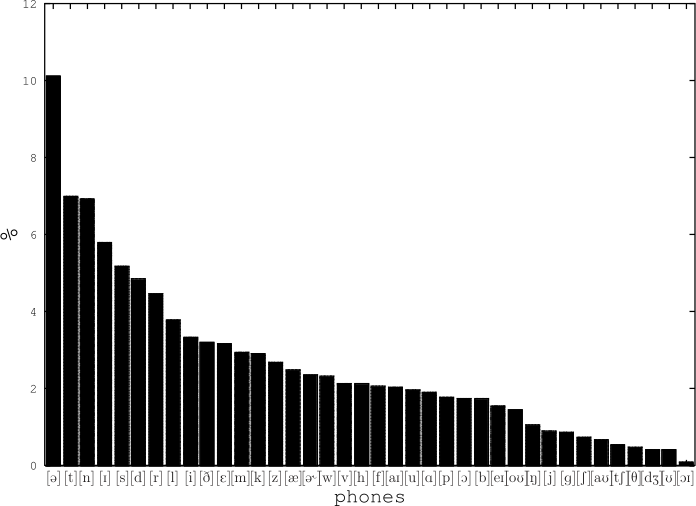
\includegraphics[width=\textwidth]{images/phones_hist_en.pdf}
}
\caption{Frequency of occurrence of English phones.}
\label{fig:phones_hist_en}
\end{figure}

If we had these relative frequencies, during one language evolution, like the previous ones derived for English, they could be used as a first approximation to determine the thresholds for assimilation and dissmilation processes. The phonemes cannot have, all of them, the same percentage-threshold, for the weakening of a phoneme, causing an assimilation process, could lead the target phoneme to an excessive relative frequency, and it would require this target phoneme to be capable of sustaining a higher frequency then the vanishing one. It is quite reasonable to consider that phonemes have distinct thresholds, what might be explained by their different acoustic and usage properties. It would be necessary to apprise and compare the features of phonemes, and also the way they are used and connected to build utterances.

According to \cite{zipf1949}, when a phoneme become so rare, with a relative frequency abnormally low, ``the phoneme then would become a distinctive and very characteristic part of every word in which it occurred''. In such situations, an accidental epenthesis might appear, like the strengthening of \textipa{[t]} into \textipa{[ts]} observed in the Old-High-German sound-shift in which a Germanic \textipa{[t]} shifted to a \textipa{[ts]} in the majority of positions, and it went even further in some cases to \textipa{[ss]}. Some examples in German, compared to the English counterpart, which preserved the \textipa{[t]}, are: \textit{zwei}, \textit{two}; \textit{zehn}, \textit{ten}; \textit{zug}, \textit{tug}; \textit{zahn}, \textit{tooth}; \textit{zeit}, \textit{time}.

Observing 12 languages, \cite{zipf1949} concludes that, with a few exceptions 
(the Spanish \textit{d} and \textit{t}, and the Hungarian \textit{b} and \textit{p}), 
the voiceless stops strongly outnumber their voiced counterparts and the relative frequencies 
of occurrence are amazingly similar. Considering that the voicing assimilation is a normal 
process found in many languages, it seems a quite astonishing result. It seems like other factors 
prevent this assimilation process from occurring. We could then consider the hypothesis that voiced 
stops have a lower threshold, and the assimilation process would force them to cross this threshold. 
In this situation, the assimilation would not move forward, and the voiceless stops are in a great number 
preserved.

The temporal nature of speech is evident. During an utterance, a speech context is built, and such a context is capable of influencing how speech is perceived. The perception of a initial sound of \textipa{[k]} or \textipa{[g]} is influenced by the following sounds, \textipa{[Is]} or \textipa{[Ift]}, for example, creating confusion and leading to false identifications (in the case of \textipa{[kIft]} or \textipa{[gIs]}) due to the existence of the words `gift' and `kiss'. The perception of what is currently being uttered both influences and is influenced by the perception of what comes later and what came previously. So, we might think of speech as a memory non-causal process.

Another aspect, as we observe the speech phenomena through time, is that, although we fight to achieve a segmental model of successive speech units, it has not been shown possible to split the speech continuum into a sequence of discrete elements, since the speech cues frequently overlap in time. The schematic problem of the overlap is shown in Figure \ref{fig:liberman}. The problem of overlap is less severe but still exists at word level. In normal speech, mainly in rapid speech, words run into each other. This phenomena is easy to perceive when we are listening to a foreign language and we can't tell when a word ends and another starts. It is not unusual to have speech errors due to wrong segmentation of words, what might be influenced by the context \citep{bondgarnes,cole1980}.

\begin{figure}[h!]
\centering
\includegraphics[width=0.45\textwidth]{images/liberman.png}
\caption{A schematic spectrogram for the word `bag' presenting the overlapping of acoustic cues. \citep{liberman1970}}
\label{fig:liberman}
\end{figure}  

There have been many ideas of how speech perception works and what are the basic units of it. It is still not clear how we segment speech as we perceive or whether we segment it at all. Various researchers advocate in favor of different approaches: \cite{klatt1979} arguments in favor of diphones; \cite{pisoni1982} in favor of phonemes, what seems to be the most accepted view in the literacy; \cite{fujimura1978} argues in favor of demisyllable; \cite{wickelgren1969} is in favor of context-sensitive allophones; and \cite{studdert1976} is in prol of using syllables as basic units. It seems reasonable to take the advantages of each approach and overcome each of their drawbacks, to take the problem under a multi-resolution point of view. It would, at a first glance, increase the complexity of the model.


The cues not only overlap one into another, but they also are different according to the various context they may appear. As presented by \cite{liberman1967}, the second-formant transition is responsible for determining what consonant the listener perceives. Figure \ref{fig:liberman2} presents some results for different transitional patterns for the second-formant.

\begin{figure}[h!]
\centering
\includegraphics[width=0.75\textwidth]{images/liberman2.png}
\caption{The second-formant starts at, or points to, the \textipa{/d/} locus. On (a), the syllables were perceived as \textipa{/b/}, \textipa{/d/} or \textipa{/g/}, depending on the final frequency level of the formant. On (b), all syllables were perceived as beginning with \textipa{/d/}. \citep{liberman1967}}
\label{fig:liberman2}
\end{figure} 


\chapter{Pronouncing Dictionary}
\epigraph{People are under the impression that dictionaries legislate language. What a dictionary does is keep track of usages over time.}{Steven Pinker}

%\begin{table}[htbp]
%\label{tbl:vowels_arpabet_ipa}
%\caption{Arpabet Symbols and their IPA equivalents : Vowels}
%\centering
%\begin{tabular}{|c|c|c|c|c|c|}
%\hline 
%Arpabet & IPA & Arpabet & IPA & Arpabet & IPA \\ 
%\hline  \hline
%AA & \textipa{[A]} & IH & \textipa{[I]} & AY & \textipa{[aI]} \\ 
%\hline 
%AE & \textipa{[\ae]} & IY & \textipa{[i]} & AW & \textipa{[aU]} \\ 
%\hline 
%AH0 & \textipa{[@]} & UH & \textipa{[U]} & EY & \textipa{[eI]} \\ 
%\hline 
%AH1 & \textipa{[2]} & UW & \textipa{[u]} & OW & \textipa{[oU]} \\ 
%\hline 
%AO & \textipa{[O]} & ER0 & \textipa{[@\textrhoticity]} & EH & \textipa{[E]} \\ 
%\hline 
%EH & \textipa{[E]} & ER1 & \textipa{[3\textrhoticity]} &  &  \\ 
%\hline 
%\end{tabular} 
%\end{table}
%
%
%
%
%\begin{table}[htbp]
%\label{tbl:vowels_arpabet_ipa}
%\caption{Arpabet Symbols (AB) and their IPA equivalents : Consonants}
%\centering
%\begin{tabular}{|c|c|c|c|c|c|c|c|c|c|c|c|}
%\hline 
%AB & IPA & AB & IPA & AB & IPA & AB & IPA & AB & IPA & AB & IPA  \\ 
%\hline  \hline
%\multicolumn{12}{|c|}{stops} \\
%\hline
%P & \textipa{[p]} & B & \textipa{[b]} & T & \textipa{[t]} & D & \textipa{[d]} & K & \textipa{[k]} & G & \textipa{[g]} \\
%\hline
%
%\multicolumn{12}{|c|}{affricates} \\
%\hline
%CH & \textipa{[tS]} & JH & \textipa{[dZ]} & & & & & & & & \\
%\hline
%
%\multicolumn{12}{|c|}{fricatives} \\
%\hline
%F & \textipa{[f]} & V & \textipa{[v]} & TH & \textipa{[T]} & DH & \textipa{[D]} & S & \textipa{[s]} & Z & \textipa{[z]} \\
%\hline
%SH & \textipa{[S]} & ZH & \textipa{[Z]} & HH & \textipa{[h]} & & & & & & \\
%\hline
%
%\multicolumn{12}{|c|}{nasals} \\
%\hline
%M & \textipa{[m]} & N & \textipa{[n]} & NG & \textipa{[N]} & & & & & & \\
%\hline
%
%\multicolumn{12}{|c|}{liquids} \\
%\hline
%L & \textipa{[l]} & R & \textipa{[r]} & & & & & & & & \\
%\hline
%
%\multicolumn{12}{|c|}{semivowels} \\
%\hline
%Y & \textipa{[j]} & W & \textipa{[w]} & Q & \textipa{[P]} & & & & & & \\
%\hline 
%\end{tabular} 
%\end{table}
%


%\newpage
Pronunciation dictionaries are lists of words or phrases with their
respective pronunciation transcribed into a phonetic alphabet.
The pronunciation of words may vary much in spontaneous speech,
and for that reason many dictionaries include some of the possible variations
found in spoken interactions. Pronunciation dictionaries usually reflect
one particular spoken accent, usually chosen as the most neutral 
among the various accents in a language. They are constructed by hand
or by a rule-based system. Pronunciation dictionaries are most used in
speech recognition system and synthesizers, and the usage of an appropriate
one may improve significantly the system performance \citep{lamel1996}.
Research efforts have been aiming to build pronouncing dictionaries that are 
automatically trained with real speech data and preliminary experiments
have shown the achievement of good results, eliciting higher recognition
rate systems \citep{fukada97}.

In order to acquire statistical information on speech pronunciation using
a text database, we may use a pronouncing dictionary to transcribe words
into a sequence of phones. A few tools are available nowadays to be used
in this purpose:
\begin{description}
\item[Moby Pronunciator II] contains 177,267 words with corresponding pronunciations
fully International Phonetic Alphabet coded. Stress or emphasis is also marked in the data.
It was createb by William Grady Ward and in 2007 has been placed into the public domain.
\item[TIMIT] corpus of read speech contains a total of 630 sentences spoken by
10 different speakers from 8 major dialect regions of the United States. The total
number of words in the corpus is only 659 words. The corpus has phonemically and lexically 
transcribed speech. It was created as a joint effort from  the Massachusetts
Institute of Technology, Stanford Research Institute, and Texas Instruments.
\item[ICSI Switchboard] is a corpus of several informal speech conversations, containing over
3 million words, recorded over the telephone. It includes a pronouncing lexicon with 71,100
entries using a modified Prolex phonetic alphabet.
\item[CMUdict] is a public domain dictionary created by Carnegie Mellon University. 
It contains 133,746 entries of English words mapping between its written form and their 
North American pronunciations.
\end{description}
These corpora cited above have been designed to provide data for
the creation of acoustic-phonetic knowledge and for the development and
evaluation of automatic speech recognition systems and speech synthesizers.

The present work aims into acquiring statistical knowledge of the patterns found in
the acoustic-phonetic behavior of the English language. To reach this sort of information
from textual data, we chose to use the Carnegie Mellon University Pronouncing Dictionary
(CMUdict) since it is available in public domain, is widely used and has many entries.
%a large number of
%entries.

\section[CMUdict]{The Carnegie Mellon University Pronouncing Dictionary}

The Carnegie Mellon University (CMU) Pronouncing Dictionary is a 
machine-readable pronunciation dictionary for North American English
created as public domain resource. It defines a mapping from English
words to their North American phonetic transcriptions. 
Those transcriptions are coded by the ARPAbet\footnote{
``Arpabet is a phonetic transcription code developed by the Advanced Research Projects Agency (ARPA) as a part of their Speech Understanding Project (1971--1976). It represents each phoneme of General American English with a distinct sequence of ASCII characters. Arpabet has been used in several speech synthesizers, like SAM for the Commodore 64, Say for the Amiga and TextAssist for the PC. It is also used in the CMU Pronouncing Dictionary''(Wikipedia).
} \citep{Shoup1988}, a phonetic transcription 
code developed by Advanced Research Projects Agency (ARPA).
``In November of 1971, the Information Processing Technology Office of the
Advanced Research Projects Agency of the Department of Defense (ARPA) 
initiated a five-year research and development program with the
objective of obtaining a breakthrough in speech understanding capability
that could then be used toward the development of practical man-machine
communication systems. (...) The objectives were to develop several
speech understanding systems that accept continuous speech from many 
cooperative speakers of a General American dialect'' \citep{klatt1977}.
It uses a set of 39 phones that represents the speech inventory of the 
General American English\footnote{
General American English, also known as Standard American English, is the standard
accent used by most of the American films, TV series, news, advertisements and radio
broadcasts. The area of eastern Nebraska, southern and central Iowa, and western Illinois
are considered to be the places where local accent is most similar to General American
\citep{labov2006atlas}.
}
It doesn't make any 
kind of surface reduction like flapping or reduced vowels, since
``predicting reduction requires knowledge of things outside the lexicon (the prosodic context, 
rate of speech, etc.)'' \citep{jurafsky2009speech}.
Instead, the vowels are marked by a number indicating the stress associated with them.
%: 0 (unstressed),
%1 (stressed), and 2 (secondary stress).


Tables \ref{tbl:vowels_arpabet_ipa} and \ref{tbl:consonants_arpabet_ipa} 
present the equivalence between IPA code and ARPAbet code.
The CMU Pronouncing Dictionary was chosen to be used since it 
is the pronouncing dictionary with the most number of words (contains over 133,000 entries) 
and it is open and free to use.
The CMU Pronouncing Dictionary is also commonly
used in many speech processing applications such as the 
Festival Speech Synthesis System and the CMU Sphinx speech recognition system.

The format used by the CMU Pronouncing Dictionary has mappings from words to their pronunciations
using the phone set given by a modified ARPAbet system (the difference is the stress marks used on vowels). 
The current phone set contains 39 phones
(not counting variations due to lexical stress) and 
the vowels may be marked by their lexical stress using the scale: 0 (no stress), 1 (primary stress)
and 2 (secondary stress). When alternate pronunciations exist for a given word, they are
marked by an index within parentheses. The first version of the dictionary was release on 16th of September 1993.
The version used was 0.7a, released on 19th February 2008.

\begin{table}[htbp]
\caption{Arpabet Symbols and their IPA equivalents : Vowels}
\centering
\begin{tabular}{|l|l|c|c|l|l|} \hline
 & & IPA Symbol & ARPAbet & Example & Transcription \\ \hline
\multirow{23}{*}{Vowels} & \multirow{4}{*}{Front} & \textipa{i} & IY & beat & B IY1 T \\
  &  & \textipa{I}   & IH & bit & B IH1 T \\ 
  &  & \textipa{E}   & EH & bet & B EH1 T \\
  &  & \textipa{\ae} & AE & fast & F AE1 S T \\ \cline{2-5}

  & \multirow{4}{*}{Back} & \textipa{A} & AA & father & F AA1 DH ER0 \\ 
  &  & \textipa{O} & AO & frost & F R AO1 S T \\
  &  & \textipa{U} & UH & book & B UH1 K \\
  &  & \textipa{u} & UW & boot & B UW1 T \\ \cline{2-5}

  & \multirow{2}{*}{Mid} & \textipa{@} & AX & discus & D IH1 S K AX0 S \\ % or  D IH1 S K AH0 S \\
  &  & \textipa{2} & AH & but & B AH1 T \\ \cline{2-5}

  & \multirow{5}{*}{Diphthongs} & \textipa{eI} & EY & bait & B EY1 T\\ 
  &  & \textipa{aI} & AY & my  & M AY1 \\
  &  & \textipa{aU} & AW & how & HH AW1 \\
  &  & \textipa{OI} & OY & boy & B OY1 \\
  &  & \textipa{oU} & OW & show & SH OW1 \\ \cline{2-5}
  
  & \multirow{8}{*}{R-colored} & \textipa{3\textrhoticity} & ER & her & HH ER0 \\
  &  & \textipa{@\textrhoticity} & AXR & father & F AA1 DH ER \\
  &  & \textipa{Er} & EH R & air & EH1 R \\
  &  & \textipa{Ur} & UH R & cure & K Y UH1 R \\
  &  & \textipa{Or} & AO R & more & M AO1 R \\
  &  & \textipa{Ar} & AA R & large & L AA1 R JH \\
  &  & \textipa{Ir} & IH R or IY R & ear & IY1 R \\
  &  & \textipa{aUr} & AW R & flower & F L AW1 R \\ \hline % or F L AW1 ER0 \\ \hline
\end{tabular}
\label{tbl:vowels_arpabet_ipa}
\end{table}  


%Phonetic reduction most often involves a centralization of the vowel, that is, a reduction in the amount of movement of the tongue in pronouncing the vowel, as with the characteristic change of many unstressed vowels at the ends of English words to something approaching schwa. 
% non reduced : AH1 : example, but (B AH1 T), sun (S AH1 N)
% reduced : AH0 = AX : example, sofa (S OW1 F AH0), alone (AH0 L OW1 N), discus (D IH1 S K AX0 S)
%


\begin{table}[htbp]
\caption{Arpabet Symbols and their IPA equivalents : Consonants}
\centering
\begin{tabular}{|l|l|c|c|l|l|} \hline
 & & IPA Symbol & ARPAbet & Example & Transcription \\ \hline
\multirow{6}{*}{Stops} & \multirow{3}{*}{Voiced} & \textipa{b} & B & bat & B AE1 T \\
 &  & \textipa{d} & D & deep & D IY1 P \\
 &  & \textipa{g} & G & go & G OW1 \\ \cline{2-5}
 &  \multirow{3}{*}{Unoiced} & \textipa{p} & P & pea & P IY1 \\
 &  & \textipa{t} & T & tea & T IY1 \\
 &  & \textipa{k} & K & kick & K IH1 K \\ \hline
 
 
\multirow{6}{*}{Fricatives} & \multirow{4}{*}{Voiced} & \textipa{v} & V & very & V EH1 R IY0 \\
 &  & \textipa{D} & DH & that & DH AE1 T \\
 &  & \textipa{z} & Z  & zebra & Z IY1 B R AH0 \\
 &  & \textipa{Z} & ZH & measure & M EH1 ZH ER0 \\ \cline{2-5}
 &  \multirow{4}{*}{Unoiced} & \textipa{f} & F & five & F AY1 V \\ 
 &  & \textipa{T} & TH & thing & TH IH1 NG \\
 &  & \textipa{s} & S  & say & S EY1 \\
 &  & \textipa{S} & SH & show & SH OW1 \\ \hline
 
\multicolumn{2}{|l|}{ \multirow{2}[4]{*}{Affricates} } & \textipa{tS} & CH & church & CH ER1 CH \\ 
\multicolumn{2}{|l|}{} & \textipa{dZ} & JH & just & JH AH1 S T \\ \hline
 
 
\multicolumn{2}{|l|}{ \multirow{3}[4]{*}{Nasals} } & \textipa{m} & M & mom & M AA1 M \\ 
\multicolumn{2}{|l|}{} & \textipa{n} & N  & noon & N UW1 N \\
\multicolumn{2}{|l|}{} & \textipa{N} & NX & sing & S IH1 NG \\ \hline
  
\multicolumn{2}{|l|}{ \multirow{3}[4]{*}{Liquids} } & \textipa{l} & L & late & L EY1 T \\ 
\multicolumn{2}{|l|}{} & \textipa{r} & R  & run & R AH1 N \\
\multicolumn{2}{|l|}{} & \textipa{R} & DX & wetter & W EH1 T ER0 \\ \hline

\multicolumn{2}{|l|}{ \multirow{2}[4]{*}{Others} } & \textipa{h} & HH & house & HH AW1 S \\ 
\multicolumn{2}{|l|}{} & \textipa{?} & Q  & glottal stop \\ \hline
  
\multicolumn{2}{|l|}{ \multirow{3}[4]{*}{Semivowels} } & \textipa{j} & Y  & yes & Y EH1 S\\ 
\multicolumn{2}{|l|}{} & \textipa{w} & W  & way & W EY1 \\ 
\multicolumn{2}{|l|}{} & \textipa{\*w} & WH  & when & WH EH1 N\\ \hline  

%\multirow{5}{*}{Nasals} & \multirow{3}{*}{Non vocalic} & \textipa{m} & M & mom \\ 
%  &  & \textipa{n} & N  & noon \\
%  &  & \textipa{N} & NX & sing \\ \cline{2-5}
%  & \multirow{2}{*}{Vocalic} & \textipa{m} & EM & some \\ 
%  &  & \textipa{n} & EN & son \\ \hline
  
% &  & \textipa{} &  &  \\
% &  & \textipa{} &  &  \\ 
\end{tabular}
\label{tbl:consonants_arpabet_ipa}
\end{table}





The analysis proposed consider words as isolated structures and for that reason poslexical
phonological rules are not taken in account. Various phonological changes that happen in
a continuous speech, such as flapping, vowel reduction, and various coarticulation effects that
happen as a postlexical phonological change are not considered, since we are not evaluating the
effects of neighbor words on a continuous speech. % Although we don't consider these changes,
%we believe that it will not alter the statistical results, since the same phonological changes
%also take places within the lexical structures.








\chapter{Language Statistics}\label{sec:lang_stat}
\epigraph{In trying to give an account of the statistical properties of language,
one is faced with the problem of having to find the common thread which would
show the many and multifarious forms of language statistics - embodied in scattered
papers written by linguists, philosophers, mathematicians, engineers, each using his 
own professional idiom - as belonging to one great whole: quantitative linguistics.}{Gustav Herdan (1966)}

% total from short-gutenber database
% n. types: 164,444
% n. tokens : 14,285,332
% 
% 
% found in CMU
% n. types : 46,094
% n. tokens: 13,481,254
%
% merriam-webster has more than 470,000 
% wikitionary 2,030,838 entries
If we agree to see language as a purpose driven stochastic event, 
it is important to view its statistics and observe how it is structured. 
We might stipulate that language is a usage driven process, 
the way it is used is shaped by its structures,
%the very fact of its usage is modeled according to way it is structured, 
and the way it is structured is dictated by its usage. 
We see language then as a dynamic process in a constant feedback loop.

To understand the statistical properties and build models of languages is a central task in understanding
how language works and create natural language processing systems. Traditionally, language has
been studied and modeled manually, describing each observation and building a language grammar from them.
With the recent availability of a massive amount of data, statistically trained models are an attractive
alternative. Probabilistic models of language are also fundamental in speech recognition systems to
resolve ambiguity situations, and might also be used in optical character recognition, handwriting recognition,
spelling correction, part-of-speech tagging, and machine translation.


``One striking clue to the importance of probabilities in language comes
from the wealth of frequency effects that pervade language representation, processing, and language change.
(...) Frequent words are recognized faster than infrequent words, and there is a bias toward interpreting 
ambiguous words in terms of their more frequent meanings. Frequent words lead leniting changes and 
are more prone to reduction in speech. Frequent combinations of phonemes and structures are perceived as
more grammatical, or well formed, than infrequent combinations. 
The relative frequency of derived words and their bases affects the morphological decomposability of complex words'' 
\citep{bod2003}.

It is important to understand how frequency affects language processes and how the various
aspects of the cognition processes are driven and self-organized by usage.  
Humans seem to track, record and exploit the occurrences of various kinds of events.
This might make it fundamental to understand the statistical properties of language
to better understand how a language works.
\cite{pierrehumbert2003} proposes that linguistics constraints are a result of statistical robust generalizations
that might be effectively learned, transmitted and exploited.
The symbolic concept of a phoneme is a probabilistic distribution over a continuous phonetic space.
The process of learning, recognition and classification of phonetic exemplars is a task
of adjusting the phonemic membership functions. Under this point o view, language is a probabilistic process.
Knowlegde of phonotatics involves knowledge of co-occurence probabilities of phonemes, and the well-formedness
of a string of phonemes is just a combined product of the contributions of its subparts.
``Such phonotactic probabilities are exploited in speech perception for segmentation,
and they affect well-formedness judgments, influence pronunciation, and
affect behavior in linguistic tasks such as creating blends'' \citep{bod2003}.

The effect and influence of probabilities on Language is present at different levels.
\cite{baayen2003} presented the influence of the frequency of occurrence at the morpheme level,
showing that the individual's choice among concurring affixes is strongly biased by the frequency
of occurrence of these affixes. At the word level, the processing and representation of words
is strongly influenced by lexical frequency and this behavior is independent of morphological
composition of words. This frequency effect is manifested in ambiguity resolution,
phoneme reduction, language change and speed of access \citep{bod2003}.
Individuals also track the co-occurrence of words, what influences speech comprehension 
and production. \cite{jurafsky2003} argues that more frequent word pairs have a shorter processing time and
may also suffer a phonetic reduction. Low-probability words (regarding the surroundings)
are more likely to receive a pitch accent. \cite{jurafsky2003} provide evidence that 
``people track the probabilities of syntactic structures'', what influences the processing time
of sentences and structures, and it is also involved in disambiguation.

``Language displays all the hallmarks of a probabilistic system. Categories
and well-formedness are gradient, and frequency effects are everywhere.
We believe all evidence points to a probabilistic language faculty.
Knowledge of language should be understood not as a minimal set of
categorical rules or constraints, but as a (possibly redundant) set of gradient 
rules, which may be characterized by a statistical distribution'' \citep{bod2003}.

As remarked by \cite{sedelow1966}, ``the study of patterns formed in the process of the
linguistic encoding of information, is of importance to any major research focusing upon
or dependent upon the production or analysis of language''. An increased interest on
the statistical and numerical counts of linguistics objects is perceived on Languages research,
where the \textit{quantitative} aspects have gained an important status. The use of 
computational resource and the availability of digital information has made the quantitative analysis 
task possible, what was hitherto unfeasible.

The quantitative analysis is also the basis of \textit{stylometrics} (quantitative stylistics)
which deals with the analysis from the standpoint of individual or functional style.
Style is regarded as a probabilistic concept by which selection
(choice), conscious or unconscious, is responsible for creating a style,
an emergent feature during the choice process in a universe of multiple
alternatives for expressing an idea \citep{tuldava2004}.
The analysis of emergent patterns in communication and the influence on the linguistic style 
used is analyzed by \cite{hancock2004} to investigate the truthful and deceptive
dyadic communication. The studies show that ``senders used more words overall,
increased references to others, and used more sense-based descriptions (e.g., seeing, touching) when lying as compared
to telling the truth. Receivers naïve to the deception manipulation produced more words and sense terms, and
asked more questions with shorter sentences when they were being lied to than when they were being told the truth''
\citep{hancock2004}.



The first remarkable study in the statistics of languages was done by George Kingsley Zipf, 
linguistic professor of Harvard, during the 1920s and 1930s. Zipf and his students performed many 
word count experiments and determined that there is a relationship between the word's frequency of 
appearance in texts and its rank, the product of them is roughly a constant. 
%That means, the most frequent word occurs twice as often as the second most frequent word; which occurs twice as often as the fourth most frequent word, and so forth. 
That means, the distribution follows a power law: $f(k;s,N) = C k^{-s}$, where $f$ stands for frequency, 
$C$ is a constant, $k$ is the word rank, $s$ the slope, the exponent characterizing the distribution, 
and $N$ is the number of elements in the set. Zipf's law is not, in fact, a law in the rigorous
sense, but an empirical observation that has an apparent robustness.

%As the number of occurrences cannot be a fractional number, we ought to find the constant $C$. 
The constant $C$ is a normalizing constant that might be found by calculating 
%Let's consider then 
the total number occurrences of all elements:
\begin{equation}
\sum_{k=1}^{N} f(k;s,N) = \sum_{n=1}^{N} C n^{-s} \textmd{ .}
\end{equation}
Normalizing the occurrences of each element ranked $k$ by the total of occurrences, leads us to
\begin{equation}
\label{eq:zipflaw}
f(k;s,N) = \frac{k^{-s}}{\sum_{n=1}^{N} n^{-s}} \textmd{ ,}
\end{equation}
that means, the constant $C$ is given by
\begin{equation}
C = \frac{1}{\sum_{n=1}^{N} n^{-s}} \textmd{ .}
\end{equation}

\begin{figure}[h!]
\centering
\includegraphics[width=0.75\textwidth]{images/zipf_pmf.pdf}
\caption{Zipf probability mass function for $N=10$ on a log-log scale for different values of $s$.}
\label{fig:zipf_pmf}
\end{figure} 

Zipf developed the idea of using an intrinsic linguistic or psychological reason to explain this phenomenon observed in the world of words. He named his theory the `Principle of Least Effort' to explain why frequently encountered words are chosen to be shorter in order to require a little mental and physical effort to recall them and utter/write them. According to \cite{weiss1998}, Zipf's law seems to hold regardless the language observed. ``Investigations with English, Latin, Greek, Dakota, Plains Cree, Nootka (an Eskimo language), speech of children at various ages, and some schizophrenic speech have all been seen to follow this law''\citep{weiss1998}.

A study by \cite{nowak2000}, on the evolutionary dynamics languages, aim to understand how the transition from 
non-syntactic communications, typically found among many animals, could lead to syntactic communication,
only found among humans. A model for the population dynamics of language evolution was proposed,
and the conclusions show that ``natural selection can only favour the emergence of syntax
if the number of required signals exceeds a threshold value'' \citep{nowak2000}. The emergence of syntax might be
responsible for Zipf's pattern that is observed in human communication.

Zipf's law\footnote{A cumulative distribution with a power-law form is said to follow a \emph{Zipf's law}
or a \emph{Pareto distribution}. Zipf's law usually is used in a context to refer the relation between frequency
of occurrence of an event relative to it's rank. Pareto's law is given in terms of the cumulative distribution (CDF),
i.e. the number of events larger than a certain value is given by an inverse power of that value. A Power
law is simply the probability distribution function (PDF) associated with the CDF given by Pareto's law.} 
is also observed in other phenomena, for example: the magnitude of earthquakes 
(it is common to have many small earthquakes, but big ones are rare) \citep{suzuki2005}; 
the population in cities (there are few megalopolises, but thousands of small cities) \citep{gabaix1999}; 
the distribution of total liabilities\footnote{Liability, in financial accounting, 
``is a present obligation of the enterprise arising from past events, the settlement of which 
is expected to result in an outflow from the enterprise of resources embodying economic benefits'' 
(definition of the International Accounting Standards Board, IASB).} of bankrupted firms in high 
debt range \citep{fujiwara2004}; the number of requests for web pages \citep{huberman2002}; etc.

In order to derive the statistics for the English language, data from the Gutenberg Project\footnote{The Gutenberg Project (\url{http://www.gutenberg.org/}) is the oldest digital library and was founded in 1971 by Michael S. Hart. It has over 33,000 items in its collection and are free because their copyright has expired.} database were collected. The top 100 most downloaded books were initially used as our analysis database. Perl scripting was used to read all 100 books, list the words and count their occurrences. The top 59 most frequent words in the database and their number of occurrence are listed below. Using this list, it is straightforward to create a log-log plot presenting the words' rank versus their frequencies of occurrence, which is shown in Figure \ref{fig:wordfrequency_en}.

\begin{tiny}
\begin{multicols}{4}
\begin{enumerate}
    \item the : 775911
	\item and : 471916
	\item of : 414499
	\item to : 350613
	\item a : 277321
	\item in : 226505
	\item i : 200689
	\item that : 173083
	\item he : 162183
	\item it : 145364
	\item was : 130804
	\item his : 129300
	\item you : 118473
	\item with : 114122
	\item is : 112640
	\item for : 107245
	\item as : 102009
	\item not : 96636
	\item be : 86896
	\item but : 81643
	\item had : 80327
	\item at : 76688
	\item her : 75761
	\item on : 75493
	\item my : 73879
	\item him : 72258
	\item have : 68463
	\item this : 67572
	\item all : 65960
	\item me : 64560
	\item by : 63944
	\item which : 63051
	\item she : 57839
	\item they : 57770
	\item from : 56128
	\item or : 52089
	\item so : 51617
	\item said : 50040
	\item no : 48930
	\item are : 45831
	\item one : 43822
	\item what : 41575
	\item them : 41320
	\item were : 40475
	\item will : 39733
	\item if : 38421
	\item there : 38209
	\item we : 37944
	\item when : 37385
	\item their : 36721
	\item who : 36109
	\item an : 35485
	\item your : 33401
	\item would : 32582
	\item do : 31225
	\item out : 30165
	\item then : 29682
	\item been : 29502
	\item up : 28860
	\item[] $\ldots$
\end{enumerate}
\end{multicols}
\end{tiny}

\begin{figure}[h!]
\centering
\includegraphics[width=0.75\textwidth]{images/wordfrequency_en.pdf}
\caption{Log-log plot of words rank versus frequency of occurrence (only the 1,000 first words are presented).}
\label{fig:wordfrequency_en}
\end{figure} 

In the analysis presented, all strings of letters separated by white spaces were considered words. The definition of word itself is, in certain aspects, dubious. It is considered as the smallest free form that can be uttered or written and carries a meaning. This is the concept introduced by \cite{bloomfield1926} but it is doubtful since some words are not minimal free forms, like \textit{the} and \textit{of}, which make no meaning by themselves. There are also those meanings that require two strings of letters to express themselves, like: \textit{stock market}, \textit{apple tree}, \textit{carbon dioxide}, \textit{electric guitar}, \textit{hot tub}, \textit{cotton candy}, \textit{dental floss}, \textit{hot dog}, among others. There are some words that are clearly compound ones, like: \textit{newspaper}, \textit{thumbnail}, \textit{copperhead}, \textit{eyelid}, \textit{bedroom}, etc.; and from the previous example, we see that there is a tendency of some two words becoming a compound word, for example, \textit{hot dog} it also written as \textit{hotdog}. In other languages, like German, it is even harder to settle the boundaries of words. In 1996, the German word \textit{Donaudampf\-schifffahrt\-selektrizitäten\-haupt\-betriebs\-werkbau\-unter\-beamten\-gesellschaft} (Association for subordinate officials of the head office management of the Danube steamboat electrical services) was added to the Guinness Book of World Records as the largest word in that language. But the longest word that is not created artificially seems to be \textit{Rindfleische\-tikettierungs\-über\-wachungs\-aufgaben\-über\-tragungs\-gesetz} (Cattle marking and beef labeling supervision duties delegation law).

Anyway, we are interested in language as a spoken means of communication, not a written one, 
although it is known that one influence the other. %(see section \ref{speech_written_interactions}). 
However we don't have a speech database and it would be hard and time consuming to create one, 
we adopted the Carnegie Mellon University (CMU) Pronouncing Dictionary to get the phonetic transcription 
of the words in our database. The CMU Dictionary is a public domain pronouncing dictionary for 
North American English that contains over 125,000 words and their transcriptions. 
It is used as the American lexicon for the Festival Speech Synthesis System and also for 
the CMU Sphinx speech recognition system. Our database extracted from the Gutenberg's books is 
made of 164,444 words (types) and 14,285,332 occurrences of such words (tokens). 
It is still small when compared to the number of entries of some American English dictionaries 
(Merriam-Webster has more than 470,000 entries), but it suffices for a first analysis. 
Unfortunately only 25\% of the words matched the words in the CMU Dictionary, 
some of them because of spelling differences, like the one in \textit{colour - color}, 
\textit{favour - favor} and \textit{neighbourhood - neighborhood}; 
other because they are old-English words, like \textit{thyself}, \textit{milady}, 
\textit{beheld} and \textit{picot}; and all the rest is attributed to misspelling, 
proper names, abbreviations, foreign words or even words that are really not part of 
the CMU Dictionary vocabulary.
% 119,026 out CMU
% 46,094 in CMU

Using the database, transcribed through the CMU Dictionary, it was possible to draw 
some conclusions from the phones usage in English. We present first the list of phones 
and their frequency of occurrence:
\begin{tiny}
\begin{multicols}{4}
\begin{enumerate}
    \item \textipa{@} : 44539 
	\item \textipa{t} : 33131 
	\item \textipa{n} : 31928 
	\item \textipa{I} : 28845 
	\item \textipa{s} : 21928 
	\item \textipa{d} : 20032 
	\item \textipa{r} : 18563 
	\item \textipa{i} : 16482 
	\item \textipa{l} : 15816 
	\item \textipa{E} : 13896 
	\item \textipa{m} : 13072 
	\item \textipa{3\textrhoticity} : 12640 
	\item \textipa{k} : 12308 
	\item \textipa{w} : 11107 
	\item \textipa{z} : 10744 
	\item \textipa{D} : 10720 
	\item \textipa{v} : 10407 
	\item \textipa{h} : 10009 
	\item \textipa{f} : 9391 
	\item \textipa{A} : 8744 
	\item \textipa{\ae} : 8635 
	\item \textipa{b} : 8390 
	\item \textipa{u} : 7972 
	\item \textipa{p} : 7501 
	\item \textipa{O} : 7429 
	\item \textipa{eI} : 6196 
	\item \textipa{aI} : 6148 
	\item \textipa{oW} : 5283 
	\item \textipa{S} : 4915 
	\item \textipa{N} : 4861 
	\item \textipa{g} : 3351 
	\item \textipa{tS} : 2501 
	\item \textipa{j} : 2462 
	\item \textipa{T} : 2309 
	\item \textipa{U} : 2276 
	\item \textipa{aU} : 2242 
	\item \textipa{dZ} : 2100 
	\item \textipa{OI} : 326 
	\item \textipa{Z} : 314 
\end{enumerate}
\end{multicols}
\end{tiny}
The data above are used to plot the frequency of occurrence of the phones against 
their rank, as seen in Figure \ref{fig:phonesfrequency_en}, shown in a log-log plot. 
We may observe that the data don't form a straight line, 
what could be expected, since we are dealing with a very small set and Zipf's law is
characteristic of a class of Large Number of Rare Events (LNRE) \citep{baayen2001}. 
%When we have a set holding a large number of low-probability elements, we expect to
%observe a proportional undersampled subset in any given sample.
Since the number of distinctive phones is quite small, we will observe a reasonably
well estimated phones' probabilities. As we move forward to larger units: bigrams, trigrams,
etc., we expect to increase the chances of observing a power law relation.

%%and we might conclude that they don't follow a Zipf's law-like curve. 
%As already pointed out by \cite{li1992}, ``Zipf's law is not a deep law in natural language 
%as one might first have thought. It is very much related to the particular representation one 
%chooses, i.e., rank as the independent variable.'' \cite{li1992} showed that random texts also 
%exhibit Zipf's law-like curves. 
\cite{li1992} argues that the pattern observed in Zipf's law has significant value
since it is a natural observation on random processes.
Even though, we observe that, as we analyze larger chunks of 
symbols, the relation between the frequency of occurrence of these chunks and their rank 
approximate progressively a Zipf's law (see Figure \ref{fig:simulate_chunks}).

\begin{figure}[h!]
\centering
\includegraphics[width=0.75\textwidth]{images/phonesfrequency_en.pdf}
\caption{Log-log plot of phones rank versus frequency of occurrence.}
\label{fig:phonesfrequency_en}
\end{figure} 


\begin{figure}[h!]
%\centering
\noindent\makebox[\textwidth]{%
\includegraphics[width=1.0\textwidth]{images/simulate_chunks.pdf} }
\caption{Log-log plot of the rank of chunks of different sizes versus their frequency of occurrence.}
\label{fig:simulate_chunks}
\end{figure}

Another way to see the Zipf's law is as a distribution of Pareto. The Pareto principle states that, for many events, most of the effects come from the minority of the causes.  This principle was named after the Italian economist Vilfredo Pareto. In 1906, he observed that 80\% of the land in Italy was owned by 20\% of the population. The phrase ``The $k$th most frequent word has $n$ occurrences'' may be stated, from the Pareto's perspective, as ``$k$ words occur $n$ or more times''. A Pareto plot is shown in Figure \ref{fig:phones_pareto}. It combines a bar chart displaying percentages of the English phones (categories) with a line graph showing cumulative percentages of these categories. We observe that the 8 first most frequent phones (\textipa{[@, t, n, s, I, r, d, l]}) account for half of all phones occurrences in the data. 
In turn, the Figure \ref{fig:phonesfrequencyocc_en} is a simple ordinary plot of the phones and their respective frequency of occurrence. 
%The last figure \ref{fig:phonescumulativeprobability_en} presents the cumulative distribution for the English phones. 


\begin{figure}[h!]
%\centering
\noindent\makebox[\textwidth]{%
\includegraphics[width=0.95\textwidth]{images/phones_pareto.pdf}
}
\caption{Pareto plot of the English phones.}
\label{fig:phones_pareto}
\end{figure} 





\begin{figure}[h!]
%\centering
\noindent\makebox[\textwidth]{%
\includegraphics[width=0.95\textwidth]{images/phonesfrequencyocc_en.pdf}
}
\caption{Frequency of occurrence of English phones.}
\label{fig:phonesfrequencyocc_en}
\end{figure} 

%\begin{figure}[h!]
%\centering
%\includegraphics[width=0.75\textwidth]{images/phonescumulativeprobability_en.pdf}
%\caption{Frequency of occurrence of English phones.}
%\label{fig:phonescumulativeprobability_en}
%\end{figure} 


%%%% mover este paragrafo para outro lugar!!!
One important quantity that might be obtained from a database is a measure of the information
being transmitted by a source using a given set of symbols. The notion of information
is dealt by the concept of entropy (what be will discussed in more details in another section)
and is usually measured in bits. The greater the entropy of a source, the greater is the 
uncertainty associated with its output and then it is also greater the amount of information encoded
in its messages.
The entropy of spoken English, calculated from the data above, gives 4.84 bits per phone.
%which is considerably higher compared to the entropy of written English,
The entropy of written English was estimated by \citep{schneier1996}, who found it
to be between 1.0 and 1.5 bits per letter. %\citep{schneier1996}, 
It was also estimated by \cite{shannon1951}, having found a value between 0.6 and 1.3 bits per letter,
%what was found by \cite{shannon1951} 
in a experiment where subjects were asked to predict
the next letter in a English text. 
The relative entropy, Kullback–Leibler divergence, of English 
phones compared to a uniform random distribution is 0.45 bits.
%0.48 bits.

Zipf believed that the change in frequency was responsible for triggering the 
mechanism of combination. He supposes that the frequency of occurrence of a
lower level unity is proportional to the number of higher level structures 
it will appear on. The low specificity of a lower level unit
makes it more suitable for been used in making higher level structures.
Figure \ref{fig:phones_num_words_freq_occ} presents the relationship
between the frequency of occurrence of English phones and the number
of English words they appear on. 

\begin{figure}[h!]
\centering
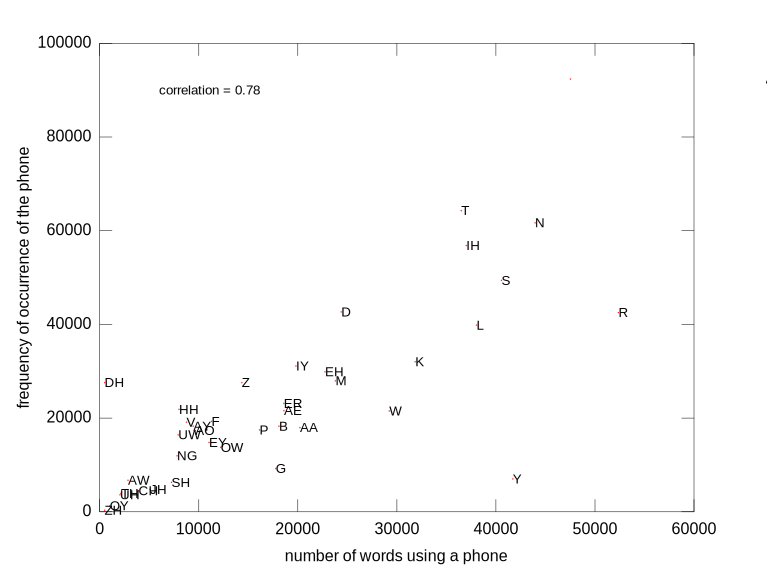
\includegraphics[width=0.65\textwidth]{images/phones_num_words_freq_occ.pdf}
\caption{Relation between the frequency of occurrence of phones and the number of words they appear.}
\label{fig:phones_num_words_freq_occ}
\end{figure} 

The distribution of the occurrence of a given phone is not uniform across the rank of words in a language. 
Nor can't we conclude that the high frequency of certain phones is due to the high frequency of the words they appear. 
Figure \ref{fig:proboccwordsphone} shows the probability of occurrence of phones across the rank of words. 
We might observe that the probability of occurrence of a given phone is greater in rare words then in usual ones.
%against what we could intuitively conclude without an analysis of the data.
Since high rank words are longer, the probability of occurring any phone is greater than on low rank words.

\begin{figure*}[p]
  \centering 
  %\captionsetup[subfigure]{margin=10pt,singlelinecheck=false}
  \begin{tabular}{cc}
  \subfloat[Probability of occurrence of \textipa{[@]} in words versus words rank.]{\label{fig:proboccwordsphone_AH}\includegraphics[width=0.45\textwidth]{images/proboccwordsphone_AH.pdf}} &
  \subfloat[Probability of occurrence of \textipa{[t]} in words versus words rank.]{\label{fig:proboccwordsphone_T}\includegraphics[width=0.45\textwidth]{images/proboccwordsphone_T.pdf}} \\
  \subfloat[Probability of occurrence of \textipa{[n]} in words versus words rank.]{\label{fig:proboccwordsphone_N}\includegraphics[width=0.45\textwidth]{images/proboccwordsphone_N.pdf}} &
  \subfloat[Probability of occurrence of \textipa{[U]} in words versus words rank.]{\label{fig:proboccwordsphone_UH}\includegraphics[width=0.45\textwidth]{images/proboccwordsphone_UH.pdf}} \\
  \subfloat[Probability of occurrence of \textipa{[OI]} in words versus words rank.]{\label{fig:proboccwordsphone_OY}\includegraphics[width=0.45\textwidth]{images/proboccwordsphone_OY.pdf}} & 
  \subfloat[Probability of occurrence of \textipa{[Z]} in words versus words rank.]{\label{fig:proboccwordsphone_ZH}\includegraphics[width=0.45\textwidth]{images/proboccwordsphone_ZH.pdf}} 
  \end{tabular}
  \caption{Probability of occurrence of certain phones in words across the rank of words.}
  \label{fig:proboccwordsphone}
\end{figure*}

Analyzing the sound systems of human languages, we conclude that they show remarkable regularities. Although humans are able to pronounce and perceive a great variety of speech sounds, languages use only a subset of them. Under another perspective, the categories created by languages, in order to achieve communication, form a small subset of possible categories of speech sounds that have a certain regularity across languages. Those regularities might be explained by innate human cognitive capacities or by functional constraints of communication. Such constraints would be created by the requirement of language to be a robust learnable means of communication, which would be responsible for the existence of redundancy, predictability, distinguishability and the usage of sounds of easy understandability and repeatability.

In the analysis of 451 languages of the world made by \cite{maddieson1884} using the UPSID (the UCLA Phonological Segment Inventory Database), 921 different speech sounds are found. As shown in Figure \ref{fig:language_segments_hist}, most of the languages (66.3\%) have a repertoire of 20 to 37 speech sounds. 
%The maximal number of elements used is 141 in !X\~u; and the minimal is 11 in Rotokas and Pirah\~a. 
%That means, 
In each language, we use only a subset of all the speech sounds available (using as a reference the UPSID and the 919 phones on this database, 
a language typical uses between 1.2\% and 15.3\% of the available speech sounds). Analyzing the subsets used in each language, we present bellow 
a list of the 20 most frequent consonants and the 10 most frequent vowels (see tables \ref{tbl:consonants_most_freq} and \ref{tbl:vowels_most_freq}).


\begin{table}[h]
\caption{List of the 20 most frequent consonants in UPSID.}
\label{tbl:consonants_most_freq}
\begin{tabular}{|c|c|c|c|c|c|c|c|c|}
\hline consonant 		& \textipa{m} & \textipa{k} & \textipa{j} & \textipa{p} & \textipa{w} & \textipa{b} & \textipa{h} & \textipa{g} \\ 
\hline n. of languages	& 425 & 403 & 378 & 375 & 332 & 287 & 279 & 253 \\ 
\hline frequency 		& 94.2 & 89.4 & 83.8 & 83.2 & 73.6 & 63.6 & 61.9 & 56.1 \\ 
\hline 
\end{tabular} 

\begin{tabular}{|c|c|c|c|c|c|c|c|c|}
\hline consonant 		& \textipa{N} & \textipa{P} & \textipa{n} & \textipa{s} & \textipa{tS} & \textipa{S} & \textipa{t} & \textipa{f} \\ 
\hline n. of languages	& 237 & 216 & 202 & 196 & 188 & 187 & 181 & 180 \\ 
\hline frequency 		& 52.6 & 47.9 & 44.8 & 43.5 & 41.7 & 41.5 & 40.1 & 39.9 \\ 
\hline 
\end{tabular} 

\begin{tabular}{|c|c|c|c|c|}
\hline consonant 		& \textipa{l} & \textipa{\|[n} & \textipa{\|[t} & \textipa{\textltailn } \\ 
\hline n. of languages	& 174 & 160 & 152 & 141 \\ 
\hline frequency 		& 38.6 & 35.5 & 33.7 & 31.3 \\ 
\hline 
\end{tabular} 
\end{table}


\begin{table}[h]
\caption{List of the 10 most frequent vowels in UPSID.}
\label{tbl:vowels_most_freq}
\begin{tabular}{|c|c|c|c|c|c|c|c|c|c|c|}
\hline consonant 		& \textipa{i} & \textipa{a} & \textipa{u} & \textipa{E} & \textipa{o/O} & \textipa{e/E} & \textipa{O} & \textipa{o} & \textipa{e} & \textipa{~a} \\ 
\hline n. of languages	& 393 & 392 & 369 & 186 & 181 & 169 & 162 & 131 & 124 & 83 \\ 
\hline frequency 		& 87.1 & 86.9 & 81.8 & 41.2 & 40.1 & 37.5 & 35.9 & 29.0 & 27.5 & 18.4 \\ 
\hline 
\end{tabular} 
\end{table}

Comparing tables \ref{tbl:consonants_most_freq} and \ref{tbl:vowels_most_freq}, we observe that the most frequent vowels are not so frequent across languages in comparison to the most frequent consonants. In the UPSID, there are 180 vowels, 16 glides\footnote{Glide or semivowel contrast with vowels by being non-syllabic, they functions as the syllable boundary rather than nucleus. In our analysis we will consider only the following as semivowels: palatal approximant, labial-palatal approximant, velar approximant, labial-velar approximant, and their possible variations.\citep{martinezceldran2004}} and 725 consonants, which strongly outnumber the others. The languages in UPSID present from 6 to 117 consonants (and glides), averaging 22.7 and from 3 to 28 vowels, averaging 8.1. The ratio consonant to vowel ranged from 0.69 to 15.33, averaging about 3.38. On average, languages present three times as many consonants as vowels. Considering that the database with 451 languages has in its inventory 652 consonants and 269 vowels, we see that across the languages, the number of vowels used corresponds from 0.9\% to 17.9\% (averaging 3.0\%) of the possible vowels; and the number of consonants used goes from 0.9\% to 14.6\% (averaging 3.5\%) of the consonants in the database. We might then conclude that the segments are chosen proportionally among all the possibilities, there is no tendency in choosing consonant over vowels, or the other way around. Analyzing these results and those on tables \ref{tbl:consonants_most_freq} and \ref{tbl:vowels_most_freq}, we conclude that there is some sort of stronger constraint on consonants that push some of them to become more frequent across languages. A constraint of this kind also exists for vowels, but it is much weaker. We also observe that, in general, languages use a speech repertoire where the number of consonants is greater than the number of vowels. There are only 14 languages (Kashmiri, Bruu, Dan, Klao, Kaingang, Apinaye, Barasano, Yagua, Cubeo, Japreria, Panare, Andoke, Maxakali, Vanimo) in which the number of vowels is greater or equal to the number of consonants. There are 427 speech sounds that are present in only one language. The group of sounds that appear in 10 or fewer of the 451 languages in the database sum up more that 80\% of all 919 sounds in the database.


%180 vowels
%palatal approximant : 5
%labial-palatal approximant : 1
%velar approximant : 6
%labial-velar approximant : 4

% min(numVowels) =  3
% max(numVowels) =  28
% mean(numVowels) =  8.0532

% min(numConsonants) =  6
% max(numConsonants) = 117
% mean(numConsonants) =  22.663

% ratio = numConsonants./numVowels
% min(ratio) =  0.68750
% max(ratio) =  15.333
% mean(ratio) =  3.3798


Figure \ref{fig:freqidx_nsegs_upsid} presents the relationship observed across languages of the 
usage of frequent or rare segments with the number of segments used in that language. 
In order to do so, a frequency index is proposed by \cite{reetz2010}. 
This index is the average of the segment frequencies of the segments in a language. 
Each segment in the UPSID has a segment frequency that is the number of languages that contain 
a specific segment divided by the number of languages in UPSID. 
Each language has a certain segment-repertoire. The frequency index of a language is calculated 
as the average of the frequency index of all segments in a language repertoire. 
``If a language has only few segments, it is likely that these are rather common in the languages 
in UPSID. On the other hand, a language with many segments will also have many segments that are 
uncommon in the UPSID database''\citep{reetz2010}.

\begin{figure}[h!]
\centering
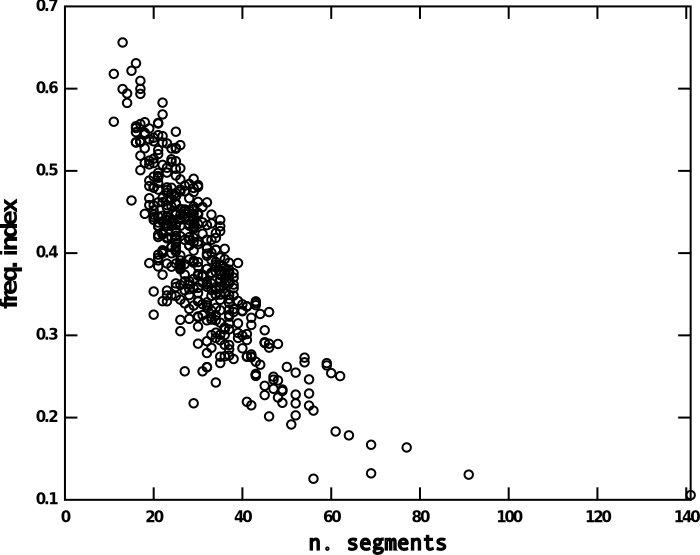
\includegraphics[width=0.65\textwidth]{images/freqidx_nsegs_upsid.pdf}
\caption{Relation between the frequency index and the number of phones in a language. (Data from UPSID)}
\label{fig:freqidx_nsegs_upsid}
\end{figure} 

%To understand how languages are structured, it is also important to 
%observe how categories emerge and how they are used. 
Using the UPSID database, we might find what speech segments co-occurs with each other in
different languages. When addressing the UPSID database, we shall use the term \emph{co-occurrence}  
to make reference to phones that occur in the same inventory. This remark is important in order to avoid
a possible confusion with the usual meaning of \emph{co-occurrence}, that is used to
assign phones that are neighbours in an utterance.  
%At a first glance, we might take on the co-occurrence of speech segments. Using the UPSID database 
We may find what are the most frequent co-occurring segment for another given segment 
(some results are in Figure \ref{fig:cooccurrence} and Table \ref{tbl:cooccurrence}). 
We notice that there is a large number of co-occurring segments for each one taken as a reference. 
The most frequent segments across languages have a great number of co-occurring segments, 
which represent approximately from 30\% to 60\% of all segments in UPSID. On the other hand, 
the most infrequent phones in the database have just a few co-occurring segments, around 3\%. 
Observing the graphics in Figure \ref{fig:cooccurrence}, we see that, for each reference segment, 
the co-occurring ones has a rapidly decreasing frequency of co-occurrence, what is expected from a random distribution. 
The high co-occurrence of certain pairs, in some cases, might be explained by the features they share. 
As an example, if we consider the bilabial consonants, we see that, as we take one as reference, 
the others appear in the top-10 list, showing a strong adhesion of one bilabial consonant to another. 
Observing now the voiced alveolar sibilant fricative \textipa{[z]}, its voiceless counterpart always appear, 
but doing the other way around analysis, taking \textipa{[s]} as a reference, its voiced counterpart \textipa{[z]} 
has a relative frequency of co-occurrence of 31.6\%, figuring as the 29th in the list. 
Analyzing other pairs like \textipa{[t]}-\textipa{[d]}, \textipa{[k]}-\textipa{[g]} and \textipa{[p]}-\textipa{[b]}, 
it seems that the existence of the voiced counterpart subjects the existence of the voiceless much more 
emphatically than the other way around.


\begin{figure*}[p]
  \centering 
  \captionsetup[subfigure]{margin=10pt,singlelinecheck=false,font={scriptsize,sf}}
  \subfloat[This graph presents the co-occurrence frequency for phones in relation to \textipa{[@]}. The phone \textipa{[k]} has a frequency of 96.0\%. \textipa{[m]} follows with 94.7\% and \textipa{[p]} with 90.7\%. 39.8\% of the phones in UPSID are co-occurring with the phone \textipa{[@]}.]{\label{fig:cooccurrence_01}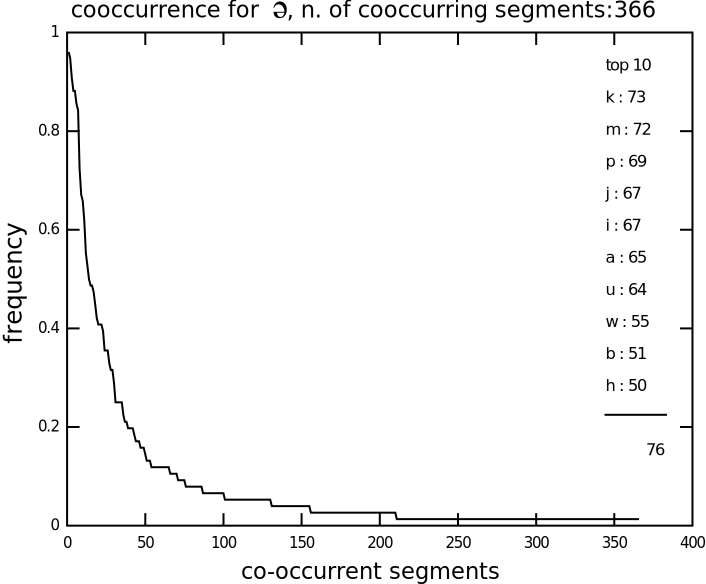
\includegraphics[width=0.45\textwidth]{images/cooccurrence_01.pdf}}                
  \subfloat[This graph presents the co-occurrence frequency for phones in relation to \textipa{[t]}. The phone \textipa{[k]} has a frequency of 96.1\%. \textipa{[m]} follows with 93.3\% and \textipa{[a]} with 91.2\%. 55.6\% of the phones in UPSID are co-occurring with the phone \textipa{[t]}.]{\label{fig:cooccurrence_02}\includegraphics[width=0.45\textwidth]{images/cooccurrence_02.pdf}} \\
  \subfloat[This graph presents the co-occurrence frequency for phones in relation to \textipa{[n]}. The phone \textipa{[m]} has a frequency of 99.0\%. \textipa{[a]} follows with 89.6\% and \textipa{[j]} with 89.1\%. 60.5\% of the phones in UPSID are co-occurring with the phone \textipa{[n]}.]{\label{fig:cooccurrence_03}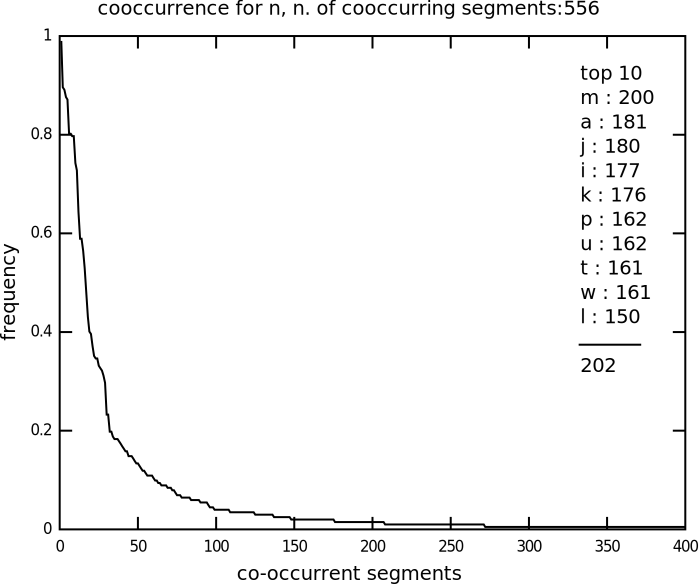
\includegraphics[width=0.45\textwidth]{images/cooccurrence_03.pdf}}
  \subfloat[This graph presents the co-occurrence frequency for phones in relation to \textipa{[l]}. The phone \textipa{[m]} has a frequency of 97.3\%. \textipa{[j]} follows with 91.9\% and \textipa{[k]} with 86.5\%. 38.8\% of the phones in UPSID are co-occurring with the phone \textipa{[l]}.]{\label{fig:cooccurrence_04}\includegraphics[width=0.45\textwidth]{images/cooccurrence_04.pdf}} \\
  \subfloat[This graph presents the co-occurrence frequency for phones in relation to \textipa{[s]}. The phone \textipa{[m]} has a frequency of 95.4\%. \textipa{[j]} follows with 89.3\% and \textipa{[a]} with 88.3\%. 62.0\% of the phones in UPSID are co-occurring with the phone \textipa{[s]}.]{\label{fig:cooccurrence_05}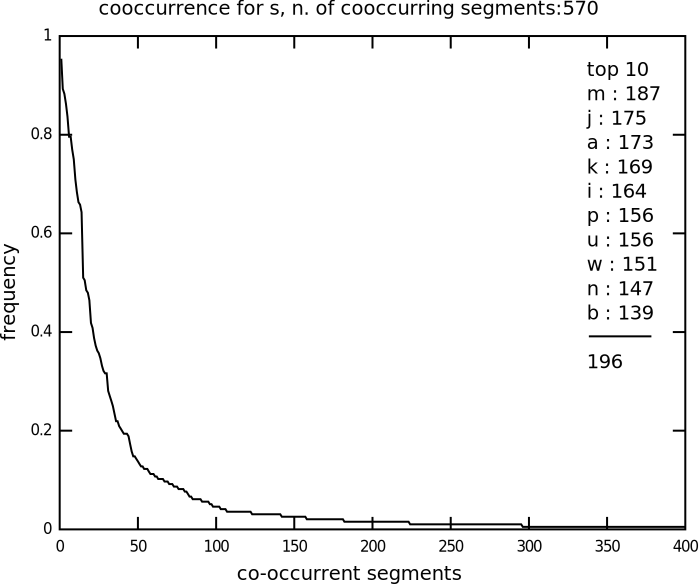
\includegraphics[width=0.45\textwidth]{images/cooccurrence_05.pdf}} 
  \subfloat[This graph presents the co-occurrence frequency for phones in relation to \textipa{[z]}. The phone \textipa{[s]} has a frequency of 100\%. \textipa{[m]} follows with 98.4\% and \textipa{[j]} with 93.5\%. 40.4\% of the phones in UPSID are co-occurring with the phone \textipa{[z]}.]{\label{fig:cooccurrence_06}\includegraphics[width=0.45\textwidth]{images/cooccurrence_06.pdf}} 
  \caption{The frequency co-occurrence plots above are derived from the UPSID.}
  \label{fig:cooccurrence}
\end{figure*}


\begin{table}[h]
\caption{List of phones and their top 10 co-occurring pairs with their relative frequency of occurrence (data from UPSID).}
\label{tbl:cooccurrence}
\begin{scriptsize}
\begin{tabular}{|c||c|c|c|c|c|c|c|c|c|c|c|}
\hline 
phone & \multicolumn{10}{|c|}{co-occurring phone with their respective relative frequency (\%)} \\  
\hline 
\textipa{@} & \textipa{k} : 96.1 & \textipa{m} : 94.7 & \textipa{p} : 90.8 & \textipa{j} : 88.2 & \textipa{i} : 88.2 & \textipa{a} : 85.5 & \textipa{u} : 84.2 & \textipa{w} : 72.4 & \textipa{b} : 67.1 & \textipa{h} : 65.8 \\ \hline
\textipa{t} & \textipa{k} : 96.1 & \textipa{m} : 93.4 & \textipa{a} : 91.2 & \textipa{p} : 90.1 & \textipa{n} : 89.0 & \textipa{i} : 87.3 & \textipa{j} : 85.6 & \textipa{w} : 80.7 & \textipa{u} : 80.1 & \textipa{s} : 71.3 \\ \hline
\textipa{n} & \textipa{m} : 99.0 & \textipa{a} : 89.6 & \textipa{j} : 89.1 & \textipa{i} : 87.6 & \textipa{k} : 87.1 & \textipa{p} : 80.2 & \textipa{u} : 80.2 & \textipa{t} : 79.7 & \textipa{w} : 79.7 & \textipa{l} : 74.3 \\ \hline
\textipa{I} & \textipa{m} : 97.3 & \textipa{j} : 91.9 & \textipa{k} : 86.5 & \textipa{a} : 83.8 & \textipa{p} : 83.8 & \textipa{U} : 74.3 & \textipa{w} : 71.6 & \textipa{b} : 66.2 & \textipa{g} : 64.9 & \textipa{N} : 63.5 \\ \hline
\textipa{s} & \textipa{m} : 95.4 & \textipa{j} : 89.3 & \textipa{a} : 88.3 & \textipa{k} : 86.2 & \textipa{i} : 83.7 & \textipa{p} : 79.6 & \textipa{u} : 79.6 & \textipa{w} : 77.0 & \textipa{n} : 75.0 & \textipa{b} : 70.9 \\ \hline
\textipa{z} & \textipa{s} : 100.0 & \textipa{m} : 98.4 & \textipa{j} : 93.5 & \textipa{k} : 91.9 & \textipa{b} : 90.3 & \textipa{g} : 90.3 & \textipa{p} : 82.3 & \textipa{i} : 80.6 & \textipa{u} : 80.6 & \textipa{a} : 80.6 \\ \hline
\textipa{d} & \textipa{b} : 96.7 & \textipa{m} : 94.2 & \textipa{i} : 91.7 & \textipa{a} : 90.8 & \textipa{j} : 90.0 & \textipa{n} : 89.2 & \textipa{g} : 87.5 & \textipa{u} : 86.7 & \textipa{t} : 85.8 & \textipa{k} : 84.2 \\ \hline
\textipa{l} & \textipa{m} : 98.9 & \textipa{j} : 89.1 & \textipa{k} : 86.8 & \textipa{n} : 86.2 & \textipa{a} : 86.2 & \textipa{i} : 85.6 & \textipa{p} : 81.0 & \textipa{w} : 79.9 & \textipa{u} : 79.9 & \textipa{s} : 72.4 \\ \hline
\textipa{i} & \textipa{m} : 93.9 & \textipa{u} : 91.6 & \textipa{k} : 89.6 & \textipa{a} : 89.1 & \textipa{p} : 82.7 & \textipa{j} : 82.7 & \textipa{w} : 73.8 & \textipa{b} : 65.1 & \textipa{h} : 62.6 & \textipa{g} : 57.5 \\ \hline
\textipa{\|[d} & \textipa{b} : 97.5 & \textipa{m} : 96.2 & \textipa{g} : 93.8 & \textipa{j} : 88.8 & \textipa{k} : 85.0 & \textipa{\|[t} : 83.8 & \textipa{i} : 80.0 & \textipa{p} : 76.2 & \textipa{u} : 72.5 & \textipa{a} : 70.0 \\ \hline
\textipa{m} & \textipa{k} : 89.2 & \textipa{i} : 86.8 & \textipa{a} : 86.6 & \textipa{j} : 85.2 & \textipa{p} : 82.6 & \textipa{u} : 81.6 & \textipa{w} : 74.1 & \textipa{b} : 64.2 & \textipa{h} : 61.6 & \textipa{g} : 56.7 \\ \hline
\textipa{n} & \textipa{m} : 99.0 & \textipa{a} : 89.6 & \textipa{j} : 89.1 & \textipa{i} : 87.6 & \textipa{k} : 87.1 & \textipa{p} : 80.2 & \textipa{u} : 80.2 & \textipa{t} : 79.7 & \textipa{w} : 79.7 & \textipa{l} : 74.3 \\ \hline
\textipa{k} & \textipa{m} : 94.0 & \textipa{p} : 91.3 & \textipa{i} : 87.3 & \textipa{a} : 86.6 & \textipa{j} : 83.4 & \textipa{u} : 82.1 & \textipa{w} : 73.2 & \textipa{b} : 62.8 & \textipa{h} : 61.0 & \textipa{g} : 54.1 \\ \hline
\textipa{g} & \textipa{b} : 96.4 & \textipa{m} : 95.3 & \textipa{i} : 89.3 & \textipa{j} : 87.4 & \textipa{k} : 86.2 & \textipa{u} : 84.2 & \textipa{a} : 83.0 & \textipa{p} : 76.7 & \textipa{w} : 72.3 & \textipa{h} : 63.6 \\ \hline
\textipa{p} & \textipa{k} : 98.1 & \textipa{m} : 93.6 & \textipa{a} : 87.2 & \textipa{i} : 86.7 & \textipa{j} : 82.9 & \textipa{u} : 81.3 & \textipa{w} : 71.7 & \textipa{b} : 60.5 & \textipa{h} : 60.3 & \textipa{N} : 54.4 \\ \hline
\textipa{b} & \textipa{m} : 95.1 & \textipa{i} : 89.2 & \textipa{k} : 88.2 & \textipa{j} : 86.8 & \textipa{g} : 85.0 & \textipa{u} : 84.3 & \textipa{a} : 84.3 & \textipa{p} : 79.1 & \textipa{w} : 72.5 & \textipa{h} : 65.9 \\ \hline
\textipa{S} & \textipa{m} : 94.7 & \textipa{j} : 91.4 & \textipa{k} : 88.8 & \textipa{i} : 84.0 & \textipa{a} : 82.9 & \textipa{p} : 80.2 & \textipa{u} : 78.1 & \textipa{w} : 74.3 & \textipa{h} : 73.3 & \textipa{b} : 68.4 \\ \hline
\textipa{Z} & \textipa{S} : 95.1 & \textipa{m} : 95.1 & \textipa{j} : 90.2 & \textipa{k} : 90.2 & \textipa{b} : 82.0 & \textipa{g} : 80.3 & \textipa{i} : 78.7 & \textipa{p} : 78.7 & \textipa{u} : 77.0 & \textipa{a} : 70.5 \\ \hline
\end{tabular} 
\end{scriptsize}
\end{table}


%@ : k 96.1   m 94.7   p 90.8   j 88.2   i 88.2   a 85.5   u 84.2   w 72.4   b 67.1   h 65.8
%t : k 96.1   m 93.4   a 91.2   p 90.1   n 89.0   i 87.3   j 85.6   w 80.7   u 80.1   s 71.3   
%n : m 99.0   a 89.6   j 89.1   i 87.6   k 87.1   p 80.2   u 80.2   t 79.7   w 79.7   l 74.3   
%I : m 97.3   j 91.9   k 86.5   a 83.8   p 83.8   U 74.3   w 71.6   b 66.2   g 64.9   N 63.5   
%s : m 95.4   j 89.3   a 88.3   k 86.2   i 83.7   p 79.6   u 79.6   w 77.0   n 75.0   b 70.9   
%z : s 100.0   m 98.4   j 93.5   k 91.9   b 90.3   g 90.3   p 82.3   i 80.6   u 80.6   a 80.6   
%d : b 96.7   m 94.2   i 91.7   a 90.8   j 90.0   n 89.2   g 87.5   u 86.7   t 85.8   k 84.2   
%l : m 98.9   j 89.1   k 86.8   n 86.2   a 86.2   i 85.6   p 81.0   w 79.9   u 79.9   s 72.4   
%i : m 93.9   u 91.6   k 89.6   a 89.1   p 82.7   j 82.7   w 73.8   b 65.1   h 62.6   g 57.5   
%dD : b 97.5   m 96.2   g 93.8   j 88.8   k 85.0   tD 83.8   i 80.0   p 76.2   u 72.5   a 70.0   
%m : k 89.2   i 86.8   a 86.6   j 85.2   p 82.6   u 81.6   w 74.1   b 64.2   h 61.6   g 56.7   
%n : m 99.0   a 89.6   j 89.1   i 87.6   k 87.1   p 80.2   u 80.2   t 79.7   w 79.7   l 74.3   
%k : m 94.0   p 91.3   i 87.3   a 86.6   j 83.4   u 82.1   w 73.2   b 62.8   h 61.0   g 54.1   
%g : b 96.4   m 95.3   i 89.3   j 87.4   k 86.2   u 84.2   a 83.0   p 76.7   w 72.3   h 63.6   
%p : k 98.1   m 93.6   a 87.2   i 86.7   j 82.9   u 81.3   w 71.7   b 60.5   h 60.3   N 54.4   
%b : m 95.1   i 89.2   k 88.2   j 86.8   g 85.0   u 84.3   a 84.3   p 79.1   w 72.5   h 65.9   
%S : m 94.7   j 91.4   k 88.8   i 84.0   a 82.9   p 80.2   u 78.1   w 74.3   h 73.3   b 68.4   
%Z : S 95.1   m 95.1   j 90.2   k 90.2   b 82.0   g 80.3   i 78.7   p 78.7   u 77.0   a 70.5 



If we believe that speech symbols repertoires are not chosen randomly, 
we might wonder what guides the choices of a repertoire. 
Not only the way those symbols are arranged, but also the way they are used (combined) 
is important in the process of understanding choices. 
Using the Gutenberg's database transcribed with the CMU pronouncing dictionary, as described above, we might get information 
on phone clusters frequency of occurrence (see also Figure \ref{fig:diphonesfrequency_en}):

\begin{tiny}
\begin{multicols}{4}
\begin{enumerate}
    \item \textipa{@n} : 1296408
    \item \textipa{D@} : 785354
    \item \textipa{nd} : 784028
    \item \textipa{st} : 651129
    \item \textipa{@v} : 489267
    \item \textipa{Or} : 472069
    \item \textipa{In} : 470069
    \item \textipa{tu} : 425544
    \item \textipa{t@} : 420825
    \item \textipa{IN} : 387096
    \item \textipa{Iz} : 380357
    \item \textipa{@l} : 372847
    \item \textipa{En} : 349905
    \item \textipa{nt} : 337193
    \item \textipa{\ae t} : 284460
    \item \textipa{wI} : 282526
    \item \textipa{@t} : 265396
    \item \textipa{Er} : 264293
    \item \textipa{r@} : 261447
    \item \textipa{It} : 260544
    \item \textipa{@s} : 246996
    \item \textipa{ju} : 245715
    \item \textipa{h\ae} : 237724
    \item \textipa{hI} : 237490
    \item \textipa{@m} : 233793
    \item \textipa{ri} : 219997
    \item \textipa{li} : 219652
    \item \textipa{An} : 213755
    \item \textipa{\ae n} : 213169
    \item \textipa{s@} : 210385
    \item \textipa{Is} : 208619
    \item \textipa{D\ae} : 194602
    \item \textipa{@f} : 193570
    \item \textipa{Ar} : 193525
	\item[] $\vdots$
	\item[1120] \textipa{uaI} : 1
	\item[1121] \textipa{OIA} : 1
	\item[1122] \textipa{bS} : 1
	\item[1123] \textipa{pv} : 1
	\item[1124] \textipa{iU} : 1
	\item[1125] \textipa{EoU} : 1
\end{enumerate}
\end{multicols}
\end{tiny}



\begin{figure}[h!]
\centering
\includegraphics[width=0.75\textwidth]{images/diphonesfrequency_en.pdf}
\caption{Log-log plot of the diphones frequency of occurrence versus their rank.}
\label{fig:diphonesfrequency_en}
\end{figure} 




Normalizing the frequency of occurrence of each diphone by the frequency of occurrence of each phone that is part of them, we get a different ordering that is displayed in the list bellow, and illustrated by the log-log plot in Figure \ref{fig:diphonesnormalizedfrequencyresorted_en}.

\begin{tiny}
\begin{multicols}{6}
\begin{enumerate}
    \item \textipa{Z@}
    \item \textipa{D@}
    \item \textipa{@v}
    \item \textipa{S@} 
    \item \textipa{dZ@}
    \item \textipa{b@}
    \item \textipa{@l}
    \item \textipa{@f}
    \item \textipa{ju} 
    \item \textipa{@m}
    \item \textipa{Or}
    \item \textipa{@b}
    \item \textipa{@tS}
    \item \textipa{nd}
    \item \textipa{k@} 
    \item \textipa{@g}
    \item \textipa{@p}
    \item $\vdots$
	\item[1120] \textipa{zs}
	\item[1121] \textipa{uaI}
	\item[1122] \textipa{aIh}
	\item[1123] \textipa{EoU}
	\item[1124] \textipa{ddZ}
	\item[1125] \textipa{tv}
\end{enumerate}
\end{multicols}
\end{tiny}


\begin{figure}[h!]
\centering
\includegraphics[width=0.75\textwidth]{images/diphonesnormalizedfrequencyresorted_en.pdf}
\caption{Log-log plot of the diphones normalized frequency of occurrence versus their rank. The normalization is made using the frequency of occurrence of each phone in the pair.}
\label{fig:diphonesnormalizedfrequencyresorted_en}
\end{figure} 


Using the information on the occurrence of diphones, it is possible to estimate the probability of occurrence of a subsequent phone for each previous occurring phone. Those probabilities were computed and are displayed in Figure \ref{fig:diphones_cond_probability_en} as a matrix. Each entry $(i,j)$ in the matrix refers to the probability of occurrence of phone $j$ followed by phone $i$. The phones in the first position of a diphone (prior phones) are arranged along the y axis of the figure, and the phones in the second position (posterior phone) of the diphone are displayed along the x axis. The phones are arranged according to the their frequency of occurrence in the language. We observe in the figure that the most frequent phones (in the left part of the figure) also have an average higher conditional probability of occurrence regardless which the prior phone is.


\begin{figure}[h!]
\centering
\includegraphics[width=0.75\textwidth]{images/diphones_cond_probability_en.pdf}
\caption{Probability of occurrence of a phone given another previous phone.}
\label{fig:diphones_cond_probability_en}
\end{figure} 



Another analysis here presented consists of computing the number of elements (letters and phones) 
used to build up words. Figure \ref{fig:wordslength_en} shows the number of occurrence of words 
with a certain letter-length. We observe that the peak occurs in 3 letter words. 
Figure \ref{fig:wordsphoneslength_en} is a similar graphic, displaying the number of occurrence 
of words with a certain phone-length. The peak appears in two phone words. For every $L$ symbol 
word made up of a combination of symbols taken from a set of $N$ elements, there are $N^L$ possible 
combinations. 
%Using this number of possible combinations as a normalizing factor, we get the curves 
%displayed in figures \ref{fig:wordslengthfreqnorm_en} and \ref{fig:wordsphoneslengthfreqnorm_en}. 
%If the choices of symbols to build a word were at random, we would expect Figures \ref{fig:wordslength_en} 
%and \ref{fig:wordsphoneslength_en} to be straight lines, what they are clearly not. 
The last two graphics \ref{fig:averagewordslength_en} and \ref{fig:averagewordsphoneslength_en} 
show the average word length across word rank, showing that the most frequent words, on average, 
have a short length; the unusual words are, on average, significantly longer.



\begin{figure*}[p]
  \centering 
  \captionsetup[subfigure]{margin=10pt,singlelinecheck=false}
  \subfloat[Frequency of occurrence of words of a given length (letters).]{\label{fig:wordslength_en}\includegraphics[width=0.45\textwidth]{images/wordslength_en.pdf}}                
  \subfloat[Frequency of occurrence of words of a given length (phones).]{\label{fig:wordsphoneslength_en}\includegraphics[width=0.45\textwidth]{images/wordsphoneslength_en.pdf}} \\
  %\subfloat[Frequency of occurrence of words of a given length (letters) normalized by the total number of  combinations of letters for a given length.]{\label{fig:wordslengthfreqnorm_en}\includegraphics[width=0.45\textwidth]{images/wordslengthfreqnorm_en.pdf}}
  %\subfloat[Frequency of occurrence of words of a given length (phones) normalized by the total number of  combinations of phones for a given length.]{\label{fig:wordsphoneslengthfreqnorm_en}\includegraphics[width=0.45\textwidth]{images/wordsphoneslengthfreqnorm_en.pdf}} \\
  \subfloat[Average word length (letters) across word rank.]{\label{fig:averagewordslength_en}\includegraphics[width=0.45\textwidth]{images/averagewordslength_en.png}} 
  \subfloat[Average word length (phones) across word rank.]{\label{fig:averagewordsphoneslength_en}\includegraphics[width=0.45\textwidth]{images/averagewordsphoneslength_en.png}} 
  \caption{Words length statistics (letters and phones) and how it does deviate from a simply random combination of symbols.}
  \label{fig:wordslength}
\end{figure*}




\begin{figure*}[p]
  \centering 
  \captionsetup[subfigure]{margin=10pt,singlelinecheck=false}
  \subfloat[Log-log plot of the frequency of occurrence of words with phone \textipa{[t]} versus their rank.]{\label{fig:zipfwordsphone_T}\includegraphics[width=0.45\textwidth]{images/zipfwordsphone_T.png}}                
  \subfloat[Probability of occurrence of words with phone \textipa{[t]} versus the rank of words.]{\label{fig:proboccwordsphone_T}\includegraphics[width=0.45\textwidth]{images/proboccwordsphone_T.png}} \\
  \subfloat[Log-log plot of the frequency of occurrence of words with the phone \textipa{[f]} versus their rank.]{\label{fig:zipfwordsphone_F}\includegraphics[width=0.45\textwidth]{images/zipfwordsphone_F.png}}
  \subfloat[Probability of occurrence of words with phone \textipa{[f]} versus the rank of words]{\label{fig:proboccwordsphone_F}\includegraphics[width=0.45\textwidth]{images/proboccwordsphone_F.png}} \\
  \subfloat[Log-log plot of the frequency of occurrence of words with phone \textipa{[T]} versus their rank.]{\label{fig:zipfwordsphone_TH}\includegraphics[width=0.45\textwidth]{images/zipfwordsphone_TH.png}} 
  \subfloat[Probability of occurrence of words with phone \textipa{[T]} versus the rank of words]{\label{fig:proboccwordsphone_TH}\includegraphics[width=0.45\textwidth]{images/proboccwordsphone_TH.png}} 
  \caption{Two types of graphics are presented to verify the contribution of word frequencies to the final phone frequencies. The left plot shows the occurrence of words with a certain phone. The right one shows an estimation of the probability of occurrence of a certain phone versus the rank of words.}
  \label{fig:wordszipfprobphone}
\end{figure*}



\begin{figure*}[p]
  \centering 
  \captionsetup[subfigure]{margin=10pt,singlelinecheck=false}
  \label{fig:wordsFreqIndexVsOccurrence}
  \subfloat[Each spot represents a word with a given frequency of occurrence and a frequency index. For a better visualization the frequency of occurrence is displayed in a logarithm scale.]{\includegraphics[width=0.45\textwidth]{images/wordsFreqIndexVsOccurrence.png}}                
  \subfloat[Density of words in each partition on the frequency of occurrence vs. frequency index space. The largest number is displayed in black and it refers to 578 words. White represents no word found in a spot. The gray scale is displayed in a logarithm fashion for better visualization.]{\label{fig:wordsFreqIndexVsOccurrenceDensity}\includegraphics[width=0.45\textwidth]{images/wordsFreqIndexVsOccurrenceDensity.png}} 
  \caption{Relationship of word frequency of occurrence and word frequency index. The frequency index is the average probability of occurrence of the phones that make up the word.}
  \label{fig:wordsFreqIndexVsOccurrence12}
\end{figure*}




\chapter{Artificial and Natural Language Compared}
\epigraph{Running texts deal necessarily with certain particular subject matter,
and cannot therefore be regarded without further ado as random samples of the
vocabulary of the language. The question therefor arises, what to do in order to
satisfy the condition of a sensible application of statistics also on the vocabulary level.}{Gustav Herdan (1966)}

% conventional and inverse Zipf 
% entropy
% paper: Can Zipf Analyses and Entropy Distinguish Between Artificial and Natural Language Texts?

In this chapter we analyze the statistical properties of natural English language
and three different random types of computer generated texts.
We use the conventional Zipf analysis and the inverse procedure which will be
further explained. We also use the Shannon entropy to characterize the language source.

We have seen that many things that might be measured in Nature have a typical
size or `scale', but other things vary over an enormous dynamic range and
we observe that they follow a behavior that is described by a Zipf law.
Power-law distribution occur in a wide range of different phenomena, for example,
city populations, size of earthquakes, size of moon craters, solar flares,
computer files, number of hits on web pages, and human language, among many
others. Random generated texts also exhibit this Zipfian behavior, and we
shall here analyze and compare with Natural Language in order to establish 
the statistical properties that distinguish them.



\section{Language Patterns}
Language is a complex adaptive system driven by its usage. It is important to understand
how patterns emerge by usage and what are their influence on language evolution over time.
Recent experiments show that it is a human behavior to track patterns and occurrences even on
an artificial grammar \citep{Saffran1996,Saffran1999,Saffran2003}. These observations
support the hypothesis that the patterns in a language cause great influence on the 
cognitive representations of this language.

The idea of a usage-based theory is that use creates patterns and structures. 
This premise is well applied into the emergence of a grammar: 
some patterns become frequently used, turning into conventions,
or fossilized grammatical patterns \citep{givon1979,hopper1980,hopper1984}. 
It is all a process of repetition and ritualization,
what is responsible for the emergence of new structures.
This process of ritualization is also observed in the establishment of grammatical phonotactical patterns.
Speakers make their judgments of the grammaticality of phonotactic patterns based on the frequency of 
co-occurrence of certain consonants and vowels in a language \citep{frisch1996,pierrehumbert1994}. 

There are evidences that words and frequent 
phrases are units of lexical storage and manipulation \citep{bybee2007frequency}. 
As such, there is no reason to treat them
differently from other mental records of a person's experience.
Most psycholinguistic models include word frequency as an important component of speech perception,
learning and usage. Nowadays these models have gone more general and included all sorts of probabilistic
information about words, phrases, and other linguistic structures represented in the mind of a language
user. According to these models, the frequency of usage plays a role in language comprehension, production
and learning \citep{jurafsky1996,MacDonald1993,Gregory99theeffects,Brent1996}.
 
In order to study some patterns in English Language and inquire to what extent the
patterns and structures that emerge are just a result of chance, we propose here
to follow Zipf steps and analyze again the text \textit{Ulysses} by James Joyce and
compare it with different types of artificially random generated texts, ranging from
a white random process to a markov model with transitions probabilities like the
ones presented in \textit{Ulysses}.
 
 
 
 
\section{Zipf Revisited}
\label{sec:zipf_revisited}
``Zipf's law may be one of the most enigmatic and controversial regularities known
in linguistics. It has been alternatively billed as the hallmark of complex systems and
dismissed as a mere artifact of data presentation. Simplicity of its formulation, experimental
universality and robustness starkly contrast with obscurity of its meaning''\citep{manin2008}.

The first analysis made by Zipf was based on the data of James Joyce's \textit{Ulysses}.
The book has 260,430 running words and, considering the work was done in the 40s, 
it already had a large size, creating difficulty on the analysis process.
Dr. M. Joos has carefully extracted quantitative information from these 260,430 running words,
concluding that there are 29,899 different words in it. He did also ranked those words in the
decreasing order of their frequency of occurrence. 

From the Gutenberg database we could download a text-only copy of \textit{Ulysses}
and count the occurrence of words within it. 
% tr 'A-Z' 'a-z' < ulysses.txt | tr -sc 'A-Za-z' '\n' | sort | uniq -c | sort -n -r > ulysses_freq_occ.txt
There were a total of 29,165 different words found in the 271,848 running words.
The slight differences found might be due to different editions used by each analysis
(the Gutenberg's version is based on the pre-1923 print editions), due to different assumptions
used to assign what is a word (in our analysis we don't consider compound words with 
spaces in between, nor compound words with hyphens in between), what explains the
smaller number of observed types and the greater number of tokens in our analysis.
An ordered list of these words follows bellow, presenting the 29 most frequent words in 
Joyce's \textit{Ulysses} and their respective frequency of occurrence:

\begin{footnotesize}
\begin{multicols}{3}
\begin{enumerate}
    \item 15,126 : the
    \item 8,256 : of
    \item 7,284 : and
    \item 6,582 : a
    \item 5,043 : to
    \item 5,004 : in
    \item 4,226 : he
    \item 3,333 : his
    \item 3,009 : i
    \item 2,840 : s
    \item 2,795 : that
    \item 2,560 : with
    \item 2,528 : it
    \item 2,134 : was
    \item 2,126 : on
    \item 2,083 : you
    \item 1,962 : for
    \item 1,786 : her
    \item 1,526 : him
    \item 1,461 : is
    \item 1,341 : all
    \item 1,303 : at
    \item 1,289 : by
    \item 1,208 : said
    \item 1,198 : as
    \item 1,189 : she
    \item 1,103 : from
    \item 1,053 : they
    \item 1,036 : or
    \item[] $\ldots$
\end{enumerate}
\end{multicols}
\end{footnotesize}

A relationship between the rank of words and their frequency of occurrence might be observed:
their product is roughly a constant. This is better visualized in the log-log graphic of
the rank versus frequency of occurrence. Figure \ref{fig:ulysses_compared_words_probabilities}
depicts this relation. The continuous line presents the behavior found in \textit{Ulysses}, where 
an almost straight line appears, showing the intrinsic relation in the data. 


\begin{figure}[h]
\centering  
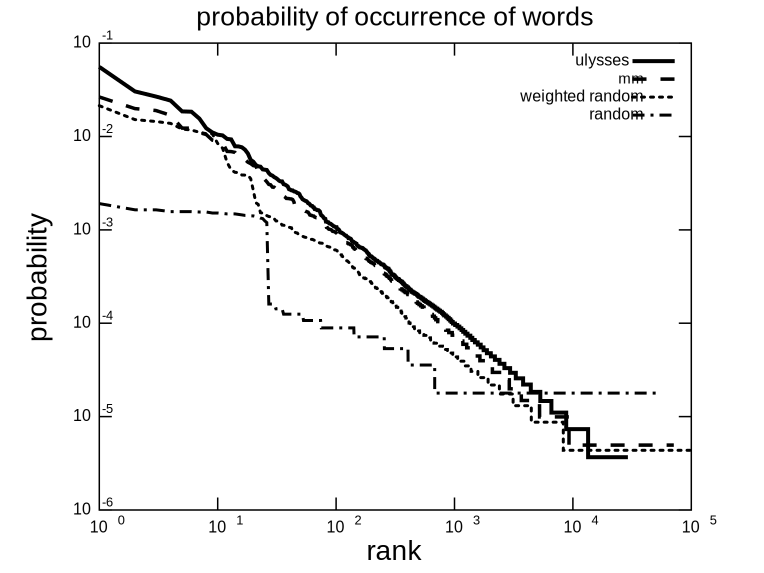
\includegraphics[width=0.8\textwidth]{images/ulysses_compared_words_probabilities.pdf}  
\caption{The rank-frequency distribution of (pseudo-)words in James Joyce's \textit{Ulysses} and random texts using the phones/diphones probabilities. The random curve presents the frequency of occurrence of pseudowords derived by text created by a white process and having the same length as \textit{Ulysses}. The weighted random curve is created by randomly choosing symbols with the same probabilities as the phones in \textit{Ulysses}. The \textit{mm} curve presents the result of a random text derived by a Markov Model where the transition between phones has the same probabilities of the transitions found in \textit{Ulysses}.}
\label{fig:ulysses_compared_words_probabilities}  
\end{figure}  
 
 
Zipf also presents the comparison curve of R. C. Eldridge data, which consists of 
43,989 running words, with 6,002 different words, of combined samples from American
newspapers. The concordance on the curves ``clearly show that the selection and usage
of words is a matter of fundamental regularity of some sort of an underlying governing
principle that is not inconsistent with our theoretical expectations of a vocabulary
balance as a result of the Forces of Unification and Diversification'' \cite{zipf1949}.


The Zipf curves, as presented in Figure \ref{fig:ulysses_compared_words_probabilities}, 
must inherently be a monotonically decreasing curves, since the data is ordered and ranked
according to the frequency of occurrence. \cite{li1992} points that 
``Zipf's law is not a deep law in natural language as
one might first have thought. It is very much related to the particular representation one
chooses, i.e., rank as the independent variable''. 
If Zipf's law arises at randomly generated texts with no linguistic structure, we might conclude
that the law may be a statistical artifact rather than a meaningful linguistic property.

Random generated sequences of letters results in the formation of letter chunks. Those letter chunks
might be sorted according to their frequency of occurrence and, by doing that, chunks of the same
length will present approximately the same frequency, what will create a stair case pattern as presented 
by \citet{li1992}. The decay follows approximately a Zipf's law slope
$(\sim 1/r)$, a power law with exponent $1$ (one). 
The results presented in Figure \ref{fig:ulysses_compared_words_probabilities} shows that
white random text follows clearly a different pattern compared to the natural text,
but as the random generator process assumes certain characteristics, it might have a pattern
closer to the one found in natural texts.

The simple model considered by \citet{li1992} is due to \cite{miller1957,mandelbrot1965}
and it is known as \textit{random typing} or \textit{intermittent silence} model.
It is simply a random generator of characters, where a certain symbol is designed as 
a word-delimiting character. As seen here, the words formed by this approach
show a Zipffian-like frequency behavior, but the number of different words of a certain
length is exponential in length, what diverges from what is observed in a natural language,
since it is in fact not even monotonic.
The \textit{intermittent silence} model might not be used to draw a conclusion that
the Zipf's law is linguistically shallow \citep{mandelbrot1982}, since that model is ``shallow'' itself.


Considering that the probability of occurrence of phones in a random generated text is not uniform,
we experience different results that distance from the white random case and get closer to the natural text.
Figure \ref{fig:ulysses_compared_words_probabilities} presents three different randomly generated texts:
1) equal probability phones, white noise (depicted by dashed-point line); 2) weighted probabilities, using 
the same probabilities of the phones encountered in \textit{Ulysses} (small dashed line); 3) text generated
by a Markov Chain using the states' transitions probabilities equal to the probabilities in \textit{Ulysses} 
(big dashed line).

In a natural language not all combinations of speech structures are possible, and they don't happen
with the same probability. We might observe this when comparing the number of existing words for a given
length. When a random generation process is used, the number of different words (types) will be greater  
then the number of words in a natural language, and that will be valid for every word length.
What we observe is that a natural language presents a higher probability of occurrence for small
words. In our compared example, the highest probability occurs on words of length $4$ and $3$.
This behavior is quite different from the random patter, as we might observe in Figure
\ref{fig:ulysses_compared_word_length_probabilities}.


\begin{figure}[h]
\centering  
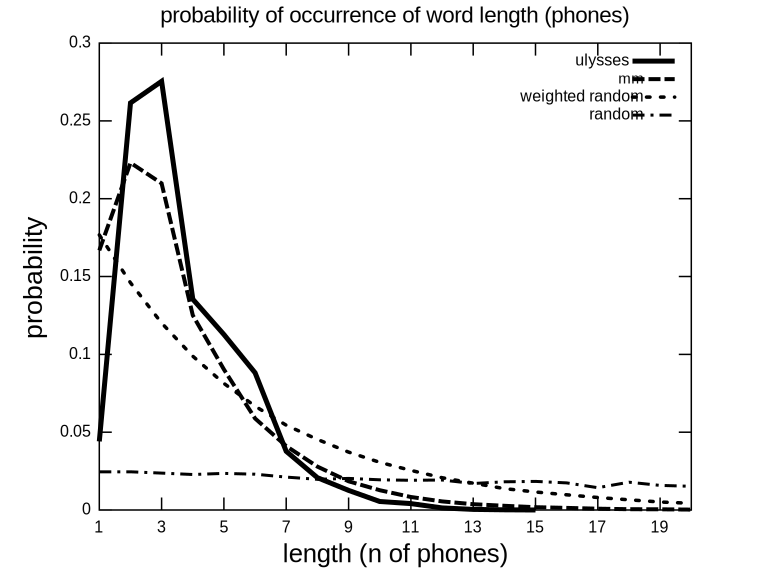
\includegraphics[width=0.8\textwidth]{images/ulysses_compared_word_length_probabilities.pdf}  
\caption{Compared plot of the frequency of occurrence of (pseudo-)words length in \textit{Ulysses} and random texts as described in the text.}
\label{fig:ulysses_compared_word_length_probabilities}  
\end{figure} 

It is important to note that when we consider the random generated texts, we are generating a
string of symbols that we are regarding as phones, and for that reason we consider a set with
the same size of the set of phones. This assumption is made because we are assuming that phones
are our unity of analysis. When we are dealing with natural text, we are using a phonetic
transcription dictionary, as previously stated.

The examples of random generated text in Figure \ref{fig:ulysses_compared_word_length_probabilities}
show that when we consider a weighted probability of occurrence for the randomly generated symbols,
we create the effect of making the shorted pseudo-words more probable, but what we observe in a
natural language is different, we don't see a monotonically decreasing probability, but rather
a peak on words of length $4$. This effect is slightly achieved when we consider a Markov Model with
transitions probabilities equals to the probabilities found in the natural text.
To explain the behavior observed in Figure \ref{fig:ulysses_compared_word_length_probabilities}, we 
might consider the role of three forces: 1) a human cognition ability that makes us assign
shorted codes to more frequent signs, this effect causes a tendency in the probability to 
monotonically decay as the length of words increases; 2) the number of possible symbols chunks that
might be created, regarding that the symbols probabilities are not uniform, this will also 
creates a monotonically decreasing probability patter; 3) there are restrictions imposed on
certain combinations of phones, provoking a greater effect on short words, due to the smaller
amount of possible combinations of symbols. We could also hypothesize that there are restrictions
on the sequence of phones that overcome the immediate vicinity of that phone, and this effect 
would be stronger on phones that are closer, and weaker on phones that are far apart, 
also causesing the smaller probabilities on very
short chunks, where this restriction poses a stronger force, and being overcome on longer ones.







\subsection{The Analysis of Smaller Units}
\label{sec:smaller_units}
In the previous analysis we focused on words as our speech units.
Word is considered the smallest free form that can be uttered or written and carries a meaning.
This is the concept introduced by \citet{bloomfield1926}, but it is doubtful, since some words are not
minimal free forms, like \textit{the} and \textit{of}, which carry no meaning by themselves.
The status of words in a language is still a topic over debate and with not clear answers.
``Words are units at the boundary between morphology and syntax serving important functions as carriers of both semantic and syntactic information and as such are subject to typological variation. In some languages words seem to be more clearly delimited and more stable than in others. The structural make-up of words depends on typological characteristics of languages'' \citep{coulmas}.


The main concern in Phonology is the study of language, as a means of spoken communication, that is built as a system
created by sounds and structures. Under the phonological assumption, 
the concept of sound is not restricted at the physical level of speech
realization, but also extends to symbolic level, where \textit{sounds} are cognitive abstractions
that provide the means for the representation of a language.

The Swiss linguist Ferdinand de Saussure is responsible for
shifting the way linguistic was done and established a break point with his posthumous
publication \textit{Course in General Linguistics} in 1916.
Although many years have passed, the central concept of relating sound to meaning in a structured way 
has remained the same. In Saussure's model, the linguistic sign has three aspects: 
physical (sound waves), physiological (audition and phonation) and psychological (sounds as abstract units,
which he calls `sound images').

The concept of \textit{sound images} was represented by the phoneme, regarded as a linguistic distinctive unity
which groups different sounds into single and not superposed categories.
Each language has its own phoneme inventory, which is created by what are the possible distinctions made between 
speech sounds in each language. For example, English makes no distinction between aspirated and unaspirated sounds,
but in Hindi such distinction exists \citep{ladefoged1996}.
Implicit in the idea of phoneme is that language may be segmented into a sequence of
consecutive symbols in time. %Beno\^it Mandelbrot 
\citet{mandelbrot} showed it is an important requirement
in order to make speech a comprehensible communication process in most situations,
especially under heavy corruption. This discrete aspect of language guarantees the discreteness at all other levels
of the language analysis, what is the basis of our linguistic knowledge.


As pointed out by \citet{capek1983}: ``Saussure did not discover -- or invent -- the phoneme.
He was one of a number of scholars working on comparable ideas. His statements are
important not so much for the accuracy with which they report facts or for their strength
and consistency as for the explanatory power of the inferential network they set up. Suffice
it to say that after Saussure the clumsy terminology used by scholars who preceded him --
that of speech sounds (Sprachlaute) -- came to be replaced by the much more intuitively
satisfactory concept of the phoneme.''


The term \textit{phoneme} was proposed by the linguist Dufriche-Desgenettes
as a substitute for the German \textit{Sprachlaut} (\textit{speech sound}) in the early 1870s \citep{dresher2011}.
It had, by that time, the meaning of what we now call \textit{speech sound} or \textit{phone}.
The concept of \textit{phoneme} changed with Saussure, who used it ``to refer to a hypothesized sound in a 
proto-language together with its reflexes in the daughter languages'' and further the meaning was 
recast by Kruszewski, bringing the synchronic notion, that we have today, of a set of alternating elements 
that were interpreted by Baudouin as an invariant psychophonetic element that may be realized in different forms
and as proposed by Jones, a family of sounds that, for practical purposes, are
accounted as the same \citep{dresher2011}. Today the phoneme no longer holds a central place
in phonology theory, but it has not disappeared from phonological theory nor its demise has come.
Although many evidences have risen questioning the phoneme status \citep{port2007,port2005,port2006}, 
its definition and properties, it seems more as a symptom of a theory of phonology that is not 
completely defined yet.


``The point of concern at present, however, is not to
devise a system of symbols whereby the sequence of sub-gestures constituting a speech-sound 
can be noted, but rather to remark that speech-sounds and phonemes may be
viewed as constellations, or configurations, of articulatory sub-gestures, arranged partly
or completely in sequential order, some sequences running concurrently with others (e.g.
the occlusion is concurrent with the voicing of \textit{d}). Although there is not a single speech-sound, 
or variant form, of a phoneme in any language which cannot be conceived of as a
constellation or configuration of the type envisaged above, yet a complete and accurate
description of even a single speech-sound in terms of sequences is practically impossible.
However, by conceiving phonemes as constellations of this order, we have found a very
useful method of comparing a number of specific phoneme pairs which have essential
sequences in common''\citep{zipf1949}.


The units of language (phonemes, syllables and words) are well represented in a writing system,
for the process of writing requires the dissection of the
speech stream into its constituents distinguishable parts. The process of dissection happens in
different levels, so that the assemblage of its parts creates meaning on the speaker discourse.
``Every writing system maps onto a linguistic system, it embodies and visibly exhibits the 
dissection of units of language and thus linguistic analysis''\citep{coulmas}.
It is reasonable then to investigate the patterns and structures of a language through its
written counterpart.


In order to perform such analysis, we used the text \textit{Ulysses} from
Joyce, and created a transcription from written text to phones sequence. 
The Carnegie Mellon University (CMU) 
Pronouncing Dictionary \citep{cmu2008} was used to get the phonetic transcription of each word in our database,
according to the General American (GA) English, which is
the major accent of American English. 
In the CMU Pronouncing Dictionary, words are coded by the phonetic transcription code \textit{Arpabet},
where each code is a distinct sequence of ASCII characters.
GNU tools, Python and Octave scripts were used to process and analyze the data.


\subsection{Phones, Diphones and Triphones}
\label{sec:phones}
In this section we present the results observed as we draw a Zipf plot of the phones, diphones and
triphones, comparing the natural text with the random generated texts, as previously described.
Figure \ref{fig:ulysses_compared_phones_probabilities} presents the compared probability of occurrence
of phones. As all random texts were generated using the phone probabilities or
transition probabilities from \textit{Ulysses}, they presented the same behavior, only the
white random process shows a different result, since all phones are equiprobable.
There are 39 phones, and from a visual inspection of Figure \ref{fig:ulysses_compared_phones_probabilities}
we might conclude that the Zipf's law does not holds for this very small set of symbols,
%we could conclude that the first 28 phones follow a Zipf relation different from the other 11 phones.
%We observe that it does not follow a Zipfian
%distribution, 
but instead a logarithmic relation exist, as also pointed by \cite{kanter1995}.
As we analyze higher order structures, we shall notice that it will progressively approach 
a Zipf's relation as we go from phones to diphones, then from diphones to triphones, until
we reach the words' level, which clearly presents a Zipf's law.
%There is a clear change in behavior that is not found when we analyze higher level structures,
%such as diphones, triphones, and words.


\begin{figure}
\centering
\begin{tabular}{cc}
  \subfloat[Comparison of phone frequency of occurrence. All three curves present the same pattern.]{\label{fig:ulysses_compared_phones_probabilities}\includegraphics[width=0.45\textwidth]{images/ulysses_compared_phones_probabilities.pdf}} &
  \subfloat[Comparison of diphone frequencies of occurrence. The behaviour of diphone frequencies generated by the white and weighted random text diverges from the others.]{\label{fig:ulysses_compared_diphones_probabilities}\includegraphics[width=0.45\textwidth]{images/ulysses_compared_diphones_probabilities.pdf}} \\
  \subfloat[Comparison of triphone frequencies of occurrence. The behaviour of triphone frequencies generated by the Markov Model does not follow closely the pattern presented in \textit{Ulysses} as was still observed with diphones.]{\label{fig:ulysses_compared_triphones_probabilities}\includegraphics[width=0.45\textwidth]{images/ulysses_compared_triphones_probabilities.pdf}} &
  \subfloat[Frequency of occurrence of syllables in \textit{Ulysses}. The syllabification was done computationally using online dictionaries.]{\label{fig:ulysses_syllables_probabilities}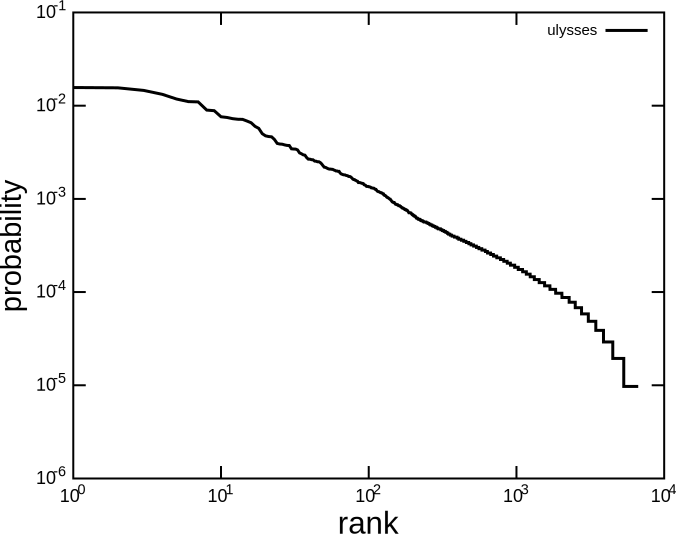
\includegraphics[width=0.45\textwidth]{images/ulysses_syllables_probabilities.pdf}}    
\end{tabular}
\caption{Compared frequency of occurrence plot for phones, diphones and triphones in \textit{Ulysses} and in random texts generated as previously described, a white random source; a weighted random source with phones probabilities equal to the one found in \textit{Ulysses}; and a Markov model with transition probabilities between phones as the probabilities in \textit{Ulysses}.}
\label{fig:ulysses_compared_nphones_probabilities}
\end{figure}


It is interesting to observe how phones occur in a language and the way they relate with one another
creating higher order structures under different constraints. The acquisition of a language is 
based on tracking those multiple regularities in the input stimuli. Only if we analyze long data
it will be possible to observe emergent regularities, and the more complex the regularities under
observation are, the more data will be needed to stablish a distinction among those regular patterns.
Those regularities are known as grammatical structure of a language, and since early ages, 
infants can perceive the difference of grammatical and ungrammatical sentences \citep{Saffran2003}.


The plot in Figure \ref{fig:ulysses_compared_diphones_probabilities} 
shows the probability of occurrence of diphones found in the same texts described before.
The white random process still preserves the equiprobability on the occurrence of diphones.
The Markov Model still follows very closely our reference text, and our zero order model 
does not present the same characteristic as the reference. 
When we take into consideration transition probabilities as our source model, 
we observe that the formation of some diphones is facilitated, while the formation of others 
is hardened. The behavior of phones clearly doesn't agree with a power law relation, but
not, observing the behavior of diphones we start to see a Zipf's law being created, as a result
of the increase on the length of our symbol set.
%The behavior of phones could be thought as two different Zipf laws, now the behavior of
%diphones might be interpreted as two Zipf laws with a smooth transition between them. 

As we move forward from phones, diphones and triphones to larger chunks, 
what we may observe is that the behavior gets closer to
the Zipf law observed when we analyzed words as our structural blocks. 
%It is still not 
%possible to state a single law to describe the observed data, but it grows near the word behavior
%in a Zipf plot. 
Observing the compared plot stated in Figure \ref{fig:ulysses_compared_triphones_probabilities}
we might observe that only the Markov model follows closely the natural behavior of triphones.
The frequency of occurrence, or predictability, of a speech unit is believed to be related to
its complexity when regarding acoustic realization \citep{jurafsky2001}, and the complexity is 
further associated with the duration of the given structure. Using annotated speech corpora,
\citet{jurafsky2001} concluded that when regarding the frequency of occurrence of n-phones as a function of its
duration, the relation is an inverted U-shape curve, so that short n-phones have smaller 
probability of occurring than middle-length n-phones and longer n-phones also have smaller 
probability. Comparing the frequency of occurrence of words for a given length we 
observed different results as we regarded phones or syllables as our building units for the words.
As previously shown in Figure \ref{fig:ulysses_compared_word_length_probabilities},
short words have smaller probabilities than middle length words, and the peak occurred in 3 phone
long words. When the length of a word is regarded as the number of syllables, then we
observed a monotonically decaying curve of probability of occurrence of words versus 
word length. Although there is not a clear straight relation between the number of syllables in a word
and its duration, from our observations in Section \ref{sec:words_length}, 
it seems reasonable to infer that the duration is proportional,
and that would lead again to the conclusion that, on higher order analysis, the 
behavior observed in the frequency of occurrence of words is different from its constituent parts.
The U-shape curve is reshaped into a straight line as syllables or phones are combined to build up
words.

It seems fascinating that languages and other natural phenomena, all of them a result of 
different complex systems, share a certain property which is described by a single simple law.
The same patterns are also observed when analyzing words and n-phones in different languages.
\cite{miller1965} proposes two different approaches to explain the ubiquitous observation of
Zipf's law: ``Faced with this massive statistical regularity, you have two alternatives.
Either you can assume that it reflects some universal property of human
mind, or you can assume that it reflects some necessary consequence of
the laws of probabilities. Zipf chose the synthetic hypothesis and searched
for a principle of least effort that would explain the apparent equilibrium
between uniformity and diversity in our use of words. Most others who
were subsequently attracted to the problems chose the analytic hypothesis
and searched for a probabilistic explanation. Now, thirty years later, it
seems clear that the others were right. Zipf's curves are merely one way
to express a necessary consequence of regarding a message source as a
stochastic process''.

Larger units of speech are used as recognition units to model the coarticulatory effects,
for example, syllables and triphones. The last one is quite often used in phonemic based
speech recognition, for the context of a given phone is established by its preceding and
following neighbors. 
The more features subsequent phonemes share, more easier will be the articulation of this 
sequence, since the transitions tend to be smother. On the other hand, it is important 
to create contrast between adjacent phonemes, so that one phone is distinguishable
enough from the phone next to it, what will enhance discriminability. This tradeoff
might be perceived on the triphones usage profile. 
Figure \ref{fig:ulysses_triphones_intradistances_mesh} presents the probability of occurrence of
triphones given their intradistances. For each triphone, two distances are calculated: the
distance from the second to the first phone; and the distance from the last to the middle phone.
The distance measure used is the number of distinctive features not shared by two phones under comparison,
as is explained in Chapter \ref{cp:featuretheory}. The number of occurrences of each triphone occurring in 
\textit{Ulysses} was added up 
according to its intradistances and the final probability of occurrence for each intradistance pair 
was calculated. We might observe in Figure \ref{fig:ulysses_triphones_intradistances_mesh}
that the most occurring triphones are those with medium intradistances, which appear as
a peak. That makes evident the tradeoff, previously argued, between articulatory ease and contrast.  
Triphones with small and large intradistances are seldom used, and some intradistance pairs
(26 in the total, which represent 11.5\% of the 225 possibilities) are not used at all.


\begin{figure}[h]
\centering  
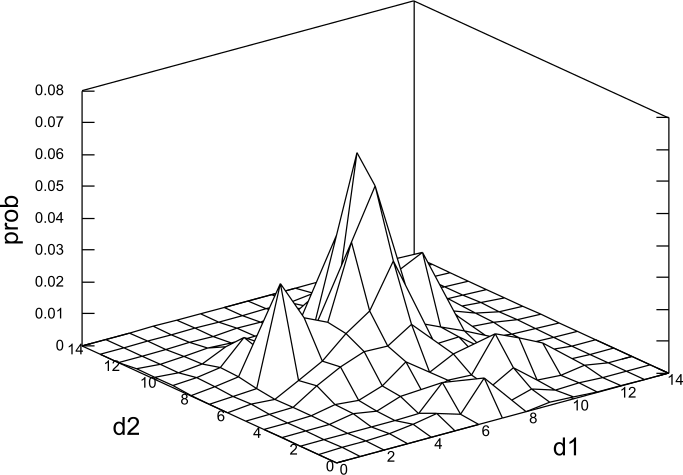
\includegraphics[width=0.8\textwidth]{images/ulysses_triphones_intradistances_mesh.pdf}  
\caption{Given the intradistances in a triphone (the distance from the second to the first phone, $d_1$, and the distance from the third to the second phone, $d_2$), the probability of occurring triphones in \textit{Ulysses} is presented. Triphones privileges medium intradistances, having a peak when the intradistances are around 8. The distance function used the number of non-shared distinctive features.}
\label{fig:ulysses_triphones_intradistances_mesh}  
\end{figure} 


Figure \ref{fig:ulysses_triphones_intradistances_mesh} shows that there is a strong relationship 
between adjacent phones in a triphone structure, where the inter-distance between phones tend to
an average value, and extreme values are not usual. It is natural then to speculate what would be
this kind of relation within words. Figure \ref{fig:ulysses_words_intra_phone_distance_freq_occ_avg_std}
provides an analysis of the inter-phone distances within words. It presents, in a logarithmic scale,
the frequency of occurrence of words for a given relation between the average inter-phone distances and 
the standard deviation of the inter-phone distances. Once again, the distance metric used is the number
of distinctive features not shared by two phones. Among the plotted data, we observe no tendency of increased
occurrence of words for a certain relation between average and standard deviation of inter-phone distances.
The plot of the number of words for a certain relationship of their inter-phone distances present a similar
pattern, and normalizing the frequency of occurrence chart by chart with the number of words, we
conclude that there is no aid making some inter-phone distance relation more probable than others.
What we might observe from our chart and analysis is that there is a relationship between the
average value and the standard deviation value for the inter-phone distances: when the average distance
decreases, the deviation increases as a compensatory effect, for words have to maintain a certain phonemic 
variability within. The correlation coefficients (Pearson product-moment correlation coefficient)
between the mean value and the standard deviation observed in the inter-phone distances within words
is $-0.67$ and p-values for testing the hypothesis of no correlation
(assuming that the true correlation is zero, the p-value is the probability of getting a correlation as large 
as the observed one)
is null.


\begin{figure}[h]
\centering  
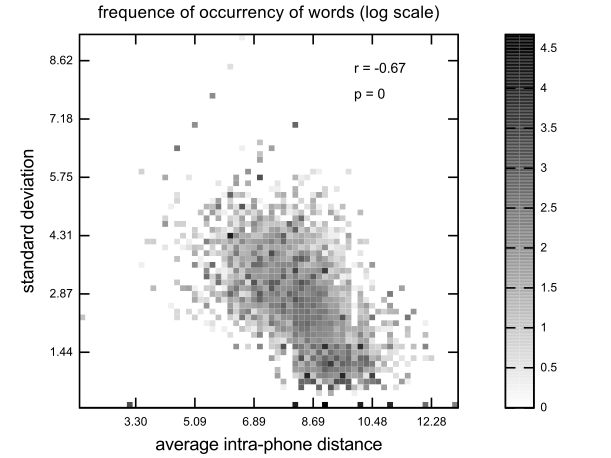
\includegraphics[width=0.8\textwidth]{images/ulysses_words_intra_phone_distance_freq_occ_avg_std.pdf}  
\caption{The words frequency of occurrence  in \textit{Ulysses} is presented in a logarithmic scale as a function
of the average intra-phone distances and the standard deviation of these distances. The relationship
between the number of existing words as a function of average and standard deviation of distances follows
a similar pattern and our analysis doesn't show any effect that frequency has on this pattern. 
What we might observe is the tradeoff between average intra-phone distance and standard deviation, 
as the mean distance value decreases, the deviation increases as a compensatory effect. 
The correlation coefficient observed in this data (with 19,150 samples) is $-0.67$.}
\label{fig:ulysses_words_intra_phone_distance_freq_occ_avg_std}  
\end{figure} 


In order to analyze the variability of triphones that may be formed by a certain phone, 
when regarding the transitions of distinctive features in a triphone, we 
considered the difference of the distinctive feature vectors between the middle phone
(reference) and the first and last phones. As each reference phone occurs in many
triphones combinations, we create a weighted sum of all these difference feature vectors, 
where the weight factor is the probability of occurrence of each triphone. For each
phone we have built two vectors: one from the differences with the previous phone
and the other from the differences with the next phone.
Each of these vectors is represented by a column in the image presented
in Figure \ref{fig:phone_triphone_varialibity_dist_features_sorted2}.
It is presented as shades of gray, when the gray level approaches white,
then there is more variability (the difference is greater) and when it approaches
black, there is less variability (the difference is smaller).
We have ordered the features sorted by the accumulated variability across 
all different triphones for all phones in the set. The cumulative curve is plotted on the right. 
We also ordered the phones
by the variability observed on their triphones. Each pair of columns 
in the image presented in Figure \ref{fig:phone_triphone_varialibity_dist_features_sorted2}
corresponds to one phone that is transcribed in the axis bellow.
The bottom curve in Figure \ref{fig:phone_triphone_varialibity_dist_features_sorted2}
presents the variability for each phone, 
displaying
the differences with the previous phone (left) and the differences with
the next phone (right) in a triphone set.
We might conclude that the features presented are sorted by their distinctiveness 
capabilities, that is: \textit{syllabic}, \textit{consonantal}, \textit{sonorant}, \textit{coronal}, 
\textit{back}, \textit{front}, \textit{continuant acoustic}, \textit{voice}, \textit{high}, 
\textit{strident}, \textit{labial}, \textit{approximant}, \textit{nasal}, \textit{distributed},
\textit{dorsal}, \textit{tense}, \textit{lateral}, \textit{labiodental}, \textit{delayed release}, 
\textit{spread glottis}, \textit{trill}, \textit{tap} and \textit{constricted glottis}.


From the bottom plot in Figure \ref{fig:phone_triphone_varialibity_dist_features_sorted2}
we might conclude that the variability between the first and the middle phones in a triphone
is always greater than the variability between the middle and the last phones.
Since every two side-by-side points corresponds to one certain phone, and they are always arranged 
in the order mentioned before (1st-2nd phones, 2nd-3rd phones), 
we observe that within each pair the curve presents a negative slope,
and for that reason we might conclude that the first phone pair (1st-2nd phones) has a greater distinctive
feature variability in every triphone.
As we analyze larger chunks, we verify that this decreasing behavior on the average distance
between phones does not hold anymore.

\begin{sidewaysfigure}
%\vspace{12cm}
\centering  
\includegraphics[width=0.8\textwidth]{images/phone_triphone_varialibity_dist_features_sorted2.pdf}  
\caption{This picture presents the variability of distinctive features within triphones for a given
middle phone taken as reference. The distinctive features are sorted by their total variability 
(across all triphones) and the reference phones are sorted by the total variability across of its 
features within its set of triphones. The shades of gray represent the variability of a given 
feature within a give triphone. The white color correspond to the greatest variability and the
black color to the smallest variability.}
\label{fig:phone_triphone_varialibity_dist_features_sorted2}  
\end{sidewaysfigure}




Preliminary studies show the existence of consistent frequency distribution patterns in other languages.
These regularities are believed to be a result of language as a stochastic process and a product
of usage and self-organization. If the underlying principle of organization of languages is the same,
we are supposed to observe similar patterns when analyzing language statistics.







\section{Length of Words}
\label{sec:words_length}
The study of language, under a phonological point of view, presupposes
the discretization of the speech stream into unities, which are subject to rules.
Phonological theories are based on the discretization of speech into segments
that assembles themselves according to certain rules to create higher order
structures. 
Words are assumed as discrete entities built over other discrete
units, such as syllables, morphemes and phonemes.

Words are argued to be unities of mental representation,
although the very concept of word is still, in some aspects, unclear.
\cite{bloomfield1926} introduced the concept of words as the 
smallest free form that may be uttered in isolation carrying a semantic 
or pragmatic content of its own, but it is doubtful since some words are not minimal free forms.
It is fair to question whether or not
the definite and indefinite articles, \textit{the} and \textit{a}, are themselves words at all.
Do they carry a meaning of their own? 
There are also those meanings that require two strings of letters to express themselves, like: 
\textit{stock market}, \textit{apple tree}, \textit{carbon dioxide}, \textit{dental floss}, among others. 
What about \textit{compound words}? Is every \textit{compound word}
a word? Or a composition of words as the name suggest? 
There are many examples of \textit{compound words}: \textit{newspaper}, \textit{thumbnail},
\textit{copperhead}, \textit{eyelid}, \textit{bedroom}, among many others;
and there is also a tendency of some to become a \textit{compound word}, for example:
\textit{hot dog} it also written as \textit{hotdog}.
The compound word \textit{blackboard}
is just a combination of the words \textit{black} and \textit{board} that happens to designate
an object that is not black at all. What amount the uncountable examples that an analytical language
as German is capable of creating? The word for \textit{blackboard} in German is \textit{Tafel}, but
it could also be \textit{Wandtafel}, which is just a compound made of \textit{Tafel} and \textit{Wand}
(Wall). The German word \textit{Streichholzschachtel} (matchbook), is made of
\textit{streichen} (scratch), \textit{Holz} (wood), \textit{Schachtel} (box), while the English
word \textit{matchbox} is also a compound but made of \textit{match} (not the Football one) and
\textit{box}. The way they are built is quite different, but make reference to the same object.
That is something that tells about the way languages are structured and used, and it might be
possible that the structures are a bit different in every language. 

\cite{olson1994} stresses the point
that the concept of the word as distinct unit is a by-product of literacy acquisition.
The analysis of antique texts revels that texts were commonly redacted in \textit{scriptura continua},
that means `without word boundaries' \citep{saenger}. The continuous string of characters 
was just a rightful representation of what speech utterances truly are.
According to \citep{saenger1997}, the lack of boundaries between words causes 
two drawbacks in the reading process: it slows down reading and encourages vocal activity.
If the writing is dense and devoid of `distinguishing signs', the decoding process
is considerable longer and rely on vocalization. Silent and rapid reading is an achievement 
of our civilization which resulted from the development of a system of graphic signs in which
the blank space is of prime importance. ``In the sixth century, all manuscripts were still copied
in \textit{scriptura continua}, and it was not until between the sixth and eighth centuries that the
separation of words was progressively introduced into all Latin manuscripts'' \citep{pombo2002}. 
Literacy is indeed an influential ability in our languages skills. As pointed by \cite{hagege1986}
``writing is a linguistic analysis in various degrees of awareness''.

There are many interactions between speech and writing. Lev S. Vygotsky was a
psychologists who took an active interest in the cognitive consequences of writing,
studying how speech affected writing and vice versa. 
``Writing requires deliberate analytic action on the part of the speaker\footnote{Originally Lev S. Vygotsky was talking about \textit{child}, but we made the substitution to comprise a wider context which
we believe is still valid.}.
In speaking, he is hardly conscious of the sounds he produces and quite unconscious of
the mental operations he performs. In writing, he must take cognizance of the
sound structure of each word, dissect it, and reproduce it in alphabetic symbols,
which he must have studied and memorized before''\citep{vygotsky}.
The relationship between writing systems and spoken language is also a theme covered
by \cite{coulmas}. According to him, ``the introduction of writing implies a 
cognitive reorientation and a restructuring of symbolic behaviour. Names of objects
are conceptually dissociated from their denotata, as signs of physical objects are
reinterpreted as signs of linguistic objects, names. In a second step, signs of names
are recognized as potentially meaningless signs of bits of sound, which are then
broken down into smaller components'' \citep{coulmas}.

Considering words as unities of mental processing, it is important to investigate
the aspects involving this hypothesis. \cite{miller1956} suggested that the short-term memory
storage capacity is constant in terms of the number of chunks. If we could consider words as
chunks, then the short-term memory capacity should be the same regarding the size or duration
of words.
\cite{Baddeley1975} explores the relations between the memory span\footnote{Memory span is a common
measure for short-term memory, where it is related to the length of a list of discrete items a person 
is capable of memorize and repeat back in order after presentation with an accuracy equals of superior
to 50\% of all trials. It appears to measure one's capacity to successfully distribute his attention
and organize the incoming stimuli as a working unit.
} and length of words.
They observed that memory span is inversely proportional to word's length. Word's duration
was recognized as an important aspect, since it was recognized that words of short temporal duration were 
better recalled than words of long duration, even when the number of syllables and phonemes 
are held constant. 
The results achieved by \cite{Baddeley1975} have some implications on \cite{miller1956}'s 
suggestions, ``that memory span is limited in terms of number of chunks of information, rather that their
duration. It suggests a limit to the generality of the phenomenon which Miller discusses,
but does not, of course, completely negate it. The question remains as to how much
of the data subsumed under Miller's original generalization can be accounted for in terms
of temporal rather than structural limitations''\citep{Baddeley1975}.

\cite{neath1995} points that ``current explanations of the word-length effect
rely on a time-based decay process within the articulatory loop structure in working memory'',
what does not completely explain one of the observations made by \citep{Baddeley1975}: ``when
articulation is suppressed by requiring the subject to articulate an irrelevant sound, the
word length effect disappears with visual presentation, but remains when presentation is
auditory''. \cite{neath1995} concludes that ``word-length effects do not offer sufficient
justification for including time-based decay components in theories of memory''. He proposes
then a feature model \citep{nairne1988, nairne1990} where the interferences handles 
the explanation of the observed data.
It was designed to account for the major effects observed in immediate memory settings,
what includes the recency effect, the effects of articulatory suppression, temporal grouping, and
phonological similarity, among others. 

In order to better understand the role played by these aspects into the way a language is
structured, organized and used, we propose here a statistical analysis using a corpus. 
It would be time-spending and would require a great amount of work to collect a speech corpus
and make use of it. Instead, we propose the usage of a text corpus, pronunciation dictionary
and speech samples provided by online dictionaries.
The analysis here will concern only the statistical aspects of written and spoken words length,
what is important as length is regarded as an aspect of mental representation, 
among other features \citep{port2007}.

Mendenhall realized that the study of word length, specifically, the analysis of the distribution
of words of different lengths was important to establish comparisons of styles. \cite{mendenhall1887}
investigated the differences in the literary 
styles of Dickens and Thackeray insofar as word-length distribution was concerned. The same approach
was afterwards used \citep{mendenhall1901} to analyze the authorship of Shakespeare's plays\footnote{
The Shakespeare authorship question was first posed in the middle of the 19th century,
when the flattery of Shakespeare as the greatest writer of all time had become widespread.
More than 70 authorship candidates have been proposed, including Francis Bacon.}.
In every Shakespeare's play the count of words of length four was always greater than the count of
words of length three. Comparing with Bacon, the count of words of length three was greater than four, and
Bacon also present a distinctly higher proportion of longer words than Shakespeare.

Mandelbrot \citep{mandelbrot} supposes that words are built of a sequence of elementary unities and the process of 
assembling those unities into a speech stream is an elementary additive process. The cost
assigned to this process is a compound of the number of building blocks used and their characteristics.
The probability of occurrence 
of each word is assigned so that, on a long sequence, the average word-information-content
is maximized, being also subject to the additive costs of building each unity and the sum of
all the relative frequency of occurrence (probabilities) of each word must be one. Making the choice
that leads to such maximization is performing an entropy\footnote{As defined by Shannon, 
the entropy is an additive measure of the amount of available choice 
in the process of selecting one from the allowable messages among many in each unit of
the information transmission process. Entropy is used as a measure of the amount of information
carried by a random variable.} maximization.
The sender should maximize the transmission rate of information and concomitantly minimize
the cost of transmission. This cost was expressed as a function of the length required in the transmission
process, making short words a preferred choice. Mandelbrot demonstrated that a word-by-word encoding
of a message will lead to the observed rank-frequency relation in natural languages.

Using our database we are able to estimate the number of words for a given length and
also how frequently words of this length are used. The Figure \ref{fig:wordsNumVsLength} presents
these results. When the length of a word increases, the number of possible combinations of
building unities increases factorially, but what we observe is an increase as short length words
become longer and a great decrease after a turning point. The usage of shorter words, as expected,
is greater, and the small drop observed for small words is just a consequence of the fewer 
number of possible combination leading to the existing words with short length words. 
When the frequency of occurrence curve is normalized
by the the number of existing words, we get a monotonically decreasing line, as expected 
(Figure \ref{fig:wordslengthfreqnorm_en} and \ref{fig:wordsphoneslengthfreqnorm_en}). 
This is corroborated when we take the average word length across
words rank, as pictured in Figure \ref{fig:averagewordslength_en} and \ref{fig:averagewordsphoneslength_en}
the words with smaller rank are on average also smaller, either in the number of letters, phones
or syllables.

Figures \ref{fig:wordsFreqOccurrenceRange} and \ref{fig:phonesFreqOccurrenceRange}
present how the usage of words and phones is different when analyzing words of different
length (number of letters, number of phones or number of syllables).
It is possible to verify that in the extreme cases, when we analyze words of short length or 
long length, the pattern observed in the rank vs. frequency plot is quite different from the
middle length words. The short and long words experience steeper decay regarding the occurrence
of words or phones.


The relationship between the number of Phones and the number of Letters and 
the number of Phones and the number Syllables may be observed in 
Figure \ref{fig:wordsLettersPhonesSyllablesNumberOfWordsLog}.
Phones and Letters have a straight line relationship, and the majority of the words
have between 3 and 9 letters and 3 and 10 phones.
The relationship between number of phones and syllables is a little more dispersed,
and we may observe that the majority of words have between 1 and 3 syllables, corresponding
to the range of 3 to 9 phones. 

When considering the frequency of usage of words with a certain number of syllables and phones,
or phones and letters, we observe a more diffuse relation that still resembles the relations
regarding the number of words. This might be observed in 
Figure \ref{fig:wordsLettersPhonesSyllablesFreqOccurrenceLog}.

Another way to regard words length is to measure its duration when uttered.
Although each speaker will utter the same word with a different duration at each
trial, on the average, and under normal conditions, we expect to observe the same
duration, what might not differ much from one speaker to another, unless 
one suffer from some sort of aphasia, compromising the speaker elocution capabilities,
or he is under a certain situation in which he is required to speak on a much slower or 
faster rate. The data then here analyzed consists of utterance duration of words
collected from online dictionaries. The samples where collected from each dictionary and
its duration were afterwards normalized within each group. Unfortunately each dictionary has
samples from different speakers and there is no control under the speech rate used.
Although the data don't present
a strong correlation it is not so weak and we might observe, in Figure \ref{fig:dicutterduration},
that the relation between number of syllable and duration of the uttered word is
more diffuse then the previous relations presented before, but still there is a 
straight line tendency.


\begin{sidewaysfigure}
  \centering
  \subfloat[number of letters.]{\label{fig:wordsNumVsLetterLength}\includegraphics[width=0.3\textwidth]{images/wordsNumVsLetterLength.pdf}}                
  \subfloat[number of phones]{\label{fig:wordsNumVsPhoneLength}\includegraphics[width=0.3\textwidth]{images/wordsNumVsPhoneLength.pdf}}    
  \subfloat[number of syllables]{\label{fig:wordsNumVsSyllableLength}\includegraphics[width=0.3\textwidth]{images/wordsNumVsSyllableLength.pdf}}    
  \caption{Number of words in the English with a certain length, measured as the number of letters, phones or syllables.}
  \label{fig:wordsNumVsLength}

  \centering
  \subfloat[number of letters.]{\label{fig:wordsFreqOccurrenceVsLetterLength}\includegraphics[width=0.3\textwidth]{images/wordsFreqOccurrenceVsLetterLength.pdf}}                
  \subfloat[number of phones]{\label{fig:wordsFreqOccurrenceVsPhonesLength}\includegraphics[width=0.3\textwidth]{images/wordsFreqOccurrenceVsPhonesLength.pdf}}    
  \subfloat[number of syllables]{\label{fig:wordsFreqOccurrenceVsSyllableLength}\includegraphics[width=0.3\textwidth]{images/wordsFreqOccurrenceVsSyllableLength.pdf}}    
  \caption{Frequency of occurrence of words in the English with a certain length, measured as the number of letters, phones or syllables.}
  \label{fig:wordsFreqVsLength}
\end{sidewaysfigure}


\begin{sidewaysfigure}
  \centering
  \subfloat[number of letters.]{\label{fig:wordsFreqOccurrence01-09Letters}\includegraphics[width=0.3\textwidth]{images/wordsFreqOccurrence01-09Letters.png}}                
  \subfloat[number of phones]{\label{fig:wordsFreqOccurrence01-09Phones}\includegraphics[width=0.3\textwidth]{images/wordsFreqOccurrence01-09Phones.png}}    
  \subfloat[number of syllables]{\label{fig:wordsFreqOccurrence01-07Syllables2}\includegraphics[width=0.3\textwidth]{images/wordsFreqOccurrence01-07Syllables2.png}}    
  \caption{Frequency of occurrence of words in English with length in a certain range, measured as the number of letters(\ref{fig:wordsFreqOccurrence01-09Letters}), phones(\ref{fig:wordsFreqOccurrence01-09Phones}) or syllables(\ref{fig:wordsFreqOccurrence01-07Syllables2}).}
  \label{fig:wordsFreqOccurrenceRange}


  \centering
  \subfloat[number of letters.]{\label{fig:phonesFreqOccurrence01-09Letters}\includegraphics[width=0.3\textwidth]{images/phonesFreqOccurrence01-09Letters.png}}                
  \subfloat[number of phones]{\label{fig:phonesFreqOccurrence01-09Phones}\includegraphics[width=0.3\textwidth]{images/phonesFreqOccurrence01-09Phones.png}}    
  \subfloat[number of syllables]{\label{fig:phonesFreqOccurrence01-07Syllables}\includegraphics[width=0.3\textwidth]{images/phonesFreqOccurrence01-07Syllables.png}}    
  \caption{Frequency of occurrence of phones in English within words with length in a certain range, measured as the number of letters(\ref{fig:phonesFreqOccurrence01-09Letters}), phones(\ref{fig:phonesFreqOccurrence01-09Phones}) or syllables(\ref{fig:phonesFreqOccurrence01-07Syllables}).}
  \label{fig:phonesFreqOccurrenceRange}
  
\end{sidewaysfigure}


\begin{sidewaysfigure}
  \centering
  \subfloat[Letters and Phones.]{\label{fig:wordsLettersPhonesNumberOfWordsLog}\includegraphics[width=0.3\textwidth]{images/wordsLettersPhonesNumberOfWordsLog.png}}                
  \subfloat[Phones and Syllables.]{\label{fig:wordsPhonesSyllablesNumberOfWordsLog}\includegraphics[width=0.3\textwidth]{images/wordsPhonesSyllablesNumberOfWordsLog.png}}      
  \caption{Number of English words with a certain number of letters, phones and syllables.}
  \label{fig:wordsLettersPhonesSyllablesNumberOfWordsLog}

  \centering
  \subfloat[Letters and Phones.]{\label{fig:wordsLettersPhonesFreqOccurrenceLog}\includegraphics[width=0.3\textwidth]{images/wordsLettersPhonesFreqOccurrenceLog.png}}                
  \subfloat[Phones and Syllables.]{\label{fig:wordsPhonesSyllablesFreqOccurrenceLog}\includegraphics[width=0.3\textwidth]{images/wordsPhonesSyllablesFreqOccurrenceLog.png}}      
  \caption{Frequency of occurrence of words in English with a certain number of letters, phones and syllables.}
  \label{fig:wordsLettersPhonesSyllablesFreqOccurrenceLog}

\end{sidewaysfigure}



\begin{sidewaysfigure}
  \centering
  \subfloat[Scatter plot of words utterance duration from four different dictionaries.]{\label{fig:corrWordsDurationDics}\includegraphics[width=0.3\textwidth]{images/corrWordsDurationDics.png}}                
  \subfloat[Histogram of words mean (across the four different dictionaries) utterance duration.]{\label{fig:histWordsMeanDuration}\includegraphics[width=0.3\textwidth]{images/histWordsMeanDuration.pdf}}
  \subfloat[Number of words with a certain number of syllables and a certain duration.]{\label{fig:numWordsSyllableVsMeanDuration_log}\includegraphics[width=0.3\textwidth]{images/numWordsSyllableVsMeanDuration_log.pdf}} 
  \caption{The data here presented uses the utterances duration of speech samples from the four following on-line dictionaries: Cambridge, Dictionary.com, The free dictionary and Macmillan. The durations were first normalized within each set from each dictionary. Only the words found in all the four dictionaries were used.}
  \label{fig:dicutterduration}
\end{sidewaysfigure}






%
%
%
\section{Menzerath's law}

\cite{menzerath1928} observed the relation between the average syllable length and 
the word length, regarding the number of syllables that build the word, was a
decreasing relationship, as the number of syllables in a word grew, the average length
of the syllables decreased. In general form, this observation would further be formulated as
a linguistic law according to which the increase of a linguistic construct results 
in a decrease of its constituents, and vice-versa. 
Examining the structures of German words, \cite{menzerath1954} stated the hypothesis:
``Je größer das Ganze, desto kleiner die Teile'' (the longer the whole, the smaller the parts).
This hypothesis did not apply solely to Linguistics, but we are here concerned with its implications
on the study of languages. That could imply that there is no uniformity in the units of
a language and the hypothesis could be specified as ``the complexer a linguistics' construct,
the simpler are its constituents''. This hypothesis seems plausible: linguistics's constructs
carry information and are made of specific constituents. The constituents are chosen
so that the construct may be clearly identified and they should have enough redundancy so that, 
even under severe interference, they might be distinctive one from another. For the reasons given,
short construct should be made of longer and more distinctive constituents, while for longer
construct shorter and less distinctive constituents might also be used, and the existence of redundancy
should be adequately secured to properly differentiate one construct from another.

In order to derive the relation between constructs and constituents, we may investigate the length
relationship between them. We may denote by $y$ the length of the constituent and by $x$ the length
of the construct. The change relative rate on the length of the constituent, the first derivative of
$y$ divided by $y$, is inversely proportional to the length of the construct. 
The increase of length of the constituent is also proportional to the length of constituent. 
Mathematically,
$y'/y \sim 1/x$, and we may then state in the following form:
\begin{equation}
\frac{y'}{y} = \frac{b}{x} \textmd{.}
\end{equation}
This differential equation my be solved directly by integration, resulting in
\begin{equation}
\ln y = b \ln x + c \textmd{,}
\end{equation}
From what follows that
\begin{equation}
y = a x^b
\label{eq:yaxb}
\end{equation}
where $a = e^c$, and therefore, this parameter is always greater than zero,
following then that the curve stated by Relation \ref{eq:yaxb} is a rising convex curve
when $b > 1$, it will be a concave rising curve when $0 < b < 1$ and it will be
a convex falling curve when $b < 0$.

\cite{altmann1980}
formulated mathematically the Menzerath's principle.
He considered also a disturbance, making the relation become
\begin{equation}
\frac{y'}{y} = \frac{b}{x} + c \textmd{,}
\label{eq:yybxc}
\end{equation} 
from which the solution is stated as:
\begin{equation}
y = a x^b  e^{c x} \textmd{ .}
\end{equation}
The curve will be monotonically decreasing when $-b/c > x$.
Considering the solution of Relation \ref{eq:yybxc}, we might argue whether
the perturbation arises or not from the parameters $b$ or $c$. Taking 
$b=0$, it will lead us to the third solution, which is
\begin{equation}
y = a e^{cx} \textmd{.}
\end{equation}

If the observed pattern does not agrees with the previous stated relations,
it doesn't necessarily implies a falsification of the Menzerath's law, but 
it could imply that other factors should also be taken into consideration,
for example, the position of a constituent in the construct \cite{altmann1989}.
Let us denote by $z$ the position of the constituent, meaning that it is
the $z$-th constituent inside a construct. The differential equation could 
then be rewritten as
\begin{equation}
\frac{y_x' + y_z'}{y} = - \frac{b}{z} + c \textmd{,}
\end{equation}
and the solution would be
\begin{equation}
y = az^b e^{cx} \textmd{.}
\end{equation}
The more factors are taken in account, the more complete and complex will get out
model.

%where $y$ stands for the constituent size (e.g. phone or syllable length),
%$x$ is the size of the linguistic construct (e.g. number of syllables or phones of a word),
%and the constants $a$, $b$ and $c$ are parameters of the relation. 


We present bellow, in Figure \ref{fig:boxplot_ulysses_words_avg_duration}, the relation
between construct (word) length (considering the number of syllables or phones it is made of), and
the average duration of its constituents (syllables or phones) or the average number of phones per syllables.
The Menzerath model was fitted using a least-mean squares procedure and the parameter obtained are 
presented bellow or in the Figure \ref{fig:boxplot_ulysses_words_avg_duration}, 
with the continuous fitted curve also displayed.

For the relation between words syllable length and average syllable duration the parameter found were:
$a = 743.166$, $b = -0.916$ and $c = 0.072$. For this model, the Pearson's correlation coefficient found
(between the data and the model's prediction) is $0.93$.
For the  relation between words phone length and the average duration 
of phones, the parameter were: $a = 619.87$, $b = -0.901$ and $c = 0.039$.
In this case, the correlation coefficient found was $0.91$.
For the last one, the relation between word syllable length and the average number of phones per syllable, the
parameter found were $a = 3.222$, $b = -0.451$ and $c = 0.067$. The correlation coefficient was $0.49$.
All models show the parameter $c$ close to zero, meaning that the simpler model, depicted
in Equation \ref{eq:yaxb}, would be suitable. For the last case scenario, the correlation between the model
and the data was poor, what leads that the model as proposed did not represent well the intrinsic relation,
and maybe some further considerations should taken, as previously discussed.

\begin{figure}
\centering
\begin{tabular}{cc}
  \subfloat[Average duration of syllables as the number of syllables in a word increases.]{\label{fig:boxplot_ulysses_words_avg_syllable_duration}\includegraphics[width=0.45\textwidth]{images/boxplot_ulysses_words_avg_syllable_duration_ms.pdf}} &
  \subfloat[Average duration of phones as the number of phones in a word increases.]{\label{fig:boxplot_ulysses_words_avg_phone_duration}\includegraphics[width=0.45\textwidth]{images/boxplot_ulysses_words_avg_phone_duration_ms.pdf}} \\
  \subfloat[Average number of phones per syllables as the number of syllables in words increases.]{\label{fig:boxplot_ulysses_words_avg_syllable_phone}\includegraphics[width=0.45\textwidth]{images/boxplot_ulysses_words_avg_syllable_phone.pdf}} 
\end{tabular}
\caption{The pronunciation duration of each word is the average of the speech sample from four different online dictionaries (Cambridge Dictionary, Dictionary Reference, The Free Dictionary and Macmillan Dictionary). The Boxplots display the relation between the words length (number of phones or number of syllables) and the average duration of its constituent parts (phones or syllables). The last Figure also presents the relation between the average number of phones per syllables as a function of the syllable length of words.}
\label{fig:boxplot_ulysses_words_avg_duration}
\end{figure}


%boxplot_ulysses_words_avg_phone_duration_ms_.pdf  boxplot_ulysses_words_avg_syllable_duration_ms_.pdf  %boxplot_ulysses_words_avg_syllable_phone.pdf
%boxplot_ulysses_words_avg_phone_duration.pdf      boxplot_ulysses_words_avg_syllable_duration.pdf


The Menzerath's relationship was previously presented in various levels of language units.
Going towards an upper level of syntactic generalization, we could expect to see that same relationship
on the word-sentence level. As depicted in Figure \ref{fig:ulysses_words_sentence_word_length},
it appears that an intermediate unit must be introduced between words and sentences \citep{kohler2005}.
This intermediate unit might be phrases or clauses, which are regarded as direct constituent of
sentences, as stated by \cite{grzybek2006}. Figure \ref{fig:ulysses_words_sentence_word_length} presents the
relation between words length (average number of characters that words are made of in a given sentence)
and sentence length (number of words in the given sentence). Each dot in this Figure represents 
a sentence in \textit{Ulysses}, by James Joyce. We might observe that, as sentences get longer,
the average word length tends to converge to the value of $4.46$. That could be reasoned as 
the result of two interacting forces, one tending to make words shorter as the sentences grow
longer, and another tending to make words longer. The equilibrium would be found in the
average word length of $4.46$. 

\cite{altmann1983}, interpreting the results related to the Menzerath-Altman Law, pointed out that
the relationship described by the law is more likely to hold true only if we are dealing with
direct constituents of a given construct.
From that observation and from the results observed in Figure \ref{fig:ulysses_words_sentence_word_length}, 
we might conclude that at least one intermediate
unit in the linguistic construct levels is necessary. \cite{buk2007} suggest the usage of clauses
and present results from the analysis of Ukrainian texts.
As a result, words may be considered as a direct constituent of clauses, but not of sentences.

The convergence of the average word length presented in Figure \ref{fig:ulysses_words_sentence_word_length}
might be a result of the low frequency presented in the analyzed text for long senteces,
as might be observed in the frequency vs. sentence length plot in Figure \ref{fig:ulysses_words_sentence_word_length_freq}.
It might also be that what drives this convergence a psycholinguistic motivation rather than an statistical one.
Regarding the human processing limits, as presented by \cite{miller1956}, there is a magical rule of
$7 \pm 2$, what could serve as a limitation on the average length of words in phrases or clauses.
 

% ulysses_words_sentence_word_length.png
\begin{figure}[h!]
\centering
\includegraphics[width=0.75\textwidth]{images/ulysses_words_sentence_word_length.png}
\caption{Average word length (number of letters) versus sentence length (number of words).
The mean word length average value is $4.46$.}
\label{fig:ulysses_words_sentence_word_length}
\end{figure} 


\begin{figure}[h!]
\centering
\includegraphics[width=0.75\textwidth]{images/ulysses_words_sentence_word_length_freq.pdf}
\caption{Frequency of occurrence of sentences for a given length.}
\label{fig:ulysses_words_sentence_word_length_freq}
\end{figure} 


Investigating the relation between sentences length and average words length, 
but this time, using the number of syllables as the unit to measure a word length,
we observe quite a different behavior, as it is presented in Figure \ref{fig:ulysses_words_sentence_word_length_syllables_z100}.
The analysis was again based on the text \textit{Ulysses}. Each word, in each sentence,
were transcribed into syllables using online dictionaries, and we considered only the sentences
where every word could be transcribed. The number of words and syllables in each sentence
was drawn, and the result is presented in Figure \ref{fig:ulysses_words_sentence_word_length_syllables_z100}.
The patter presented in that figure suggests a quantization effect of the size of half a syllable.
This might indicate that demi-syllables are actual constituent units of language, what would
corroborate the good achieved results in speech recognition systems using demi-syllables as 
the base unit \citep{yoshida1989}.

In speech recognition it is important to have a unit smaller than a word \citep{Shoup1988}. The demi-syllable is defined
as a half syllable, divided at the center of the syllable nucleus. This unit holds a transitional information,
which is important in the speech recognition task. It implicitly holds phonological constrictions, it is 
also suitable in size and can to take in account the co-articulatory effects.

\begin{figure}[h!]
\centering
\includegraphics[width=0.75\textwidth]{images/ulysses_words_sentence_word_length_syllables_z100.png}
\caption{Relation between sentences length (number of words) and the average word length (number of syllables a word is made of).}
\label{fig:ulysses_words_sentence_word_length_syllables_z100}
\end{figure} 



%
%
%
\section{Zipf Fit}
In the previous Chapter, we saw the Zipf plot of words, phones, diphones, triphones and syllables.
One way to compare the Zipf law for different data sources is to find the Zipf exponent that best
fits the given data. Once we have the model established and the data that we believe might be explained
by such model, we need a procedure to find the parameters that adjusts the best model for the given data.
There are two general methods for parameter estimation: least-squares estimation (LSE) and maximum likelihood 
estimation (MLE). The former is very popular and is tied to some familiar statistical concepts, such as linear
regression. LSE requires no distributional assumption on the data and is very helpful for obtaining a
descriptive model summarizing the observed data, but ``it has no basis for testing hypotheses or constructing
confidence intervals. (...) MLE has many optimal properties in estimation: sufficiency (complete information about 
the parameter of interest contained in its MLE estimator); consistency (true parameter value that generated the
data recovered asymptotically, i.e. for data of sufficiently large samples); efficiency (lowest-possible variance 
of parameter estimates achieved asymptotically); and parameterization invariance (same MLE solution obtained 
independent of the parametrization used). In contrast, no such things can be said about LSE.''\citep{myung2003}.

The Zipf model states that the probability of occurrence of samples is determined by a power law relation
and the rank of the each sample. Having defined the model, we want to find the population, defined
by a corresponding distribution, from which it is most likely that our observed samples would come from.
Associated with each population is a unique parameter for the model assumed. The Zipf model state that the 
probability density function (PDF) is defined by
\begin{equation}
\label{eq:zipf_relation}
f(k | s, N) = \frac{1/k^s}{\sum_{n=1}^{N} n^{-s}} = \frac{1/k^s}{H_{N,s}} ,
\end{equation} 
where $k$ is the rank of the observed samples, $s$ is the model parameter we want to determine,
and $N$ is the number of observations.
If individual observations are statistically independent one from another, then the PDF
of the set of observed data is equals to the product of all individual observations PDFs.
Suppose we have $M$ observations, then we will have the following probability
of experiencing this set of samples
\begin{eqnarray}
f(k=(k_1, k_2, \cdots, k_M) | s, N) &=& \prod_{m=1}^{M} f(k_m | s, N) \nonumber \\
		&=& \prod_{m=1}^{M} \frac{1}{k_m^s} \frac{1}{H_{N,s}} \nonumber \\
		&=& \left( \frac{1}{H_{N,s}} \right)^M \prod_{m=1}^{M} \frac{1}{k_m^s} .
\end{eqnarray}

Given a model and its parameters value, we might show that some data are more probable than others,
we appraise this through the PDF. As we are faced with the data and we want to find the model
that is the most probable to have generated that data, we are dealing with the inverse problem.
A \textit{likelihood function} is then defined by reversing the roles of the data and the parameters
in $f(k | s, N)$, i.e.
\begin{equation}
L(s | k, N) = f(k | s, N) .
\end{equation}
It represents the likelihood of the parameter $s$ given the observed data, and as such it is a function of $s$.

The Figure \ref{fig:zipf_likelihood_k} shows the likelihood function for some observations (some values of $k$, the rank).
As there are many observations, we conclude that the likelihood function which takes in account all
observations is the product of all the likelihood functions
\begin{eqnarray}
L(s|k_1,\cdots,k_M,N) &=& \prod_{m=1}^{M} L(s|k_m,N) \nonumber \\
          &=& \left( \frac{1}{H_{N,s}} \right)^M \prod_{m=1}^{M} \frac{1}{k_m^s} .
\end{eqnarray}
From a simple visual observation of Figure \ref{fig:zipf_likelihood_k} we may guess that the parameter $s$ that
gives the maximal likelihood for a set of observations might be somewhere in the interval $[1,2]$.

\begin{figure}[h!]
\centering
\includegraphics[width=0.75\textwidth]{images/zipf_likelihood_k.pdf}
\caption{Likelihood function for the Zipf model.}
\label{fig:zipf_likelihood_k}
\end{figure} 

The principle of maximum likelihood estimation (MLE) was introduced by \cite{fisher1922}, 
where he states that the desired probability distribution is the one that makes the observed data
most likely. The parameter that maximizes this likelihood function is the MLE estimate \citep{aldrich1997}.


The MLE estimate might not exist or even may not be unique. For computational convenience,
the MLE estimate $s_{\textmd{MLE}}$ is obtained by maximizing the log-likelihood function.
Assuming that $\ln L(s|k,N)$ is differentiable, the maximal value takes place when
\begin{equation}
\label{eq:dervloglikelihood}
\frac{\partial \ln L(s|k,N)}{\partial s} = 0 
\end{equation}
and when the second derivative is negative 
\begin{equation}
\frac{\partial^2 \ln L(s|k,N)}{\partial s^2} < 0 .
\end{equation}
The logarithm of the likelihood function is given by
\begin{equation}
\ln L(s|k_1,\cdots,k_M,N) = -M \ln H_{N,s} - s \sum_{m=1}^{M} \ln k_m .
\end{equation}
We need then to solve the equation \ref{eq:dervloglikelihood}. So we have to solve
\begin{eqnarray}
\label{eq:derivloglikeeqzero}
\frac{\partial \ln L(s|k_1,\cdots,k_M,N)}{\partial s} &=& - M \frac{d}{ds} \ln H_{N,s}  - \sum_{m=1}^{M} \ln k_m  \nonumber \\
	&=& -M \frac{1}{H_{N,s}} \frac{d}{ds} H_{N,s} - \sum_{m=1}^{M} \ln k_m  \nonumber \\
	&=& -M \frac{- \sum_{n=1}^{N} n^{-s} \ln n }{\sum_{n=1}^{N} n^{-s}} - \sum_{m=1}^{M} \ln k_m  \nonumber \\
	&=& -M \frac{G_{N,s}}{H_{N,s}} - \sum_{m=1}^{M} \ln k_m  = 0
\end{eqnarray}

We need to find $s$ that satisfies the equation \ref{eq:derivloglikeeqzero} and for which the second
derivative of the log-likelihood is negative. Taking the second derivative of the log-likelihood, we have
\begin{eqnarray}
\label{eq:d2dsloglike}
\frac{d^2}{ds^2} \ln L(s|k_1,\cdots,k_M,N) &=& \frac{d}{ds} \left( -M \frac{G_{N,s}}{H_{N,s}} \right) \nonumber \\
	&=& -M \frac{ \frac{d G_{N,s}}{ds} H_{N,s} - G_{N,s} \frac{d H_{N,s}}{ds} }{H_{N,s}^2} \nonumber \\
	&=& -M \frac{ \left( \sum_{n=1}^{N} n^{-s} \ln^2 n \right) H_{N,s} - G_{N,s}^2 } {H_{N,s}^2} \nonumber \\
	&=&  M \frac{  G_{N,s}^2 - I_{N,s} H_{N,s}  } {H_{N,s}^2}
\end{eqnarray}

The denominator in Equation \ref{eq:d2dsloglike} is always positive, so we need to verify if $I_{N,s} H_{N,s} \geq G_{N,s}^2$,
in order to make the second derivative negative.

We might then write
\begin{eqnarray}
\label{eq:GNs_cauchy}
G_{N,s}^2 &=&     \left( \sum_{n=1}^{N} n^{-s} \ln n  \right)^2 = \left( \sum_{n=1}^{N} n^{-s/2} (n^{-s/2} \ln n)  \right)^2 \nonumber \\
          &\leq&  \left( \sum_{n=1}^{N} \left( n^{-s/2} \right)^2 \right)    \left( \sum_{n=1}^{N} \left( n^{-s/2} \ln n \right)^2 \right) \nonumber \\
          &=& \left( \sum_{n=1}^{N} n^{-s} \right)    \left( \sum_{n=1}^{N} n^{-s} \ln^2 n \right) \nonumber \\
          &=&  H_{N,s}  I_{N,s} \textmd{ ,} 
\end{eqnarray}
where we have used the Cauchy-Schwarz inequality.


It has been proved that  $I_{N,s} H_{N,s} \geq G_{N,s}^2$ and therefore the second derivative of the likelihood function is always negative.
%As $n$ ranges from $1$ to $N$, only positive numbers, $\ln n$ and $n^{-s}$ will be positive for any $n$
%in the range, and for that reason $H_{N,s}$ , $G_{N,s}$ and $I_{N,s}$ are all positive numbers.
%The second derivative of the likelihood function is then always negative, and for that reason,
Any $s$ that satisfies equation \ref{eq:derivloglikeeqzero} is a maximum likelihood estimation.
We may use any root finding algorithm to find the MLE parameter of the Zipf model.

Figure \ref{fig:ulysses_fittedcurve_probabilities} presents some examples where we might observe that
the value of $s_{MLE}$ for a natural text is close and above $1$. All other random synthetic texts
present a $s_{MLE}$ whose value is bellow $1$. As the source characteristics approach a white random
source, the closer the estimated parameter gets to zero. A similar behavior might be observed 
when analyzing the entropy of the source. We shall see that the entropy increases as the characteristics
of the source approach a white random process.
Another aspect about the distinction on the model coefficient is important to note.
The value of $1$ seems to be a water shed between natural and random processes. 
From the Zipf relation in equation \ref{eq:zipf_relation} we might observe that for large extremely vocabularies
the value of the exponent must be above $1$ so that the normalizing coefficient $H_{N,s}$ converge.
$H_{N,s}$ is a Riemann zeta function which converges when the real part of the exponent $s$ is greater than $1$.

\begin{figure}
\centering
\begin{tabular}{cc}
  \subfloat[Natural text. $s_{MLE} = 1.0738$]{\label{fig:ulysses_fittedcurve_words_probabilities}\includegraphics[width=0.5\textwidth]{images/ulysses_fittedcurve_words_probabilities.png}} &
  \subfloat[Random text created by a Markov Model. $s_{MLE} = 0.95574$]{\label{fig:ulysses_fittedcurve_words_hmm_probabilities}\includegraphics[width=0.5\textwidth]{images/ulysses_fittedcurve_words_hmm_probabilities.png}} \\
  \subfloat[Random text with symbols weighted probabilities. $s_{MLE} = 0.84042$]{\label{fig:ulysses_fittedcurve_words_wrnd_probabilities}\includegraphics[width=0.5\textwidth]{images/ulysses_fittedcurve_words_wrnd_probabilities.png}}  &
  \subfloat[White random text. $s_{MLE} = 0.17076$]{\label{fig:ulysses_fittedcurve_words_rnd_probabilities}\includegraphics[width=0.5\textwidth]{images/ulysses_fittedcurve_words_rnd_probabilities.png}} 
\end{tabular}
\caption{Zipf plot of the frequency of occurrence of (pseudo)words and the fitted model.}\label{fig:ulysses_fittedcurve_probabilities}
\end{figure}








\subsection{Zipf-Mandelbrot Fit}
The same sort of procedure might be used to fit a Zipf-Mandelbrot model, given a set of observed values.
The Zipf-Mandelbrot distribution is given by
\begin{equation}
f(k | s, q, N) = \frac{1/(k+q)^s}{\sum_{n=1}^{N} (n+q)^{-s} } = \frac{1/(k+q)^s}{H_{N,s,q}}
\end{equation}
where $q$ denotes the flattening constant and $H_{N,s,q}$ is similar to the generalized harmonic number.

For a set of $M$ observations, $k_1, k_2, \ldots, k_m$, the likelihood function will be given by
\begin{equation}
L(s|k_1,\cdots,k_M,N) = \left( \frac{1}{H_{N,s,q}} \right)^M \prod_{m=1}^{M} \frac{1}{(k_m+q)^s} .
\end{equation}
and the logarithm of the likelihood is given by
\begin{equation}
\ln L(s|k_1,\cdots,k_M,N) = -M \ln H_{N,s,q} - s \sum_{m=1}^{M} \ln (k_m+q) \textmd{ .} 
\end{equation}
In order to find the maximum likelihood estimates for $s$ and $q$, we need to find 
\doubleequation[eq:dlnLds,eq:d2lnLds2]{\frac{\partial \ln L(s|k_1,\cdots,k_M,N)}{\partial s} = 0}{\frac{\partial^2 \ln L(s|k_1,\cdots,k_M,N)}{\partial s^2} < 0}
and
\doubleequation[eq:dlnLdq,eq:d2lnLdq2]{\frac{\partial \ln L(s|k_1,\cdots,k_M,N)}{\partial q} = 0}{\frac{\partial^2 \ln L(s|k_1,\cdots,k_M,N)}{\partial q^2} < 0 \textmd{ .}}


Lets first consider the parameter $s$. The partial derivative of the log likelihood in relation to $s$ is given  
\begin{eqnarray}
\label{eq:dlnLds1}
\frac{\partial \ln L(s|k_1,\cdots,k_M,N)}{\partial s} &=& -M \frac{1}{H_{N,s,q}} \frac{\partial H_{N,s,q}}{\partial s} - \sum_{m=1}^{M} \ln (k_m + q) \nonumber \\
          &=& -M \frac{1}{H_{N,s,q}} \frac{\partial}{\partial s} \sum_{n=1}^{N} (n+q)^{-s} - \sum_{m=1}^{M} \ln (k_m + q) \nonumber \\
          &=& -M \frac{1}{H_{N,s,q}} \left( -\sum_{n=1}^{N} (n+q)^{-s} \ln (n + q) \right) - \sum_{m=1}^{M} \ln (k_m + q) \nonumber \\
          &=& -M \frac{G_{N,s,q}}{H_{N,s,q}} - \sum_{m=1}^{M} \ln (k_m + q)
\end{eqnarray}
and the second derivative is given by
\begin{eqnarray}
\frac{\partial^2 \ln L(s|k_1,\cdots,k_M,N)}{\partial s^2} &=& -M \frac{\partial}{\partial s} \left( \frac{G_{N,s,q}}{H_{N,s,q}}  \right) \nonumber \\
          &=& -M \frac{\frac{\partial G_{N,s,q}}{\partial s} H_{N,s,q} - G_{N,s,q} \frac{\partial H_{N,s,q}}{\partial s}}{H_{N,s,q}^2} \nonumber \\
          &=& -M \frac{\left( -\sum_{n=1}^{N} (n+q)^{-s} \ln^2(n+q) \right) H_{N,s,q} - G_{N,s,q}^2}{H_{N,s,q}^2} \nonumber \\
          &=& M \frac{G_{N,s,q}^2 - I_{N,s,q} H_{N,s,q}}{H_{N,s,q}^2}
\end{eqnarray}
and it is shown as negative by following the same steps as in Equation \ref{eq:GNs_cauchy}.


Considering now the parameter $q$, we also need to calculate the first and second derivatives of the log likelihood in relation it.
The first derivative is given by
\begin{eqnarray}
\label{eq:dlnLdq1}
\frac{\partial \ln L(s|k_1,\cdots,k_M,N)}{\partial q} &=& -M \frac{1}{H_{N,s,q}} \frac{\partial}{\partial q} H_{N,s,q} - s \sum_{m=1}^{M} \frac{1}{k_m+q} \nonumber \\
          &=& Ms \frac{1}{H_{N,s,q}} \sum_{n=1}^{N} (n+q)^{-s-1} - s H_{N,1,q} \nonumber \\
          &=& sM \frac{H_{N,s+1,q}}{H_{N,s,q}} - s H_{N,1,q}
\end{eqnarray}
and the second derivative is given by
\begin{eqnarray}
\label{eq:dlnLdq21}
\frac{\partial^2 \ln L(s|k_1,\cdots,k_M,N)}{\partial q^2} &=& sM \frac{ \frac{\partial H_{N,s+1,q}}{\partial q} H_{N,s,q} - H_{N,s+1,q} \frac{\partial H_{N,s,q}}{\partial q} }{H_{N,s,q}^2} - s \frac{\partial}{\partial q} \sum_{n=1}^{N} (n+q)^{-1} \nonumber \\
          &=& sM \frac{ \left( \sum_{n=1}^{N} \frac{-s-1}{(n+q)^{s+2}} \right) H_{N,s,q} - H_{N,s+1,q}  \left( \sum_{n=1}^{N} \frac{-s}{(n+q)^{s+1}} \right)   }{H_{N,s,q}^2} + \ldots \nonumber \\ 
          && s \sum_{n=1}^{N} (n+q)^{-2} \nonumber \\
          &=& sM \frac{-(s+1) H_{N,s+2,q} H_{N,s,q} + s H_{N,s+1,q}^2}{H_{N,s,q}^2} + s H_{N,2,q} \nonumber \\
          &=& s^2 M \frac{H_{N,s+1,q}^2}{H_{N,s,q}^2} - s(s+1)M \frac{H_{N,s+2,q}}{H_{N,s,q}} + s H_{N,2,q} \textmd{ .}
\end{eqnarray}
The second derivate in relation to $q$ is also negative\footnote{This was not formally proved, but computation with various values of $s$, $q$ and $N$
indicates that it is indeed negative.}.


We conclude that the parameters that satisfies equations \ref{eq:dlnLds} and \ref{eq:d2lnLds2} for $s$ and 
equations \ref{eq:dlnLds} and \ref{eq:d2lnLds2} for $q$ are the maximum likelihood estimates for the 
Zipf-Mandelbrot model given the observed data. They might be found by any root-finding algorithm.











%
%
%
%
\section{Inverse Zipf}

% [25] G.K. Zipf, Psycho-Biology of Languages, Houghton-Mifflin, Boston, MA, 1935.

\cite{zipf1935} states the inverse law, which relates the number of words for a given frequency
to the frequency of occurrence by a power law function as described by the following equation 
\begin{equation}
N(f) = a f^{-b}
\end{equation}
where $N$ stands for the number of words with a given frequency $f$.
The constants $a$ and $b$ are parameters of the model. In the case of
natural texts, the value of $b$ is usually close to $2$.

% Inverse Zipf law has been used by Cohen et al.
% [26] and Ferrer and Solé [27] to study the properties of natural
% and random texts.
%[26] A. Cohen, R.N. Mantegna, S. Havlin, Numerical analysis of word frequencies in artificial and natural language texts, Fractals 5 (1) (1997) 95–104.
%[27] R. Ferrer i Cancho, R.V. Solé, Zipf’s law and random texts, Adv. Complex Syst. 5 (1) (2002) 1–6.


%
%The obvious estimator of the probability of the pair is r/N. This estimator is in
%fact the maximum likelihood estimator if the occurrence of the pair of interest is a
%random variable with a binomial distribution.
%
%

Imagine we have a large corpus where we might observe the occurrence of $M$ different words $W$.
The lexical described by this corpus is the set $\{W_1, W_2, \ldots, W_M\}$.
In this corpus we verify that each word presents a different frequency of occurrence,
that is described by $f_W$. The hypothetical frequency observed in a near-infinite corpus
is called the ``underlying frequency''. The simplest way to estimate the frequency of occurrence
is to count the number of occurrences and divide by the total counts. This estimator is
in fact the maximum likelihood estimator.
%if the occurrence of a word of interest is a random
%variable with a binomial distribution.
The probability of occurrence of a word is then given by
\begin{equation}
\label{eq:mle_prob}
p_W = \frac{f_W}{N}
\end{equation}
where $f_W$ is the count of occurrence for a given word $W$ and 
$N$ is the total number of words
in the corpus, $N = \sum_{m=1}^{M} f_{W_m}$. That would lead then to the satisfaction of the
relation $\sum p_W = 1$. But this cannot be, since, no matter how large the corpus is, there
will always be words with zero frequency in this corpus.

\begin{figure}[h!]
\centering
\includegraphics[width=0.75\textwidth]{images/inverse_zipf_ulysses_words.pdf}
\caption{Inverse Zipf plot applied to Ulysses data (words) and random generated words. The random texts
are created using the procedure as described before.}
\label{fig:inverse_zipf_ulysses_words}
\end{figure} 

The Figure \ref{fig:inverse_zipf_ulysses_words} presents the relation between the frequency of occurrence
of words $f$ and the number words which occur with that given frequency. We might observe that
words that happen few times are in a great number, and there are just a few words which are
very frequent. At high frequencies some gaps will emerge, that means there is no word with that
given frequency of occurrence. We might observe these gaps in the list of words and their frequency.
The most frequent word \textit{the} happens 15,126 times in \textit{Ulysses}; the next most frequent
word \textit{of} happens 8,256. There will be no word filling the gap between 15,126 and 8,256.
These gaps are also present in random generated text, but they are far less common.
Analyzing the texts in the example of Figure \ref{fig:inverse_zipf_ulysses_words}, we may
count the percentage of frequencies which present no occurring (pseudo-)words, the result is
50,8\%, 7,1\%, 3,5\% and 0,0\% for the natural text, markov model, weighted random and random generated
texts, respectively. The difference presented in the percentage of gaps is far too great. Another
observable difference is the steeper decay presented by the frequency of frequencies for the very low
frequency region of the random generated texts. For the rest of the frequency domain, we observe that
the frequency of frequencies of the natural text is always above the random text (excluding the gaps), what
might be explained as a compensatory effect of holding a large amount of gaps. 

It is important to note that, strictly when we talk about ``the frequency'', an assumption is made about
the random process which generate the observed data, we assume it does not change with time
nor depend on external events. When describing a language, these conditions are generally not considered,
and for that reason it would be more accurate to say ``the average frequency of occurrence of a word''.
We know that the frequency of occurrence of words change with time, for example, the frequency
of occurrence of \textit{throve} and \textit{thrived} changed in a 200 years gap causing the 
regularization of the verb \textit{thrive}. The change in the frequency of occurrence might also be
occasioned by external factors, for example, the frequency of occurrence the word \textit{influenza}
is influenced by the occurrence of epidemic flues \citep{baptiste2011}.





%%% calculate the exponent for the inverse Zipf
The word frequencies in human communications arrange themselves according to the Zipf's law.
This model has shown suitable for different languages \citep{naranan1996} with no exception found until now.
Although different functions have been proposed for modeling the word frequency relation \citep{tuldava1996},
the Zipf's law model still is argued as the best and most general model.
When we consider the frequency of frequency, we also observed a Zipf's law present in the Natural text.
If $P(f)$ is the probability of words with a given frequency $f$ in a corpus, we will observer a relation
\begin{equation}
\label{eq:freq_espec_prob}
P(f) \propto f^{-\beta}
\end{equation}
This exponent value is characteristic of the process under analysis. 
The relation in Equation \ref{eq:freq_espec_prob} might be interpreted as the frequency spectrum,
the value of $P(f)$ refers to the power spectral density related to the frequency $f$.
The value of $\beta=0$ characterize a white noise process ($1/f^0$); when $\beta=1$ the process is
characterized as a pink noise ($1/f$); and the value of  $\beta=2$ characterize a Brownian noise
or red noise process ($1/f^2$). Usually the value of $\beta$ approaches $1$, characterizing
a pink noise process \citep{mandelbrot1999}.

The Zipf'law relation presented in Equation \ref{eq:zipflaw}, states that $f \propto k^{-s}$, and from
this proportion we may also state that $k \propto f^{-1/s}$. From Equation \ref{eq:freq_espec_prob},
using the approach proposed by \cite{}, we may find another relation between rank and probability of
occurrence of a word. The number of words with a population $f$ in the sample is given by
\begin{equation}
m_f = T P(f)   \textmd{ , }
\end{equation} 
where $T$ is the total number of words in the sample. The rank a words with $f$ observations in the sample
is given by 
\begin{eqnarray}
\label{eq:rankprobfreq}
k(f) &=& \int_f^{\infty} m_{f'} df' \nonumber \\ 
     &=& \int_f^{\infty} T P(f') df' \nonumber \\
     &=& T C_p \int_f^{\infty} f'^{-\beta} df' \nonumber \\
     &=& T C_p f'^{(1-\beta)} \biggr|_f^\infty \textmd{ , }
\end{eqnarray}
where $C_p$ is the proportionality constant between $P(f)$ and $f$.
From Equation \ref{eq:rankprobfreq} we observe that $k \propto f^{(1-\beta)}$ and 
we may conclude that $f^{-1/s} \approx f^{(1-\beta)}$. There is then a relationship between the 
exponents
\begin{equation}
s = \frac{1}{\beta - 1} \quad  \textmd{ or } \quad \beta = \frac{1}{s} + 1 \textmd{ . }
\end{equation}

Natural languages typically present a value of $\beta \approx 2$ (or $s \approx 1$ by the relation above), 
but significant deviations from this typical value have been reported
in different contexts. \cite{piotrovskii} after analyzing various samples of schizophrenic language
have shown that a $\beta > 2$ is found in the fragmented discourse observed in schizophrenia.
The speech is marked by a multitude of topics with no consistent subject, resulting in a varied
and chaotic lexicon. In advanced forms of schizophrenia, \cite{piotrovskii} have found an exponent
$1 < \beta < 2$. The patients that suffer from this advanced form usually present obsessional topics
and the utterance construction is usually filled by words and compounds related to the topic.
Very young children present an exponent $\beta \approx 1.6$ \citep{piotrovskii} and older children conform to 
the typical $\beta \approx 2$ \citep{zipf1942}. \cite{kolguskin1960} showed that military combat texts present 
an exponent of $\beta = 1.7$. According to \cite{piotrovskii}, a larger value of the exponent $\beta \approx 2$
may be obtained as a result of deficient sampling from a text with the typical $\beta \approx 2$.

\cite{ferrer05} hypothesized that the variation observed in the exponent value $\beta$ ``reflects our ability 
to balance the goal of communication, i.e. maximizing the information transfer and the cost of communication, 
imposed by the limitations of the human brain''. The exponent value seems to be related to the 
communication efficiency, increasing the $\beta$ value leads to an increase in communicative efficiency. 
``This positive correlation is not easy to determine, because precise information theory measures, as far
as we know, have not been used for the atypical systems considered here'' \citep{ferrer05}.


\begin{figure}
\centering
\begin{tabular}{cc}
  \subfloat[Semantics: Cumulative frequency of occurrence of words with a given number of meanings.]{\label{fig:ulysses_words_semantic_sum_freq}\includegraphics[width=0.45\textwidth]{images/ulysses_words_semantic_sum_freq.pdf}} &
  \subfloat[Syntax: Cumulative frequency of occurrence of words with a given number of syntactic functions.]{\label{fig:ulysses_words_syntatic_sum_freq}\includegraphics[width=0.45\textwidth]{images/ulysses_words_syntatic_sum_freq.pdf}}
\end{tabular}
\caption{For both pictures the frequency of occurrence data comes from the text \textit{Ulysses}. They present the cumulative frequency of occurrence of words for a certain number of meanings and syntactic functions.}
\label{fig:ulysses_comes}
\end{figure}













\section{Smoothing}
The estimation of the probability of a word given in Equation \ref{eq:mle_prob} is the MLE.
The problem with the MLE is that it predicts that the probability of a word not seen in the corpus
is zero. That might be a problem when trying to use the counts in one corpus to estimate what will
be seen in another corpus. A language with lots of rare words might suffer with this, especially
when the selected corpus does not comprise a fraction of these words. In order to take in account 
the existence of theses words that were not present in the corpus at hand, we need to make some 
considerations. 
A common approach is to add small positive quantities to all events, including the unobserved events. 
This technique was advocated by \cite{Lidstone1920, Johnson1932,jeffreys1939theory}.
When this additive method is applied adding one to every event, is known as the \textit{Add-One} estimator.
This is an obvious and simple approach, which was proposed by \cite{laplace}, 
but it lacks a principled justification and may lead to
inaccurate estimates.
\cite{Gale94} investigated the \textit{Add-One} in detail and concluded that it may give approximately
accurate estimates only for data-set which obey certain quite implausible numerical constraints:
``for Add-One to produce reasonable estimates, it is necessary that the ratio of unseen types to
observed types and the ratio of all types to the training sample size be equal. Since there is no reason for a
relationship between sample size and the population surveyed, this condition is usually invalid'' \citep{Gale94}.


A better approach was worked out by Alan Turing and his statistical assistant 
Irving John Good during their effort in the Second World War to crack the German ciphers for the Enigma machine.
Their approach was theoretically well-founded and are proven to perform well.
The Good-Turing estimator \citep{Good1953} considers that the unseen events
together have a probability equal to the sum of the probabilities of all events that were observed
only once in the corpus, for they are equally rare, and the fact that one was present in the corpus
and the other not is just a mere question of chance.
The method proposed by \cite{Good1953} results from an empirical use of Bayes formalism
and it can be obtained by significantly different statistical methods. Three examples of derivation
of Good's formula are compared by \cite{nadas1985}.


These techniques here analyzed are called \emph{smoothing}. They are used to adjust the maximum 
likelihood estimates of probabilities to achieve a better estimate when there is insufficient data to 
approximate them accurately. ``The name \emph{smoothing} comes from the fact that these techniques
tend to make distributions more uniform, by adjusting low probabilities such as zero probabilities
upward, and high probabilities downward. Not only do smoothing methods generally prevent zero
probabilities, but they also attempt to improve the accuracy of the model as a whole. Whenever
a probability is estimated from few counts, smoothing has the potential to significantly improve
estimation'' \citep{chen98}.
 


Many linguistic phenomena exist in an infinite multitude of different types. Words and sequences of words
are essentially infinite in number, i.e, in any finite amount of text of speech sample, we expect
to see words and sequences that were not seen before. It is important to have a good statistical estimate
of the occurrence of such types in order to increase the performance of systems that perform tasks such as 
spelling correction, sense disambiguation and machine translation. For good operation of those systems 
it is important that the probability of occurrence of unseen events are not estimated as zero.

The frequency of occurrence of words with a given frequency also present a Zipf-like relation.
There are few very frequent words, and their frequency of occurrence differ in great magnitude.
On the other hand, there are a lot of words which happen just once or twice in a language corpus.
If we plot the relation between the number of words that occur with a certain frequency
of occurrence, we shall realize that the relation is given by a power law, that might be 
observed as a straight line in a log-log plot. This type of analysis is also called 
\textit{inverse Zipf}.


When analyzing the frequency of occurrence of frequencies of words in a language, we have not only to 
deal with the zero created by those words that never happened, but also the zeros created by the gaps
that usually exist in the high frequency region. Suppose that in our toy-corpus the most frequent word
\textit{the} has a frequency of occurrence equals to 265,470, and the second most frequent word \textit{of}
has a frequency of occurrence equals to 187,168. If we count the number of words that occurred 265,470 times
in the corpus, it will be only one, \textit{the}. There will be no word which occurred 265,469 times,
nor 265,471 times, we might conclude that the number of words which have a frequency of occurrence 
from 265,469 to 187,169 will be zero, and the same happens for words with a frequency of occurrence above 265,470. 
It seems reasonable to imagine that the word \textit{the} could have
happened 265,471 times or 265,469 times or any other number around the actual value found in the corpus.
It is desired then to consider that the probability of occurrence of words
with frequency 265,471, 265,469, etc. is not zero. On the other extreme, we shall observe a large number of
words that occur only once, and a smaller number of words that occur twice, and so on. 
Observing the number of words for a given frequency of occurrence, we expect to experience a monotonically
decreasing number of words as the frequency of occurrence increases. 

In our toy-corpus example, we might suppose that words like \textit{obliteration}, \textit{freckles} and 
\textit{apotheosis} happen only twice, and words like \textit{headroom}, \textit{smugness} and \textit{hazelwood} 
happen just once. Adding up all words with just one occurrence, we get the total of 4,812. The
observed number of words whose frequency of occurrence is two is 2,345.
We shall use the notation $N_f$ to indicate the number of occurrence of words with a given frequency 
(the frequency of frequency). In our example above, we have $N_{265,470} = 1$, $N_{265,469} = 0$, 
$N_{265,468} = 0$, $N_{187,168} = 1$, 
$N_{2} = 2,345$ and $N_{1} = 4,812$. The total number of tokens observed in our corpus might
be calculated by
\begin{equation}
N = \sum_{f} f N_f
\end{equation}

Good-Turing methodology estimate that the total probability of all unseen events is equal to the 
sum of probabilities of all events that occur only once ($N_0 = N_1$), that gives the following
probability for the unseen events
\begin{equation}
p_0 = \frac{N_1}{N}
\end{equation}
We denote here by $p_f$ the probability of events that are observed $f$ times. 
Using the MLE the estimate, the events not observed have $p_0 = 0$. As we have stated before,
we want methods which give an estimate for $p_0$ which exceeds zero, as is the case for
the Good-Turing estimate, which will give the value $p_0 = N_0 / N > 0$.

The Good-Turing method \citep{Good1953} defines $N_f^\ast$ to be such that $p_f \equiv N_f^\ast / N$.
In the MLE, we have $N_f^\ast = N_f$. The values of $N_f^\ast$ for $f \geq 1$ must
be chosen so that the sum of all probabilities is equals to one: 
\begin{equation}
\label{eq:sum_pro_add_one}
\sum_f p_f = 1
\end{equation}
We must then reduce the probability of the seen events in order to take in account
the probability of the unseen events, in such a form that equation \ref{eq:sum_pro_add_one}
is still true. The Good-Turing method states that
\begin{equation}
\label{eq:goodturingnormnum}
f^\ast = (f + 1) \frac{E[N_{f+1}]}{E[N_f]}
\end{equation}
where $E[\cdot]$ represents the expectation of a random variable.
$f^\ast$ is usually called the ``adjusted number of observations'', that
represents how many words you are expected to see with a given frequency of occurrence.
The probability of the unseen events will be approximated by $E[N_1]/N$.
The value of $N_1$ is the largest value and the best estimate among all others $N_f$.
For that reason, to use the value of $N_1$ is a good approximation to the value of $E[N_1]$.


The Good-Turing estimate is a central procedure for other smoothing techniques. To derive the
estimate proposed in Equation \ref{eq:goodturingnormnum}, let assume there are $s$ different types
$\alpha_1, \alpha_2, \ldots, \alpha_s$ and that their underlying probabilities are respectively
$p_1, p_2, \ldots, p_s$.  We might estimate the probability of a type given we know how many
occurrences of that type exists on our sample. It will be expressed by $E[p_i | c(\alpha_i) = f]$,
where $E[\cdot]$ denotes the expected value and $c(\alpha_i)$ denotes the number of times the
type $\alpha_i$ has occurred on the given data. The expected value given above might
be expanded as
\begin{equation}
\label{eq:Epicif}
E[p_i | c(\alpha_i) = f] = \sum_{j=1}^{s} p(i=j | c(\alpha_i) = f) p_j
\end{equation}
where $p(i=j | c(\alpha_i) = f)$ is the probability that the unknown type $\alpha_i$, with $f$ occurrences
in the sample, actually is the $j$th type with underlying probability $p_j$. The probability
$p(i=j | c(\alpha_i) = f)$ might be written as the probability that the type $\alpha_j$ appears $f$
times in the data divided by the sum of the probabilities for all types.
\begin{eqnarray}
\label{eq:pijcif}
p(i=j | c(\alpha_i) = f) &=& \frac{p(c(\alpha_j) = f)}{\sum_{j=1}^{s} p(c(\alpha_j) = f)} \nonumber \\
         &=& \frac{ {N \choose f} p_j^f (1-p_j)^{N-f} }{ \sum_{j=1}^{s} {N \choose f} p_j^r (1-p_j)^{N-f} }  \nonumber \\
         &=& \frac{ p_j^f (1-p_j)^{N-f} }{ \sum_{j=1}^{s} p_j^f (1-p_j)^{N-f} }
\end{eqnarray}
where $N$ is the total number of counts (tokens) in the sample, what might written as $N = \sum_{j=1}^{s} c(\alpha_j)$.

Substituting the result from Equation \ref{eq:pijcif} in Equation \ref{eq:Epicif} we get
\begin{equation}
\label{eq:Epicif}
E[p_i | c(\alpha_i) = f] = \frac{ \sum_{j=1}^{s} p_j^f (1-p_j)^{N-f} }{ \sum_{j=1}^{s} p_j^f (1-p_j)^{N-f} } \textmd{ .}
\end{equation} 

Consider now $E_N [n_f]$ the expected number of types which present $f$ counts in a sample of size $N$.
This is equal to the sum of the probability that each type has exactly $f$ counts
\begin{equation}
\label{eq:ENnf}
E_N [n_f] = \sum_{j=1}^{s} p( c(\alpha_j) = f ) = \sum_{j=1}^{s} {N \choose f} p_j^f (1-p_j)^{N-f} \textmd{ .}
\end{equation}
Using Equation \ref{eq:ENnf} in Equation \ref{eq:Epicif} we may write
\begin{equation}
\label{eq:Epicif}
E[p_i | c(\alpha_i) = f] = \frac{f+1}{N+1} \frac{E_{N+1} [n_{f+1}]}{E_N [n_f]} \textmd{ .}
\end{equation}
We have just found an estimate for the expected probability of a type $\alpha_i$ with $f$ counts.
The Good-Turing probability based on the correct count value is given by
\begin{equation}
\label{eq:pGT}
p_{GT} (\alpha) = \frac{f^\ast}{N} \textmd{ .}
\end{equation}
Using Equation \ref{eq:pGT} in conjunction with Equation \ref{eq:Epicif} we may write the corrected 
counting value as
\begin{equation}
\label{eq:fastNf1N1}
f^\ast = N \frac{f+1}{N+1} \frac{E_{N+1} [n_{f+1}]}{E_N [n_f]} \approx (f+1) \frac{n_{f+1}}{n_f} \textmd{ ,}
\end{equation}
where we have used the following approximations $N/(N+1) \approx 1$, $E_N [n_f] \approx n_f$ and
$E_{N+1} [n_{f+1}] \approx n_{f+1}$. The empirical values of $n_f$ are used to estimate their expected values.

One problem with the Good-Turing estimation is that it cannot be used when $n_f = 0$, what unfortunately
is really common for high values of $f$. \cite{galesampson95} propose a smoothing method, based on
Good-Turing, which overcomes this difficulty.


\subsection{Simple Good-Turing}

A simple way to do a Good-Turing estimation \citep{galesampson95} is to choose a $E[\cdot]$ so that
\begin{equation}
\label{eq:goodturingestimator}
E[N_{f+1}] = E[N_f] \left( \frac{f}{f+1} \right) \left( 1 - \frac{E[N_1]}{N} \right)
\end{equation}
Using the relation \ref{eq:goodturingestimator} and \ref{eq:goodturingnormnum}, 
the probability of occurrence of words with a given frequency $f$
will be given by
\begin{eqnarray}
p^\ast_f &=& \frac{f^\ast N_f^\ast}{N} \nonumber \\
    &=& \frac{(f+1) N_f E[N_{f+1}]}{N E[N_f]} \nonumber \\
    &=& \frac{(f+1) N_f E[N_f] \frac{f}{f+1} \left( 1 - \frac{E[N_1]}{N} \right)}{N E[N_f]} \nonumber \\
    &=& \frac{f N_f}{N} \left( 1 - \frac{E[N_1]}{N} \right) \nonumber \\
    &=& p_f \left( 1 - \frac{E[N_1]}{N} \right)
\end{eqnarray}
It means that the new estimated probability of a given type, if the sample were
perfectly representative of the population, is given by the previous probability,
which regards only the observed samples, multiplied by a factor to take in account 
the unseen types.
This relation means to scale down the maximum likelihood estimator $f N_f/N$ by a factor of $(1 - E[N_1]/N)$.
If we sum all $p^\ast_f$ for every seen word in the corpus we get
\begin{eqnarray}
\sum_f p^\ast_f &=& \sum_f \frac{f N_f}{N} \left( 1 - \frac{E[N_1]}{N} \right) \nonumber \\
           &=& \frac{1}{N} \left( 1 - \frac{E[N_1]}{N} \right) \sum_f f N_f \nonumber \\
           &=& \left( 1 - \frac{E[N_1]}{N} \right)
\end{eqnarray}
since $\sum_f N_f$ for the seen words is exactly $N$. The result given above agrees with
what we have specified before, that the probability of unseen words would be $E_1/N$,
adding the probability of all words (seen and unseen) we get $1$ as result. 

In the method propose in Equation \ref{eq:goodturingestimator}, we need the value of 
$f+1$ to make the new estimation $E[N_{f+1}]$. Unfortunately, as we move forward
increasing the value of $f$ we are going to find some gaps, and large gaps
in the region of high values of $f$. Those gaps are zeros, and for that reason
the equation \ref{eq:goodturingestimator} should not be applied to estate those estimates.
A modified version of the presented method, called the Simple Good-Turing method (SGT) \citep{gale1994},
states that, for these point where zeros were found, we should use instead the best fit power law
to approximate these values of $f$.

In order to do so, a new variable $Z_f$ is defined as 
\begin{equation}
Z_f = \frac{2 N_f}{f'' - f'}
\end{equation}
where $f'$ is the nearest lower sample frequency and $f''$ is the nearest higher sample frequency
such that $N_{f'}$ and $N_{f''}$ are both nonzero.
The log-log plot of $f$ and $Z_f$ typically shows a linear trend, and for that reason a straight line
is used as the simplest possible smoothing. A least squared error method is then used to fit the best
line. A criteria is used to select whether to use the new approximation $f^\ast$ or the liner fit
approximation. This criteria is based on the standard deviation on the estimate based on $N_f$.
The pair of $f^\ast$ estimates may be considered significantly different if their difference exceeds
1.96 times the standard deviation (the square root of the variance). 
``Assuming a Gaussian distribution of the estimate, the probability of
such a difference occurring by chance is less than the accepted .05 significance criteria. (...)
It is the adoption of a rule for switching between smoothed and raw frequencies of frequencies which
allows the SGT method to use such a simple smoothing technique. Good-Turing methods described previously
have relied on smoothed proxies for all values of $f$, and this has forced them to use smoothing calculations
which are far more daunting than that of SGT'' \citep{galesampson95}.
The variance for the Turing estimate is approximately
\begin{equation}
Var(f^\ast_T) \approx (f+1)^2 \frac{N_{f+1}}{N_f^2} \left( 1 + \frac{N_{f+1}}{N_f} \right)
\end{equation}



Any method of smoothing data must satisfy certain prior expectations about $f^\ast$. First we expect that
$f^\ast$ will be less than $f$, for all nonzero values of $f$; and second, we expect the ratio $f^\ast/f$
to approach unity as $f$ increases. An example is shown in Figure \ref{fig:simplegoodturing_ulysses_words} where the corpus used was the 
text \textit{Ulysses} by James Joyce. In this example $f$ is the frequency of occurrence of words
and $N_f$ is the number of words (types) that present $f$ occurrences (tokens) in the corpus.
We might observe that the smoothed version present a smaller value of $f^\ast$ and the ration
$f^\ast/f$ approaches unity as $f$ increases, since the larger $f$ is, the better it is measured,
and for that reason $f^\ast$ should be closer to $f$, compared to lower values of $f$.


%\begin{figure}[h!]
%\centering
%\includegraphics[width=0.75\textwidth]{images/simplegoodturing_ulysses_words.pdf}
%\caption{Simple Good-Turing Smoothing applied to Ulysses data (words).}
%\label{fig:simplegoodturing_ulysses_words}
%\end{figure} 

\begin{figure}
\centering
\begin{tabular}{cc}
  \subfloat[Zipf plot]{\label{fig:zipfplot_original_sgt}\includegraphics[width=0.45\textwidth]{images/zipfplot_original_sgt.pdf}} &
  \subfloat[Inverse Zipf plot]{\label{fig:inverseZipfplot_original_sgt}\includegraphics[width=0.45\textwidth]{images/inverseZipfplot_original_sgt.pdf}}
\end{tabular}
\caption{Simple Good-Turing Smoothing applied to Ulysses data (words).}
\label{fig:simplegoodturing_ulysses_words}
\end{figure}



The smoothing procedure defined by the SGT method presuppose that all unseen objects
together amount a frequency of occurrence of those objects seen once.
If we decide to divide this probability equally amount the unseen objects,
it requires to rely on an assumption over the structure of the objects, and that
decision might depend on the application at hand.
\cite{gale1991} show one example using bigram of pair of words where they use 
two alternative methods, one of them is an enhanced version of the Good-Turing method
using ``the modest assumption that the distribution of each bigram is binomial''\citep{gale1991}.
The methods analyzed use a second predictor of the probability in addition to the observed
frequency, making it possible to estimate different probabilities for bigrams with the
same frequency (that is the reason the method is known as an \textit{enhanced} Good-Turing method).

\cite{samuelsson1996} presents the relation between Turing's smoothing formula
and Zipf's law, using an asymptotic approximation for population frequencies
derived from Turing's formula and a local reestimation formula derived from 
Zipf's law. The two are shown to be instances from a common class of reestimation-formula,
although they are qualitatively different. The Turing's formula is shown to ``smooths
the frequency estimates towards a geometric distribution. (...) Although the two equations  
are similar, Turing's formula shifts the frequency mass towards more frequent species.''. 











\section{Information}
The main concern in communication is delivering a message containing information.
This process involves always a sender and a receiver, and it requires certain agreements 
between the parts. If the message is misunderstood at the receiving end, the communication process failures.
In every communication the transmitted information is \textit{a prior} unknown, and therefore there might
always be doubt if the information extracted from the received message corresponds to the correct 
information the sender meant to send. The study of the communication process and the effective transmission
of information is the main motivation in Information Theory.

In a communication process there are at least two participants which are physically apart. 
The information must somehow pass through the surrounding medium to achieve its goal. For that reason
it must be modulated appropriately. The modulation used is intrinsically linked to the medium 
and its properties.
The modulated message is an representation of the primary information into another form which is
suitable to the communication process across the surround medium.
In a speech communication process, the speaker is the source that produces a message which is 
intended to be received by a listener. The information to be sent is modulated into an utterance
which travels through the air medium as a acoustic wave and is further perceived by the listener.
To achieve communication successfully, it is necessary that both speaker and listener share
the same code.

\begin{figure}[htbp]
\centering
\includegraphics[width=0.5\textwidth]{images/communication_system.pdf}
\caption{Schematics of a Communication System}
\label{fig:communication_system}
\end{figure}  

The information is coded through signs, which are representations of symbols. The study of 
information by the \textit{Information Theory} has a postulate that it might be represented
by a set or sequence of symbols, and symbols are discrete in nature. What is perceived
by the receptor are just signs of the coded information. The discreteness feature is very important,
it makes the whole system operates in a discrete set 
%built upon also discrete 
and that makes it possible to undertake corrections 
when a signal is distorted. The communication is always degraded by environmental noise, so distortion 
is inevitable. To achieve good communication it is desired a that system has correction capabilities.

If the set of symbols is finite, and also the duration of any message, we may conclude that each message may
be represented by a finite subset of symbols, and coded in a finite time. 
The cardinality of the set is determined
by the coding process, the symbols used and the complexity of the information conveyed.

One coded message to be transmitted through a communication system is one 
selected from a set of many possible combinations of symbols. 
%One significant aspect is that one certain coded message to be transmitted through a communication system is,
%in fact, one selected from a set of possible combination of symbols, regarding to the many restrictions
%that might be imposed to the creation of such messages. 
Concerning a measure of the information in a message, 
Shannon pointed out: ``If the number of messages in the set is finite then this number or any monotonic function
of this number can be regarded as a measure of the information produced when one message is chosen from the set,
all choices being equally likely''\citep{shannon1948}. 
The use of a logarithmic function for measuring information
was proposed by Hartley \citep{hartley1928} in 1928 and is more convenient for various reasons: 
linear variation with the logarithm of the number of possibilities; 
resemblance to our intuitive feeling of a measure of information 
(two memory cards have twice the capacity of information storage of one memory card; and 
two communication channels have twice the capacity of transmitting information compared to one single channel); 
it is mathematically more suitable.

Figure \ref{fig:communication_system} depicts a schematics of a generic communication system. 
This representation comprises 6 basic blocks. 
The `information source' is the one which produces a message to be transmitted. 
This message, which conveys information, may be of many sorts, according to the problem at hand. 
If we are analyzing a telegraph system, we consider a sequence of letters as the message 
%with the information 
to be transmitted; 
in a speech conversation, we may consider 
%the message to be transmitted as 
a sequence of words, 
representing the message that conveys information; 
in a radio transmission, the message is a function of time $f(t)$
which express the acoustic signal that carries music or speech content. 
%Of course, we are considering a part of the whole problem, we are taking in assumption that this function 
%in time is our source of information, we have no concern how it was generated, what sort of information 
%does it carry and how it all works, because in this example we are analyzing the radio broadcasting as 
%the communication system, and not the human being speaking or singing in the microphone, nor the guitarist 
%pulling the strings on his guitar. 
The second block is the `transmitter', which is responsible for coding the input message 
into some sort of signal that will be suitable for transmission over the channel. 
In the telegraphic example, the transmitter is responsible in converting the letters sequence 
into a sequence of dots, dashes and spaces. In the speech communication, the transmitter is responsible 
for coding and producing a signal by means of articulation of the oral tract. 
In the radio transmission example, the transmitter performs the FM modulation on the signal, so that the information 
of $f(t)$ will now be represented by a modulation in frequency of a carrier. 
The next stage in the communication system is the channel. 
At this stage we may not control all the pertaining conditions as desired to a successful communication. 
The channel is indeed the medium where the signal will be transmitted. It may be a pair of wires, 
as in the telegraphic example, or the free air, as in the speech communication example and the radio broadcast example. 
The channel is then susceptible to noise, that means the signal may be corrupted by other undesirable sources. 
The pair of wires is susceptible to induced electrical field from other sources in the surrounding, 
it is susceptible to thermal noise, caused by natural random movements of the free electrons in a conductor. 
The free air is susceptible to climatic variations and also to many other sources that also use this medium for 
communication, in the speech communication example we have the popular `cocktail party' example. 
The transmitted signal travels all the medium from the transmitter until reaching the `receiver', as a final destination. 
The receiver has to do exactly the opposite done by the transmitter. The receiver attempts to reconstruct the transmitted
message, performing the decoding process and corrections when necessary. In the `cocktail party' example, we know from 
experience that corrections do actually occur. In such loud conditions, we may understand everything someone says although 
the signal received is heavily corrupted. Finally, the message reaches the destination, where the information received will 
be interpreted, and the communication process is then finished.


\subsection{The Measurement of Information}
A quantitative measure of information was proposed by \citep{hartley1928}, contrasting physical aspects with 
psychological considerations. The term information is very elastic and it is necessary to define a specific 
meaning of it. Weather dealing with transmission or storage of information, in our discussion we may consider 
it in terms of a selection from a group of physical symbols, such as words, phonemes, dots and dashes, 
which under certain agreement convey certain messages to the communicating parties.

During the communication process, the sender, according to the message (s)he is willing to transmit, 
selects symbols successively from the symbols inventory. The realization of those symbols is transmitted and 
received at the other side. The receiver, by means of the receiving signal and through successive selections, 
has brought to attention a set of symbols, eliminating many other possibilities of what could be the ordered 
set of symbols received. As the communication process proceeds, more symbols are received, and more possible 
ordered set of symbols are eliminated, making information more precise.

The precision of information depends not only on what was the set of symbols transmitted, 
but also on what it could be. For example, consider two sentences and their respective informations: 
`I bought a red car' and `I bought a red apple'. The information conveyed by the word `red' in both sentences 
is complete disparate. On the first sentence `red' specify a quality among a great set of possibilities. 
On the second sentence, there are only two possibilities (`red' or `green'), so the information added 
by the word `red' does not convey as much information as in the first example. 
Of course, this statement is true only when the communication parties share the same knowledge that 
apples can only be red or green. We may conclude that the degree of information depends also on the 
previous understanding on available symbols existing between the communicating parties.

In every communication system, the receiving signal can differ many degrees from the transmitted signal. 
The corruption of signals is a natural phenomena every communication system is susceptible to. 
The traveling signal may be weakened and degraded by noise. When this signal arrives at the receiver it 
may not be recognized at all or miss-recognized. The ability of the receiver to detect and correct errors 
in the incoming signal is of great importance to the effective characterization of information.

Considering a system where there are $7$ symbols available, the selection of two symbols makes 
possible $7^2$ (or $49$) different permutations, the selection of three makes $7^3$ (or $343$) possibilities 
and the selection of $n$ makes $7^n$. If we have a system with $s$ different symbols available to selection, 
it makes a total of $s^n$ permutation possibilities when considering a process of $n$ choices in this system.
If we consider now an example where we have two system with different symbol repertories. 
The first system has $s_1$ symbols and the second system $s_2$ on their repertories, respectively. 
The second system's work is to gather $n_1$ symbols emitted by the first system and assign to each set of symbols 
a new symbol from the second system's repertory. We may conclude that the size of the second system's repertory 
must be at least the total number of possible permutations of $n_1$ symbols from the first system, 
and we may chose the lowest available value, because it has no sense to keep unused symbols in our repertory. 
The number of symbols in the second system's repertory is $s_2 = s_1^{n_1}$. After a communication process proceeds 
that the second system has transmitted $n_2$ symbols, leading to $s_2^{n_2}$ choices in that system. 
If we consider the system that works on the primary symbols, the number of observed symbols will be $n_2 n_1$ symbols. 
An amount of $n_2 n_1$ symbols is capable of creating $s_1^{n_2 n_1}$ permutations, when working with the first symbol
repertory, what must be equivalent to the number of choices of the system using the second repertory: 
$s_1^{n_1 n_2} = s_2^{n_2}$.

A system with a repertory of $s$ symbols is capable of creating $s^n$ different sequences of symbols when faced 
with $n$ choices. If we consider the number of different permutations as a measure of information, 
we would have a exponentially increasing number. Each new symbols added to a sequence would add much more information 
than the previous ones. That seems contra-intuitive. It would be a more reasonable measure of information, 
some sort of measure that is proportional to the number of choices and not to the number of possible permutations. 
The information associated with $n$ selections is given then by
\begin{equation}
H = K n \textmd{ .}
\label{eq:HKn}
\end{equation}
The constant $K$ depends on the number of symbols $s$, because the information conveyed by a single choice is a 
function of the number of possibilities in this choice.

Comparing two system with $s_1$ and $s_2$ number of symbols in inventory, and constants $K_1$ and $K_2$, 
respectively associated with them, we may define both constants in such a way that the amount of information on 
both system is the same, $H=K_1 n_1 = K_2 n_2$, when the number of selections associated with each one is the same,
$s_1^{n_1} = s_2^{n_2}$. Taking this assumption we conclude that
\begin{equation}
\frac{K_1}{\log s_1} = \frac{K_2}{\log s_2} \textmd{ .}
\end{equation}
This relation will hold for all values of $s$ only if it is related to $K$ by 
\begin{equation}
K = K_0 \log s \textmd{ ,}
\label{eq:KK0}
\end{equation}
where $K_0$ is the same for every systems and arbitrary. Using (\ref{eq:KK0}) in (\ref{eq:HKn}) we get
\begin{equation}
H = n \log s = \log s^n \textmd{ .}
\end{equation}

This logarithmic measure of information is quite convenient for many aspects. 
It is simple and mathematically easily tractable. This view of informations is also in consonance with 
the law of Weber and Fechner\footnote{The law postulated by Weber and Fechner says that, in human perception 
of physical stimuli, the perceptions are proportional to the logarithm of their stimuli. Consider, for example, 
the perception of sound of different pitches. The difference of one musical half-tone is given by the increase 
of $2^{1/12}$ times its frequency (approximately 6\%). Another example is the perception of loudness of sounds. 
The perception of loudness follows a relation of the form $L = 10 \log_{10} S$, where $L$ stands for loudness 
and $S$ for sound pressure level ($W/m^2$).}. 

The information associated with a single selection ($n=1$) is the logarithm of the number of available symbols. 
If the process involves $n$ selections, the information associated will be $n$ times greater than 
the information associated with a single section. The numerical value of information will depend on 
the base chosen for the logarithm. Considering the logarithm in base 2 and the process of one selection 
from an inventory of only two symbols, the information associated will be $\log_2 2 = 1$, and we say 
the information associated is 1 bit (bit is used when working with a base 2). The increase of the number of 
selections from $n$ to $2n$ will lead to an increase of $\frac{2n \log s}{n \log s} = 2$ times the information 
associated, and this results holds whatever the logarithm based is used. Using the same reasoning, 
an increase in the number of symbols in the inventory for a factor of two, from $s$ to $2s$, 
will lead to an increase of $\frac{n \log 2s}{n \log s} = \frac{\log 2 + \log s}{\log s} = \frac{\log 2}{\log s}+1$ 
times the information associated. In this last situation, the degree of increase in the information depends on 
the number of symbols in the inventory. Considering the situation where $s = 2$, the increase of information 
would be of $2$ times; considering $s = 4$, the increase would be of $1.5$ times. 
It will lead to the same $2$ times increase in information only when the number of symbols in the repertory is $2$, 
for all other situation, it will lead to a smaller increase in information.




\subsection{Information and Entropy}
The concept of information is rather diffuse and broad to be stated by a single definition. 
For random variables, governed by probability distribution, a quantity called \textit{entropy} 
attains many properties of what are considered to be a intuitive notion of what information should be. 
The entropy of one random variable is also called \textit{self-information} of that random variable. 
A more general definition of entropy is created, the so called \textit{relative entropy}, 
what is taken as a measure of mutual information between two random variables. 
The \textit{relative entropy} is in fact a measure of the distance between two probability distributions.

Entropy is a measure of the uncertainty associated with a random variable. 
The more uncertain a random variable is, the greater entropy it has; and the more certain, the less entropy. 
Entropy is then a measure based on the probability distribution $p(x)$ (or $p_X(x)$, for a more rigorous notation) 
of a random variable $X$. If we are dealing with a discrete random variable $X$, that means, 
the values $x$ of $X$ are taken from a alphabet $\mathcal{X}$, we may say then $x \in \mathcal{X}$. 
The entropy $H(.)$ of the random variable $X$ is defined by
\begin{equation}
H(X) = - \sum_{x \in \mathcal{X}} p(x) \log p(x) \textmd{ .}
\label{eq:entropy}
\end{equation}
Note that the measure of entropy is a function of the distribution of $X$, 
it does not depend on the actual values taken by $X$.

The entropy of $X$ as defined in (\ref{eq:entropy}) may be seen as the expectation 
of another random variable defined as a function of first, $g(X) = \log \frac{1}{p(X)}$. 
The entropy is then
\begin{equation}
H(X) = E\left[ \log \frac{1}{p(X)} \right] = \sum_{x \in \mathcal{X}} p(x) \log \frac{1}{p(x)}
\end{equation}

Considering a finite alphabet $\mathcal{X}_n = \{x_1, x_2, \ldots, x_n \}$ with respective discrete 
probability distribution $P = \{p_1, p_2, \ldots, p_n\}$, where $p_i$ is probability associated to 
$x_i$ ($p_i = p(x_i)$). The entropy of the discrete random variable $X$ is
\begin{equation}
H_n(X) = \mathbb{E}_{X} [I(x)] = - \sum_{x = 1}^n p(x_i) \log p(x_i) \textmd{ .}
\end{equation}
We might also write it as $H_n(p_1, p_2, \ldots, p_n)$.
$I(x)$ is the self-information, which is the entropy contribution of an individual message.


From the definition of entropy we can easily show some of its properties:
\begin{description}
\item[Continuity]
As a measure, it is required to have continuity, so that small variations in the values of probabilities 
leads to small changes in the measure of entropy. By the definition of entropy it is easily seen that it is 
continuous in relation to the probabilities.
\begin{equation}
H_n(p_1, p_2 + \delta, \ldots, p_n) = H_n(p_1, p_2, \ldots, p_n) + \Delta \textmd{ .}
\label{eq:entropy-continuity}
\end{equation}

\item[Symmetry]
It is required that a measure does not change when the probabilities are reordered
\begin{equation}
H_n(p_1, p_2, \ldots, p_n) = H_n(p_2, p_1, \ldots, p_n) \textmd{ .}
\label{eq:entropy-symmetry}
\end{equation}

\item[Extremal Property]
The maximum entropy happens when the events are equally likely, what is the highest uncertainty situation.
\begin{equation}
H_n(p_1, p_2, \ldots, p_n) \leq H_n\left(\frac{1}{n}, \frac{1}{n}, \ldots, \frac{1}{n}\right)  \textmd{ .}
\label{eq:maximum-entropy}
\end{equation}
Conversely, once we know which specific event among a number of n equally likely events has occurred, 
we have acquired the largest average amount of information relevant to the occurrence of events of a 
universe consisting of n complete events.

Considering equiprobable random variables, the entropy should increase with the number of possible outcomes
\begin{equation}
H_n\bigg(\underbrace{\frac{1}{n}, \ldots, \frac{1}{n}}_{n}\bigg)
<
H_{n+1}\bigg(\underbrace{\frac{1}{n+1}, \ldots, \frac{1}{n+1}}_{n+1}\bigg) \textmd{ .}
\label{eq:maximum-entropy-equiprobable}
\end{equation}

\item[Additivity]
Regarded as how a process is divided into parts, the amount of entropy should be independent of it. 
That means, if we consider a system divided into subsystems, the entropy of the system as a whole 
can be calculated from the entropies of its subsystems. 

Suppose we have a uniform random variable $X$, which outcomes are taken from $\mathcal{X}$ with cardinality $n$. 
This random variable is input to a system which divides the excursion range of $X$ into $k$ intervals. 
At each i-th interval, there will be $b_i$ outcomes of $X$ in this interval, then we have $b_1 + \ldots + b_k = n$. 
The entropy of the whole system should be equal to the sum of the entropy of the system of intervals, 
added by the sum of the individual entropies of each interval weighted by the probability of that particular interval.
\begin{equation}
H_n\left(\frac{1}{n}, \ldots, \frac{1}{n}\right) = H_k\left(\frac{b_1}{n}, \ldots, \frac{b_k}{n}\right) + \sum_{i=1}^k \frac{b_i}{n} \, H_{b_i}\left(\frac{1}{b_i}, \ldots, \frac{1}{b_i}\right) \textmd{ .}
\label{eq:entropy-additivity}
\end{equation}

\item[Non Negativity]
The entropy, as a measure, should have a positive or null value, that means
\begin{equation}
H(X) \geq 0 \textmd{ .}
\label{eq:entropy-non-negativity}
\end{equation}
For the Shannon's definition in (\ref{eq:entropy}), since $0 \leq p(x) \leq 1$, 
it implies that $\frac{1}{p(x)} \geq 1$, and then $H(X) = - \log p(x) \geq 0$.

\item[Event of Null Probability]
The events of null probability do not contribute to the entropy.
\begin{equation}
H_{n+1}\left(p_1, p_2, \ldots, p_n, 0 \right) = H_{n}\left(p_1, p_2, \ldots, p_n \right) \textmd{ .}
\label{eq:entropy-null-event}
\end{equation}

\item[Jensen Inequality]
The entropy of a random variable $X$ is bounded to the logarithm of the cardinality $n$ of 
the inventory set of the random variable.
\begin{equation}
H(X) = E \left[ \log \left( \frac{1}{p(X)} \right) \right] \leq 
\log \left[ E \left( \frac{1}{p(X)} \right) \right] = \log (n) \textmd{ .}
\label{eq:entropy-jensen}
\end{equation}

\end{description}



\subsection{Mutual Information}
Mutual information is defined as a measure of the amount of information that may be obtained from one random
variable when another is observed. In communication it is important to maximize the amount the amount
of information shared between sent and received signals. The mutual information between two
random variables $X$ and $Y$ is defined by
\begin{equation}
I(X;Y) = \mathbb{E}_{X,Y} [SI(x,y)] = \sum_{x,y} p(x,y) \log \frac{p(x,y)}{p(x)\, p(y)}
\end{equation}

A basic property of the mutual information is that 
\begin{equation}
I(X;Y) = H(X) - H(X|Y),
\end{equation}
meaning that the mutual information of $X$ and $Y$ is equals to the difference between the
self-information of $X$ and the amount of uncertainty on $X$ given that $Y$ is known.


\subsection{Data-Processing Inequality}
An important theorem in information theory is the theorem of data processing. 
This theorem states that it is impossible to perform any data processing that will 
leads to improvement on the inferences possible to be made over this data. 

\begin{theorem}
\emph{(Data-Processing Inequality)}
\label{data-processing-inequality}
If the random variables $X$, $Y$ and $Z$ make a Markov chain in this order, 
$X \rightarrow Y \rightarrow Z$, then $I(X;Y) \geq I(X;Z)$. 
\end{theorem}

\begin{proof}
If the random variables create a Markov chain in this order, that means the conditional 
distribution of $Z$ is dependent only on $Y$ and conditionally independent of $X$. 
The joint probability density function may be written as follows
\begin{equation}
p(x,y,z) = p(x)p(y|x)p(z|y) \textmd{.}
\end{equation}
A Markov chain holds and is possible only if $X$ and $Z$ are independents given $Y$.
\begin{eqnarray}
p(x,z|y) &=& p(x,y,z) / p(y) \nonumber \\
&=& p(x,y)p(z|y) / p(y) \nonumber \\
&=& p(x|y)p(z|y) \textmd{.}
\end{eqnarray}
Markov chain implies conditional independence.

Considering now the mutual information
\begin{eqnarray}
I(X;Y,Z) &=& I(X;Z) + I(X;Y|Z) \nonumber \\
&=& I(X;Y) + I(X;Z|Y) \textmd{,}
\end{eqnarray}
and the fact that $I(X;Z|Y) = 0$, since a Markov chain implies that $X$ and $Z$ are conditionally 
independent given $Y$; and as $I(X;Y|Z) \geq 0$, we have
\begin{equation}
I(X;Y) \geq I(X;Z) \textmd{.}
\end{equation}
The equality holds only if $I(X;Y|Z) = 0$, what means that $X \rightarrow Z \rightarrow Y$ is also a Markov chain.
In a similar way, we conclude that $I(Y;Z) \geq I(X;Z)$.

If we consider $Z = g(Y)$, we have a Markov chain as $X \rightarrow Y \rightarrow g(Y)$, then $I(X;Y) \geq I(X;g(Y))$. 
A function over the data $Y$ is not able to increase the information over $X$. \qed
\end{proof}
\begin{remark}
If $X$ is transmitted signal and $Y$ the received signal. If we want to make inferences over $X$ 
using the known outcomes of $Y$, it is of no use to make a processing over the data $Y$ creating $Z=g(Y)$, 
because the resultant $Z$ has a mutual information with $X$ that is equal or less then the mutual information 
between $Y$ and $X$.
\end{remark}



\subsection{Conditioning and Entropy}
If we consider a set of symbols, it is intuitive to think that the knowledge of many symbols reduces the entropy 
over one unknown symbol. The context may be used to bring incite on what may be the missing symbol. 
Considering the coding of a sequence of symbols, the entropy of the next symbol may be reduced by the knowledge of the previous ones.

\begin{theorem}
\emph{(conditioning reduces entropy)}
\label{conditioning-entropy}
For two random variables $X$ and $Y$, $H(X|Y) \leq H(X)$ and the equality holds only if $X$ and $Y$ are independents. 
\end{theorem}
\begin{proof}
The proof of this theorem is using the Jensen’s inequality.
\begin{eqnarray}
H(X|Y) - H(X) &=& \sum_{x \in X, y \in Y} p(x,y) \log \frac{1}{p(x,y)} - \sum_{x \in X} p(x) \log \frac{1}{p(x)} \nonumber \\
&=& \sum_{x \in X, y \in Y} p(x,y) \left(  \log \frac{p(y)}{p(x,y)} + \log p(x) \right) \nonumber \\
&=& \sum_{x \in X, y \in Y} p(x,y) \left( \log \frac{p(y)p(x)}{p(x,y)} \right) \nonumber \\
&\leq& \log \sum_{x \in X, y \in Y} p(x,y) \frac{p(y)p(x)}{p(x,y)} \textmd{ \ \ (by Jensen’s inequality)}\nonumber \\
&=& 0 \textmd{.}
\end{eqnarray}
And we have then $H(X|Y) \leq H(X)$. \qed
\end{proof}

\begin{remark}
It is important to note that what this theorem means is that \textit{on average} if we know the value of $Y$ then our
uncertainty about $X$ is reduced. For a specific value $Y=y$, it is not possible to tell whether $H(X|Y=y)$ is greater, 
equal or smaller then $H(X)$. That means that the knowledge of one new evidence $Y=y$ may increase the uncertainty over
a variable, but on average it will lead to a reduction on the uncertainty.

\begin{equation}
H(X|Y) = \sum_y p(y)H(X|Y=y) \leq H(X) \textmd{.}
\end{equation} 
\end{remark}




%%%
%%%
%%%
%%%
%%%
%%%
\subsection{Language and Entropy}
Several features, present in every language, suggest the existence of
a fundamental principle of language organization. The Zipf law, as
evidenced previously, is the best known and attested in several languages.
Language, as a communication system, is bounded by the physical and biological
apparatus and also by the communication system requirements. Our spoken communication
process is bounded by the speaker trying to encode a message, and by a listener
trying to decode the received signal. A trade-off exists between the sender and
the receiver. The speaker wants to minimize articulatory effort, creating
a tendency for brevity and phonological reduction. On the other side, the
hearer want to minimize the understanding effort, desiring explicitness and clarity.
The hearer wants to avoid ambiguities and prefer the most dissimilar sound clusters.
The availability of words is positively correlated with their frequency of occurrence
and, for the speaker, it is preferable to use the most frequent words, tending to
choose the most ambiguous words. 


The study of Language Statistical Structure under the point of view of Information Theory
was dealt by \cite{mandelbrot1953}, who pointed that ``this problem is an inverse of the
classical problem of C. E. Shannon, that is to say, of the \textit{direct} problem of
constructing the least costly coding for a given message''. When analyzing language under
the informational theory point of view, we shall assume that every communication assumes
the existence of two participants, a speaker and a hear.
%, that are better visualized as the
%same person, presuming that one encodes the message in the way one wishes to receive.

The Shannon information entropy for a given source with a set with $R$ distinct symbols
will have its entropy defined by
\begin{equation}
\label{eq:entropydef}
H_R = - \sum_{i=0}^{R-1} p_i log_R p_i
\end{equation}
where $p_i$ stands for the probability of the $i$-th symbol in the set and
$R$ is the set length, which is chosen for the base of the logarithm function
because in that manner we may normalize the entropy in the range $(0,1)$
what is useful since we want to compare sources with different symbol sets.

Natural languages are expressed as a symbolic sequence that shows a balance between
order and disorder, what is determined by the interplay of diversity of symbols
and structural constraints in the way they may be organized. Both aspects
are important to achieve a language purpose: to convey meaning and communicate.
Since the work of \cite{shannon1948} the problem of assigning an entropy for languages
has been of interest for several researches. It is important to bear in mind that
linguistics structures are present in various levels on the organization and
elaboration of languages. As we consider an entropy measure, whether taking 
words as our symbolic unities, whether using phones, diphones, triphones or syllables,
%it is impossible to discriminate 
the contributions of each level of organization to 
the final entropy measured is already embedded.

Using the definition on equation \ref{eq:entropydef}, we might calculate the word entropy
on natural and random generated texts. Those data present different repertories, with
different length (number of elements), and for that reason we need to normalize the
entropy measure in order to make it possible to establish comparisons. As it is
proposed in equation \ref{eq:entropydef}, the base $R$ of the logarithm function is
the number of elements in the set. The entropy measure obtained for the natural text,
the random text using Markov model, the random text with weighted probability of 
occurrence of the symbols and the white random text are respectively as follows:
0.71089, 0.78346, 0.85418, 0.99509. Unities are omitted due to the normalization
into the interval $(0,1)$. As the entropy approaches $1$, it approaches the maximal
entropy, an the source model approaches the ideal white random model. As we might
observe by the calculated entropy numbers is that deeper consideration on the 
statistical models of language, leads to an entropy closer to the natural language entropy.

%octave:110> H_ulysses_words
%H_ulysses_words =  0.71089
%octave:111> H_ulysses_words_hmm
%H_ulysses_words_hmm =  0.78346
%octave:112> H_ulysses_words_wrnd
%H_ulysses_words_wrnd =  0.85418
%octave:113> H_ulysses_words_rnd
%H_ulysses_words_rnd =  0.99509

Zipf frequency-rank and entropy relation doesn't regard any information about the way the symbols
are ordered in an utterance or in a written text. You shall scramble the observed data
and still the Zipf and entropy relations will hold exactly the same.
There is then a certain organization in language that is regarded by the order in
which the symbols succeed one another. 
Language has a long-range correlation making it not possible to accurately compute 
the entropy of the source by estimating block probabilities directly.
The compression algorithm proposed by \cite{lempelziv1978} is known to compress
any stationary and ergodic source to the entropy rate of the source per symbol,
provided the input sequence is sufficiently long cite{coverthomas1991}.
\cite{montemurro2011} used the efficient entropy
estimator derived from the Lempel-Ziv compression algorithm
and compares the entropy estimation of a natural text with a randomly sorted version 
of the original text. They compare the results in different language, from
different language families and conclude that ``beyond the apparent
diversity found between languages, the impact of word ordering
stands as a robust universal statistical feature across linguistic
families''\citep{montemurro2011}.





\subsection{Data Information Content}
The information content in a certain data might be defined in terms of the extent
to which each new symbol in a data stream removes uncertainty on the receiver of
the given message. The information content is therefore dependent on the receiver's
prior knowledge and on the received message itself. The information content $H$ 
must be a decreasing function of the priori probability $p$ with which the receiver 
could predict the message. If the receiver is able to predict the received message
with certainty, than we have $p=1$ and the message carries no information at all.
If the probability $p$ is reduced, the receiver's a priori uncertainty is increased.
In the extreme situation, when $p=0$, the receiver's a priori ignorance may be regarded
as infinitely large, and therefore the received message provides the receiver with
an infinite amount of information content. 

If we consider that the sequence of symbols in a message is a sequence of independent
events, it is desirable to have an information content measure that assign an information
value to the sequence of symbols equals to the sum of information provided by each
symbol independently. That means we seek an information measure $H$ such that
\begin{equation}
\label{eq:entropytwosymbols}
H(p_1 p_2) = H(p_1) + H(p_2) \textmd{ .}
\end{equation} 
We are looking for a decreasing function of $p$, that satisfies Equation 
\ref{eq:entropytwosymbols} and $H(1) = 0$. $H$ should also be continuous on $p$,
for small variations on the value of $p$ should lead to small variations on the 
value of $H(p)$. It is shown \citep{shannon1948} that the only solution to these restrictions is the
logarithmic function
\begin{equation}
H(p) = - \log p \textmd{ .}
\end{equation} 
Each symbol in a message with probability $p$ will be said to reduce the
receiver's uncertainty, or entropy, by $-\log p$. The base of the logarithm 
usually used is $2$ and therefore the unity of information content used is bits.

Suppose in a communication process we have a vocabulary of $N$ symbols
with given probabilities $p_i$ for each $i$-th symbol in the set.
The expected information content to be gained as a new symbol arrives
at the receiver is given by
\begin{equation}
\label{eq:expinf}
\overline{H} = - \sum_{i=1}^{N} p_i \log p_i \textmd{ .}
\end{equation}

Given the expected information content above, we might wonder what are the
probabilities of symbols occurrence that leads to the maximum expected information
content. The probabilities must satisfy 
\begin{equation}
\label{eq:sumpis}
\sum_{i=1}^N p_i = 1
\end{equation}  
and we might rewrite Equation \ref{eq:expinf} taking one term out of the sum,
for example, the last one, only for notational simplicity,
\begin{equation}
\label{eq:entmn}
\overline{H} = - \sum_{i=1}^{N-1} p_i \log p_i - p_N \log p_N
\end{equation}
In the same way, we may express $p_N$ as follows, using Equation \ref{eq:sumpis},
\begin{equation}
\label{eq:pNsumps}
p_N = 1 - \sum_{i=1}^{N-1} p_i
\end{equation}
$\overline{H}$ is regarded as a function of the $N-1$ probabilities $p_i$
and its maximum value will be when the following condition is satisfied
\begin{equation}
\label{eq:condmaxent}
\frac{\partial \overline{H}}{ \partial p_k } = 0 \textmd{ \ for \ } k = 1, \ldots, N-1 \textmd{ .}
\end{equation}

In order to simplify our mathematical notation, lets rewrite Equation \ref{eq:entmn}
in the natural logarithm base
\begin{equation}
\label{eq:entmne}
\overline{H} = - \left( \frac{1}{\ln 2} \right) \left[ \sum_{i=1}^{N-1} p_i \ln p_i + p_N \ln p_N \right]
\end{equation}
% 1/ln 2 = 1.4427
We might write Equation \ref{eq:condmaxent} as
\begin{eqnarray}
\label{ea:dHeqz}
0 = \frac{\partial \overline{H}}{ \partial p_k } &=&  - \left( \frac{1}{\ln 2} \right) \frac{\partial}{ \partial p_k } \left[ \sum_{i=1}^{N-1} p_i \ln p_i  + p_N \ln p_N \right] \nonumber \\
   &=& - \left( \frac{1}{\ln 2} \right) \left[ \ln p_k + 1 + (\ln p_N + 1) \frac{\partial p_N}{ \partial p_k }  \right] \nonumber \\
   &=& - \left( \frac{1}{\ln 2} \right) \left[ \ln p_k + 1 - (\ln p_N + 1) \right] 
\end{eqnarray}
since, from Equation \ref{eq:pNsumps}, we have $\partial p_N / \partial p_k = -1$.  
Therefore, Equation \ref{ea:dHeqz} tells we want to find 
\begin{equation}
\ln p_k = \ln p_N
\end{equation}
for each $k$. All those $N-1$ equations will be satisfied when all $p_k$ are equal
to $1/N$. 

The maximum entropy will be found when each symbol has the same \emph{a priori} probability 
of occurrence. When a receiver makes no assumption on the characteristics of the
message generating source, it must consider equal probabilities among its symbols,
since any other assumption implies less uncertainty.

\cite{shannon1951} has investigated the information content of written English.
According to his studies, the average entropy of each letter is 
$H_1 = - \sum_{i=1}^{26} p_i \log p_i = 4.14$ bits, which
is smaller then the maximum entropy given by the uniform distributed probabilities,
that would give us an average entropy of $H_0 = -\log (1/26) = 4.70$ bits.
If the receiver knows a priori the distribution of letters in the written language,
we might conclude that the information content of each letter is reduced by
$4.70 - 4.14 = 0.56$ bits.

In a continuous text, we know that the probability of occurrence of a given letter
might be different regarding its previous letter. If the probabilities of occurrence
of a character pairs are known $p_{ij}$, we might estimate the uncertainty involved
in the prediction of the $j$-th character, given the previous $i$-th character
\begin{equation}
- \log (p_{ij} / p_i) = -\log p_{ij} + \log p_i
\end{equation}
Using this result we might estimate the average entropy associated with a single
prediction
\begin{equation}
\overline{H_p} = - \sum_{i,j} p_{ij} \log p_{ij} + \sum_i p_i \log p_i \textmd{ .}
\end{equation}
When computed, it will lead to a smaller value compared to the average entropy 
based only on the probability of occurrence of letters, since we have added
the information of bigram statistics, reducing uncertainty in each prediction.
\cite{shannon1951} concluded that by using bigram information the average 
entropy will be reduced to $3.56$ bits, the inclusion of the information
on trigrams will reduce even further the uncertainty to $3.3$ bits,
and it might be reduced bellow  $1$ bit per character if we consider the
statistics of longer strings of text.

\cite{shannon1951} used the known fact that words are distributed according to 
a Zipfian distribution and estimated the average entropy in words of written English
to be $11.82$ bits per word, leading to an average $11.82/4.5=2.62$ bits per letter.
\cite{grignetti} points some inconsistencies in the results derived by \cite{shannon1951}
and recalculated the entropy and found it to be $9.83$ bits per word in printed English.

Following the procedure proposed by \cite{grignetti}, we might generalize the result to
any Zipfian distribution and find what are the limits on the entropy on a language.
The entropy of a system using $N$ symbols is written by
\begin{equation}
\overline{H} = - \sum_{k=1}^N p_{k} \log p_{k} \textmd{ ,}
\end{equation}
using the natural logarithm it might be rewritten as
\begin{equation}
\overline{H} = -\frac{1}{\ln 2} \sum_{k=1}^N p_{k} \ln p_{k} \textmd{ .}
\end{equation}
Considering the symbols to be Zipfianly distributed, we shall consider $p_k=Ck^{-s}$,
where the constant $1/C$ is the generalized harmonic number, $C^{-1}=\sum_{n=1}^N n^{-s}$.
Using it, the entropy might be written as
\begin{eqnarray}
\label{eq:ent_zipfian_source}
\overline{H} &=& -\frac{1}{\ln 2} \sum_{k=1}^N Ck^{-s} \ln (Ck^{-s}) \nonumber \\
             &=& -\frac{C}{\ln 2} \sum_{k=1}^N k^{-s} (\ln C - s\ln k) \nonumber \\
             &=& -\frac{C}{\ln 2} \ln C \sum_{k=1}^N k^{-s} + \frac{sC}{\ln 2} \sum_{k=1}^N k^{-s} \ln k \nonumber \\
             &=& \frac{sC}{\ln 2} \sum_{k=1}^N \frac{\ln k}{k^s} - \frac{\ln C}{\ln 2}
\end{eqnarray} 

The summation expressed in Equation \ref{eq:ent_zipfian_source} might be calculated following
the same steps given by \cite{grignetti}. The function $f(x)=\frac{\ln x}{x^s}$ is plotted
in Figure \ref{fig:logk_ks} for some values of $s$ greater than one, what is usually found
in natural languages. Taking the first derivative of $f$,
\begin{equation}
f'(x) = \frac{x^{s-1} (1 - s \ln x)}{x^{2s}} = \frac{1-s\ln x}{x^{s+1}}
\end{equation}
we might conclude that $f$ is a decreasing function of $x$ for $x > e^{1/s}$, what
might be verified in the Figure \ref{fig:logk_ks}.


\begin{figure}[htbp]
\centering
\includegraphics[width=0.75\textwidth]{images/logk_ks.pdf}
\caption{Behaviour of the function $f(x)=\frac{\ln x}{x^s}$ for different values of $s$.}
\label{fig:logk_ks}
\end{figure}

The summation in Equation \ref{eq:ent_zipfian_source}, for $x > 3$ is over a decreasing
function, regardless which $s$ we are considering. For that reason, we might approximate
using the Riemann sum approximation of an integral. This idea is illustrated in 
Figure \ref{fig:logk_k_integral}. As we have a decreasing function, the left Riemann sum
is a over estimate and the right Riemann sum is a under estimate.
\begin{equation}
\label{eq:riemmansumestimate}
\textmd{right Riemann sum} \leq \int_{a}^{b} f(x) dx \leq \textmd{left Riemann sum}
\end{equation} 
From Equation \ref{eq:riemmansumestimate} we might write
\begin{equation}
\label{eq:riemmansume1}
\sum_{n=4}^{N-1} \frac{\ln n}{n^s} \leq \int_{3}^{N-1} \frac{\ln x}{x^s} dx \leq \sum_{n=3}^{N-2} \frac{\ln n}{n^s}
\end{equation}
and
\begin{equation}
\label{eq:riemmansume2}
\sum_{n=4}^{N} \frac{\ln n}{n^s} \leq \int_{3}^{N} \frac{\ln x}{x^s} dx \leq \sum_{n=3}^{N-1} \frac{\ln n}{n^s}
\end{equation}
Using both Equations \ref{eq:riemmansume1} and \ref{eq:riemmansume2} we conclude that
\begin{equation}
\label{eq:riemmansume12}
\int_{3}^{N} \frac{\ln x}{x^s} dx \leq \sum_{n=3}^{N-1} \frac{\ln n}{n^s} \leq \int_{3}^{N-1} \frac{\ln x}{x^s} dx + \frac{\ln 3}{3^s}
\end{equation}
and by adding the two remaining terms to the summation, we get
\begin{equation}
\label{eq:riemmansume12f}
\int_{3}^{N} \frac{\ln x}{x^s} dx + \frac{\ln 2}{2^s} + \frac{\ln N}{N^s} \leq \sum_{n=1}^{N} \frac{\ln n}{n^s} \leq \int_{3}^{N-1} \frac{\ln x}{x^s} dx + \frac{\ln 3}{3^s} + \frac{\ln 2}{2^s} + \frac{\ln N}{N^s}
\end{equation}


\begin{figure}[htbp]
\centering
\includegraphics[width=0.75\textwidth]{images/logk_k_integral.pdf}
\caption{Riemann sum approximation of the integral.}
\label{fig:logk_k_integral}
\end{figure}

The integral in Equation \ref{eq:riemmansume12f} might be solved using an
integration by parts procedure. 
\begin{equation}
\label{eq:intparts}
\int \frac{\ln x}{x^s} dx = \int u dv = uv - \int v du
\end{equation}
We shall choose 
\begin{eqnarray}
\label{eq:intpartsuv}
u = \ln x           & \quad & dv = \frac{1}{x^s} dx \nonumber \\
du = \frac{1}{x} dx & \quad & v = \frac{x^{-s+1}}{1-s} 
\end{eqnarray}
Solving the integral, for $s \neq 1$, we have
\begin{eqnarray}
\label{eq:intpartsol}
\int \frac{\ln x}{x^s} dx &=& \frac{x^{1-s}}{1-s} \ln x - \int \frac{x^{1-s}}{1-s} \frac{1}{x} dx \nonumber \\
        &=& \frac{x^{1-s}}{1-s} \ln x - \frac{1}{1-s} \int x^{-s} dx \nonumber \\
        &=& \frac{x^{1-s}}{1-s} \ln x - \frac{x^{1-s}}{(1-s)^2} + c \nonumber \\
        &=& \frac{x^{1-s}}{1-s} \left( \ln x - \frac{1}{1-s} \right) - c \textmd{.}
\end{eqnarray}
When $s=1$ the integral will
result in
\begin{equation}
\label{eq:intpartss1}
\int \frac{\ln x}{x} dx = \frac{(\ln x)^2}{2} + c \textmd{ .}
\end{equation}

 
Using Equations \ref{eq:ent_zipfian_source}, \ref{eq:riemmansume12f} and \ref{eq:intpartsol}
we are able to calculate the bounds of the entropy of a Zipfian distributed source
for given $s$ and $N$. Figure \ref{fig:entropy_N_s} presents some results, where
the value of the entropy is given by the average of the upper and lower bounds given
by Equation \ref{eq:riemmansume12f} in conjunction with Equation \ref{eq:ent_zipfian_source}.
The lowe graph in Figure \ref{fig:entropy_N_s} presents the width of the interval to which
the estimated entropy is bouned. We might observe
that the entropy decreases with $s$, increases with $N$ and saturates as $s$ decreases towards zero.


\begin{figure}[htbp]
\centering
\includegraphics[width=0.75\textwidth]{images/entropy_N_s_limits_fulldh_pb.pdf}
\caption{Entropy $H$ (given in bits) as a function of the Zipf exponent $s$ and the number of types $N$. 
The upper plot presents the average Entropy given by the estimated presented and the lower plot gives
the difference between the lower and upper bounds in the estimation.}
\label{fig:entropy_N_s}
\end{figure}




\subsubsection{Entropy of Real Texts}
In this section we compare the results from the estimation proposed above with values
of entropy computed from real texts. In order to state such comparisons we are going 
to use a few text corpora: the top 100 most downloaded books in the Gutenberg database;
the complete work of William Shakespeare; and Ulysses by James Joice. 
We used GNU utilities to parse and transform these texts and then count the
frequency of occurrence of words in each corpus, creating a word-frequency
data-table. This data is afterwards used to compute the entropy of texts, which
are going to be compared to the estimated values in Table \ref{tab:entropytexts} bellow.

\begin{table}[h!]
\centering
\caption{Entropy of real texts (bits) compared with the estimated entropy (bits) using the parameter $N$ (number of types) found in the text and parameter $s$ (Zipf exponent) found by a Maximum Likelihood Estimation (MLE).}
\label{tab:entropytexts}
\begin{tabular}{| c | c | c | c | c |}
  \hline
  source & real entropy & $N$ & $s_{MLE}$ & estimated entropy \\
  \hline
  gutenberg     & 10.45 & 142515 & 1.14 & 9.17 \\
  shakespeare   & 10.02 & 27172  & 1.12 & 8.68 \\
  ulysses       & 10.63 & 29994  & 1.07 & 9.46 \\
  \hline
\end{tabular}
\end{table}

We might observe there is a significant deviation from the value estimated from the theoretical
procedures and the read value found in the corpora observed. Notice that the estimated value is consistently 
smaller. This deviation might be explained by a conjunction of discrepancies from our model and
the distribution of types found in each corpus. First, we know that in a real rank-frequency plot
there is a flattening in the low rank region. This flattening partially responsible for increasing
the entropy in the real data. This will we analyzed in the next section when we consider the 
generalized Zipf-Mandelbrot law \citep{mandelbrot1965}. Another aspect responsible for a higher 
entropy in our corpus is the staircase pattern in high rank region. The existence of many types
with the same frequency of occurrence proportionates a higher entropy in comparison with
a scenario where these types have distinct probability values. One third aspect that leads to
a higher entropy on our corpus is the fact that the probabilities estimated were based on
the maximum likelihood. As we pointed out before, it is necessary to perform a smoothing
in order to take in account these types which were not present in our sample. 
A Simple-Good Turing \citep{galesampson95} could be performed, what would  
shift the probability mass, decreasing the entropy value.



\subsection{Zipf-Mandelbrot's Entropy}
In order to take in account the flattening observed on low rank region of a Zipf plot, \cite{mandelbrot1965}
introduced a modification on the Zipf's law, adding a constant $q$ to the rank $k$, resulting in the Zipf-Mandelbrot's
law: $p_k(s,q,N) = C(k+q)^{-s}$, where the new normalizing constant (a generalization of a harmonic number)
is given by $C^{-1}=\sum_{n=1}^{N}(n+q)^{-s}$.

Applying the same steps to this generalized formulation, the entropy will be given by
\begin{equation}
\label{eq:ent_zipfmand_source}
\overline{H} = \frac{sC}{\ln 2} \sum_{k=1}^N \frac{\ln (k+q)}{(k+q)^s} - \frac{\ln C}{\ln 2} \textmd{ .}
\end{equation}
The new function $f(x)=(x+q)^{-s} \ln (x+q)$ will be decreasing for $x>e^{1/s}-q$. 
%The constant $q$ is a real value in the interval $[0;\infty)$, and $x \in \{1,2, \ldots, N\}$.
We shall then define an integer constant $K = \max(\lceil e^{1/s}-q \rceil,1)$ which guarantees that
the function $f(x)$ for $x>K \geq 1$.

Using the left and right Riemann sum again we find the inequalities bellow, which are
respectively equivalent to equations \ref{eq:riemmansume1} and \ref{eq:riemmansume2}:
\begin{equation}
\label{eq:riemmansummandel1}
\sum_{n=K+1}^{N-1} \frac{\ln (n+q)}{(n+q)^s} \leq \int_{K}^{N-1} \frac{\ln (x+q)}{(x+q)^s} dx \leq \sum_{n=K}^{N-2} \frac{\ln (n+q)}{(n+q)^s}
\end{equation}
\begin{equation}
\label{eq:riemmansummandel2}
\sum_{n=K+1}^{N} \frac{\ln (n+q)}{(n+q)^s} \leq \int_{K}^{N} \frac{\ln (x+q)}{(x+q)^s} dx \leq \sum_{n=K}^{N-1} \frac{\ln (n+q)}{(n+q)^s} \textmd{ .}
\end{equation}
From the above equations we conclude that
\begin{equation}
\label{eq:riemmansummandel12}
\int_{K}^{N} \frac{\ln (x+q)}{(x+q)^s} dx \leq \sum_{n=K}^{N-1} \frac{\ln (n+q)}{(n+q)^s} \leq \int_{K}^{N-1} \frac{\ln (x+q)}{(x+q)^s} dx + \frac{\ln (K+q)}{(K+q)^s}
\end{equation}
what is the equivalent to Equation \ref{eq:riemmansume12}. By adding the remaining terms we get the following boundaries
\begin{eqnarray}
\label{eq:riemmansumeboundsfinalmandelbrot}
B_l &=& \int_{K}^{N} \frac{\ln (x+q)}{(x+q)^s} dx + \sum_{n=1}^{K-1} \frac{\ln (n+q)}{(n+q)^s} + \frac{\ln (N+q)}{(N+q)^s} \nonumber \\ 
    &\leq& \sum_{n=1}^{N} \frac{\ln (n+q)}{(n+q)^s} \nonumber \\
    &\leq& \int_{K}^{N-1} \frac{\ln (x+q)}{(x+q)^s} dx + \sum_{n=1}^{K} \frac{\ln (n+q)}{(n+q)^s} + \frac{\ln (N+q)}{(N+q)^s} = B_u \textmd{ .}
\end{eqnarray}
The integral in Equation \ref{eq:riemmansumeboundsfinalmandelbrot} is solved by parts,
giving the same results as presented by equations \ref{eq:intparts} and \ref{eq:intpartss1},
considering that we have $x+q$ instead of $x$. By adding the parameter $q$, the distribution
suffers a flattening on the low rank values and consequently the entropy
of the source increases, what might be observed in Figure \ref{fig:entropy_H_q}, where
it is shown the effect of an increasing $q$ on distributions where $s$ and $N$ are kept constants.

%\begin{figure}[htbp]
%\centering
%\includegraphics[width=0.8\textwidth]{images/zipfmandelbrotentropy_q.pdf}
%\caption{Effect of the parameter $q$ on the entropy $H$ (in bits) for a Zipf-Mandelbrot distribution.}
%\label{fig:entropy_H_q}
%\end{figure}

\begin{figure}
\centering
\begin{tabular}{cc}
  \subfloat[Effect of the parameter $q$ on the entropy $H$ (in bits) for a Zipf-Mandelbrot distribution.]{\label{fig:entropy_H_q}\includegraphics[width=0.45\textwidth]{images/zipfmandelbrotentropy_q.pdf}} &
  \subfloat[Compared effect of the parameter $s$ and $q$ when $N$ is fixed at $1E6$.]{\label{fig:zipfmandelbrot_entropy_sq_surface}\includegraphics[width=0.45\textwidth]{images/zipfmandelbrot_entropy_sq_surface.pdf}}
\end{tabular}
\caption{Those two plots illustrate the effect of the parameter $q$ on the entropy. A greater value of $q$ increases the entropy and the increase step is larger when the value of $s$ is bigger.}
\label{fig:entropy_q_s_effect}
\end{figure}




Table \ref{tab:entropytexts2} presents a new comparison between the entropy estimates and the
entropy found in real text data. We might observe that the usage of the Zipf-Mandelbrot model
improved the estimation of the entropy of real data. In order to achieve
a better approximation, we believe it is necessary to take in account 
the other aspects mentioned previously. 

\begin{table}[h!]
\centering
\caption{Entropy of real texts (bits) compared with the estimated entropy (bits) using the parameter $N$ (number of types) found in the text, parameter $s$ (Zipf exponent) found by a Maximum Likelihood Estimation (MLE) and the parameter $q$ found empirically.}
\label{tab:entropytexts2}
\begin{tabular}{| c | c | c | c | c | c |}
  \hline
  source & real entropy & $N$ & $s_{MLE}$ & q & estimated entropy \\
  \hline
  gutenberg     & 10.45 & 142515 & 1.14 & 3 & 11.07 \\
  shakespeare   & 10.02 & 27172  & 1.12 & 3 & 10.92 \\
  ulysses       & 10.63 & 29994  & 1.07 & 2 & 10.64 \\
  \hline
\end{tabular}
\end{table}


% python simplegoodturing_txt_entropy.py carroll-alice.txt
%        tokens      N (types)        entropy     gt entropy    sgt entropy   katz entropy
%  3.411000e+04   3.016000e+03   8.486082e+00   4.817249e+00   8.521606e+00   8.502261e+00
%
% python simplegoodturing_txt_entropy.py shakespeare-hamlet.txt
%        tokens      N (types)        entropy     gt entropy    sgt entropy   katz entropy
%  3.736000e+04   5.447000e+03   9.045087e+00   4.772809e+00   9.077038e+00   9.064729e+00
%
% python simplegoodturing_txt_entropy.py shakespeare-macbeth.txt
%        tokens      N (types)        entropy     gt entropy    sgt entropy   katz entropy
%  2.314000e+04   4.017000e+03   9.003743e+00   5.075033e+00   8.996533e+00   8.986618e+00
%
% python simplegoodturing_txt_entropy.py shakespeare-completeworks.txt
%        tokens      N (types)        entropy     gt entropy    sgt entropy   katz entropy
%  1.173902e+06   2.984700e+04   9.522252e+00   4.503280e+00   9.556085e+00   9.533598e+00
%
%python simplegoodturing_txt_entropy.py ulysses.txt
%        tokens      N (types)        entropy     gt entropy    sgt entropy   katz entropy
%  3.258310e+05   3.439100e+04   1.019018e+01   5.532290e+00   1.025373e+01   1.023023e+01

% file = carroll-alice.num, s = 1.120 	 s_sgt = 1.119
% file = shakespeare-completeworks.num, s = 1.149 	 s_sgt = 1.148
% file = shakespeare-hamlet.num, s = 1.090 	 s_sgt = 1.089
% file = shakespeare-macbeth.num, s = 1.073 	 s_sgt = 1.073
% file = ulysses.num, s = 1.097 	 s_sgt = 1.096


\begin{table}[h!]
\centering
\caption{This table presents the entropy of real texts (bits) with a Simple Good-Turing smoothing applied. They are compared to the estimated entropy (bits) using the parameter $N$ (number of types) found in the text, parameter $s$ (Zipf exponent) found by a Maximum Likelihood Estimation (MLE) and the parameter $q$ found by visual inspection.}
\label{tab:entropytexts2}
\begin{tabular}{| c | c | c | c | c | c | c |}
  \hline
  source & entropy & after sgt & $N$ & $s_{MLE}$ & q & estimated \\
  \hline
  carroll alice        & 8.49  & 8.79  & 3016  & 1.12 & 2.5 & 8.78  \\
  shakespeare hamlet   & 9.04  & 9.08  & 5447  & 1.09 & 1.5 & 9.07  \\
  shakespeare macbeth  & 9.00  & 8.76  & 4017  & 1.07 & 1   & 8.76  \\
  shakespeare complete & 9.52  & 9.56  & 29847 & 1.15 & 1.5 & 9.56  \\
  joyce ulysses        & 10.19 & 10.25 & 34391 & 1.10 & 1.5 & 10.24 \\
  \hline
\end{tabular}
\end{table}



In real texts, rare words appear in a staircase pattern in the end of the long tail of the distribution. 
It is said to be caused by the undersample these words suffer. In order to investigate the effect of this
staircase pattern on the entropy measure we make a substitution on the types with rank over $10E3$ by
the corresponding ideal Zipfian model. Figure \ref{fig:entropy_estimation_error_N_zipf_staircase_removal_ideal} 
the new probability-rank plot after the substitution. In Figure \ref{fig:entropy_estimation_error_N3}
we compare the value of the entropy for the data up to a specific range of rank and the entropy estimated 
by the method here proposed. We are taking in account the coherence in Zipf (see Section \ref{sec:coherencezipf})
and of that reason, a subset of the types up to a certain rank also constitute a set in which the same Zipf's law holds.


\begin{figure}
\centering
\begin{tabular}{cc}
  \subfloat[Frequency-rank plot where the types with rank over $10E3$ were substituted by an ideal Zipf model to remove the staircase pattern.]{\label{fig:entropy_estimation_error_N_zipf_staircase_removal_ideal}\includegraphics[width=0.45\textwidth]{images/entropy_estimation_error_N_zipf_staircase_removal_ideal.pdf}} &
  \subfloat[Difference between the real entropy and the estimated entropy as a function of $N$ (the number of types).]{\label{fig:entropy_estimation_error_N3}\includegraphics[width=0.45\textwidth]{images/entropy_estimation_error_N3.pdf}} 
\end{tabular}
\caption{The frequencies of Ulysses types are used to investigate the effect of the staircase pattern on difference between the real entropy and the estimated entropy proposed here.}
\label{fig:stpatt_entropy}
\end{figure}





\subsection{Emergence of Zipf's Law}
Zipf’s law for word frequencies could be the manifestation of a complex system 
operating between order and disorder. \cite{ramon2003,cancho2005} proposes a model to attest the
emergence of the Zipf's law in the balance in communication between information
transfer and the cost necessary to achieve communication. It take into compromise the principle of the least 
effort applied on the listener and speaker, creating a cost function.

Every language use symbolic references and signals to carry information.
We might, for example, consider words as our signals, and each one of them
make reference to one or more meaning or object in the real world.
The model proposed by \cite{ramon2003,cancho2005} assumes there are two finite sets:
the set of signals (words) $S = \{ s_1, s_2, \ldots , s_n \}$ and the set of 
stimuli (meanings) $R = \{ r_1, r_2, \ldots , r_n \}$. Signals are connected
to stimuli and that connections are defined by a binary $n \times m$ matrix
$A = \{ a_{ij} \}$ where $a_{ij} = 1$ if $s_i$ and $r_j$ are linked and
$a_{ij} = 0$ otherwise. The presented links in matrix $A$ don't claim that certain
words in $S$ refer to stimuli in $R$. When an element $a_{ij}$ is equals to one,
there is no imposed reference from the $i$-th word in the set $S$ and the
$j$-th stimuli in the set $R$, but it is stated that only an association between them exists.
Words create activation in different areas in the brain \citep{pulvermuller2003}. 
Nouns tend to activate
visual areas, verbs usually activate motor areas if the action can be performed by
the individual and visual areas otherwise. The activation of different areas is
a result of the associations created with different types of stimuli experienced with
the word. The word \textit{write}, for example, is associated with the motor stimuli
of the action of writing and the visual stimuli of the objects used in writing.
The definition of the meaning of a word is still an open problem, and the complexity
in the definition arises from the interaction between different stimuli.
It is reasonable to assume that a factor that influences a word frequency of usage
is the number of associations with different stimuli. The more stimuli a word is
associated to, the highest is its probability of occurrence. The fact that some 
words have no apparent meaning, such as prepositions, conjunctions and articles, 
does not imply that they don't have associations with stimuli. Words that apparently
don't carry meaning are the words with the highest frequencies, for example,
`the', `of', `of', `to' and `a'. These words are going to present the more connection
 with stimuli, which are merely associative and referential links.

The probability that a signal (word) $s_i$ is associated with a stimulus (meaning) $r_j$,
in a given communication system, is given by
\begin{equation}
p(s_i, r_j) = \frac{a_{ij}}{\Vert A \Vert}
\label{eq:prob_sr}
\end{equation}
where $\Vert A \Vert$ is the normalization factor 
\begin{equation}
\Vert A \Vert = \sum_i \sum_j a_{ij} \textmd{ .}
\end{equation}

The number of stimuli associated to a given signal $s_i$ is defined as
$\mu_i = \sum_{k=1}^m a_{ik}$. The probability of the signal $s_i$ is 
$p(s_i) = \sum_{j=1}^m p(s_i, r_j)$. Using this last definition and
substituting Equation \ref{eq:prob_sr} into it, we get
\begin{equation}
p(s_i) = \frac{\mu_i}{\Vert A \Vert} \textmd{ .}
\label{eq:prob_s}
\end{equation} 
Similarly, we define the number of signals associated to a certain stimulus
by $\omega_j = \sum_{k=1}^m a_{kj}$ and the probability of a given stimulus
is given by $p(r_j) = \sum_{k=1}^m p(s_k , r_j)$ and using the same substitution
with Equation \ref{eq:prob_sr} we get
\begin{equation}
p(r_j) = \frac{\omega_j}{\Vert A \Vert} \textmd{ .}
\label{eq:prob_r}
\end{equation}

What Equation \ref{eq:prob_s} states is that a word is used with a probability 
proportional to the number of stimuli it is associated to. This assumption is
supported by the fact that word frequency and number of meanings are positively
correlated \citep{manning1999}. This probability is dependent on the internal
organization of the communication system, on the other hand, the Equation
\ref{eq:prob_r} is related to the frequency of what we talk about, which is
dedicated to the outside world. The previous one seems really important
in the language communication model, but communication in human language
is ofter detached from the here and now \citep{hockett1960}.
``It is hard to establish from the state of the art of cognitive science
whether displaced speech acts are entirely controlled by the internal structure
of the communication system or not'' \citep{cancho2006}.

The signal entropy is given by
\begin{equation}
H(S) = - \sum_{i=1}^{n} p(s_i) \log p(s_i)
\end{equation}
and the mutual information between the signal and stimulus is expressed by
\begin{equation}
I(S,R) = \sum_{\substack{i=1\\ j=1}}^{n,m} p(s_i, r_j) \frac{\log p(s_i, r_j)}{p(s_i) p(r_j)} \textmd{ .}
\end{equation}
\cite{cancho2005} proposes to define a function $\Omega$ that a communication system must
minimize. ``The function is a combination of the goal of communication, that is, maximizing the 
information transfer between the set of signals and the set of stimuli, $I(S, R)$, and the constrains 
imposed by the biology of the communication system, which tend to minimize $H(S)$, the entropy associated 
to signals. $H(S)$ is the cost of the communication'' \citep{cancho2005}. The function $\Omega$ is
defined as a linear combination of the factors involved,
\begin{equation}
\Omega(\lambda) = - \lambda I(S,R) + (1-\lambda) H(S) \textmd{ ,}
\end{equation}
where the parameter $\lambda$ is such that $0 \leq \lambda \leq 1$ and controls the balance between 
the information transference and cost. When $\lambda < 1/2$, the cost of word use is prioritized over
the cost of information transfer. The extremes values $\lambda = 0$ and $\lambda = 1$ happen when just 
one factor is considered, word use and information transfer, respectively.

In order to minimize $\Omega(\lambda)$, \cite{cancho2005} uses a Monte Carlo algorithm.
The results for different values of $\lambda$ (compromise between word use and information transfer) 
are presented in the Figure \ref{fig:cancho_figA}. It shows an abrupt jump in the information transfer
which takes place at a critical value of $\lambda = \lambda^\ast = 1/2 - \epsilon$, where $\epsilon$
is a small positive value ($\epsilon \approx 0.002$ in Figure \ref{fig:cancho_figA}). The frequency versus rank
relation is presented in Figure \ref{fig:cancho_figB}. We observe that Zipf's law is found at the sharp increase in
$I(S,r)$ at $\lambda \approx 1/$.


\begin{figure}
\centering
\begin{tabular}{cc}
  \subfloat[$I(S, R)$, the information transfer between words and meanings, versus $\lambda$, the parameter regulating the balance between maximizing $I(S, R)$ and minimizing the entropy of words.]{\label{fig:cancho_figA}\includegraphics[width=0.45\textwidth]{images/cancho_figA.pdf}} &
  \subfloat[$P(i)$, the probability of the $i$-th most likely word in the system for $\lambda  = 0.49$ (circles), $\lambda = 0.498$ (squares) and $\lambda = 0.5$ (diamonds). The dashed line contains the theoretical curve for $\lambda = 0.498$.]{\label{fig:cancho_figB}\includegraphics[width=0.45\textwidth]{images/cancho_figB.pdf}}  
\end{tabular}
\caption{Some computational results on the model where meaning probabilities are governed by the internal structure of the communication system. The size of the system is $n = m = 400$ (i.e. 400 words and meanings). Figure reproduced from \cite{cancho2005}.}
\label{fig:cancho}
\end{figure}

From the results presented in Figure \ref{fig:cancho} and comparing with the frequency-rank relations
for phones, diphons, triphones, syllables and words presented Figure \ref{fig:ulysses_compared_nphones_probabilities}
and \ref{fig:ulysses_compared_words_probabilities}, we conclude that the smaller unities of speech 
behave as a system whose parameter $\lambda < \lambda^\ast$, a system in which the cost of use of symbols
is prioritized over the cost of information transfer. That result would be expected, since phones, diphones,
triphones and syllables don't carry any meaning, or are quite inefficient in matters concerning transmission of information. 
Among the examples presented here, only a system that use words as its symbols happen to have a balance between 
signal use and information transfer, and for that reason the Zipf's law is observed in frequency-rank relation
on words. We might conclude that words hold a very special position on the language structuring, being 
responsible to balance information transfer and use.






\section{Coherence in Zipf}
\label{sec:coherencezipf}
\cite{cristelli2012} proposes the idea that a Zipfian distribution is observed in group 
depending on the number of events and also ``requires a fundamental property of the sample
distribution which we call `coherence' and it corresponds to a `screening' between various
elements of the set'' \cite{cristelli2012}. They present the classical example of city sizes, 
where the data from each European country alone has a Zipf law in it, but the data from
all European country combined does not produce this power law pattern anymore. Another
interesting example present is the evolution of the Gross domestic product (GDP) of the 
countries of the world. The data from 1900 to 2008 shows a progressive approach to a
Zipf law, what is hypothesized to be caused by globalization, creating a coherence among
world's economies.

A question arises, whether a subset of the original Zipfan distributed set would also
present the same power law pattern. The answer to this question is not straightforward,
and is seems reasonable to assume that different types cause different contributions 
to the structure of the group. It is intuitive that, a subset of the original set, 
made of the group of most frequent types, will also present the same power law pattern,
since the ratio of two subsequent types will still be the same. Consider the Zipf's equation,
rewritten here for convenience,
\begin{equation} 
f(k; s, N) = \frac{1/k^s}{\sum_{n=1}^{N} 1/n^s} = C / k^s \textmd{ .}
\end{equation}
Discarding the $M$ least frequent types will only produce a change in the constant $C$,
and therefore the relation among the remaining types will be preserved.

Consider now the situation where the most frequent types are withdrawn. This will lead 
to a change in the relationship among the remaining items. Lets suppose the first $k^\ast$
most frequent items are removed. We rewrite the Zipf's equation using a new rank
variable $k' = k - k^\ast$. As we remove the most frequent items, the total number of
tokens in out dataset will be reduced to $N'$ and we want now to attest what is the 
new relation between rank and frequency of occurrence, if their product is roughly 
a constant, then we will find again a Zipf law. Since the dataset, regarding the
maintained items, has not changed, their frequencies of occurrence have also not changed.
The product between rank and frequency is given by
\begin{eqnarray}
k'^s f(k; s, N) &=& (k-k^\ast)^s f(k; s, N) \nonumber \\
                &=& k^s \left( 1 - \frac{k^\ast}{k} \right)^s f(k; s, N) \nonumber \\
                &=& \left( 1 - \frac{k^\ast}{k} \right)^s C \textmd{ .}
%                &=& (k^\ast)^s (-1)^s \sum_{n=0}^{\infty} {s \choose n} \left( \frac{k}{k^\ast} \right)^n (-1)^n
\end{eqnarray}
In order to investigate whether that value is a constant or not, we need
to evaluate $(1-k^\ast/k)^s$. As we are considering the case when $k > k^\ast$, 
we will have $0 < (1-k^\ast/k)^s < 1$.
If $k >> k^\ast$, we will have $(1-k^\ast/k)^s \approx 1$, and the relation between
rank and frequency will be approximately a constant. The smallest $k$ we are considering
is $k=k^\ast+1$, in which case, we shall have $(1-k^\ast/k)^s = (k^\ast+1)^{-s}$, 
what will lead to the strongest deviation from Zipf law. These remarks might
be observed in Figure \ref{fig:newrelarion_s1_1}, where we present the effect of
drawing the $k^\ast$ most frequent types for $k^\ast = 1,10 , 100, \ldots$. 
The value of $(1-k^\ast/k)^s$ as a function of $k$ is presented in Figure \ref{fig:zipf_distortion_factor}
for some values of $s$ and $k^\ast$.


% For values of $k$ that are slightly greater than $k^\ast$, 
% we might calculate it using the generalization of the binomial formula
% \begin{equation}
% (1+X)^\alpha = \sum_{k=0}^\infty {\alpha \choose k} X^k
% \end{equation}
% and the generalized binomial coefficient is given by
% \begin{equation}
% \binom \alpha k = \frac{\alpha^{\underline k}}{k!} = \frac{\alpha(\alpha-1)(\alpha-2)\cdots(\alpha-k+1)}{k(k-1)(k-2)\cdots 1}
%   \quad\textmd{for } k\in \mathbb{N} \textmd{ and arbitrary } \alpha.
% \end{equation}


The new relation between rank and frequency, as we remove the $k^\ast$ most frequent
types is displayed in Figure \ref{fig:newrelarion_s1_1} for different values of
$k\ast$. The Zipf law doesn't hold anymore as the most frequent types are removed.
In fact, it is enough to remove the most frequent type, to make the Zipf law not 
valid anymore. This is know as the New York's effect, ``we cannot draw two or more 
`New York’s', for we would destroy the coherence of the set if we did'' \citep{cristelli2012}.


\begin{figure}[htbp]
\centering
\includegraphics[width=0.75\textwidth]{images/newrelarion_s1_1.pdf}
\caption{New relation between rank and frequency as the $k^\ast$ most frequent types are removed. Results obtained using an exponent $s=1.1$.}
\label{fig:newrelarion_s1_1}
\end{figure}

\begin{figure}[htbp]
\centering
\includegraphics[width=0.75\textwidth]{images/zipf_distortion_factor.pdf}
\caption{Distortion factor as a result of withdrawing the $k^\ast$ most frequent types.}
\label{fig:zipf_distortion_factor}
\end{figure}


Another possibility is to remove types from within the Zipf plot, and we want to investigate 
what will be the results on the new created data, whether it will hold a power law relation or not.
As previously argued, the highest frequency types, will suffer no distortion on the relation they
have among them, holding the same Zipf law. The types less frequent then the removed data will suffer
a distortion. Consider the removal of some middle frequency types, as explained in figure
\ref{fig:remove_kast_kastast}. The types with rank between $k^\ast$ and $k^{\ast\ast}$ will be removed
and the data originally ranked above $k^{\ast\ast}$ will have a new frequency-rank relation, as might
be expressed by 
\begin{eqnarray}
k'^s f(k; s, N) &=& (k-k^{\ast\ast}+k^\ast)^s f(k; s, N) \nonumber \\
                &=& (k-\Delta k^\ast)^s f(k; s, N) \nonumber \\
                &=& \left(1 - \frac{\Delta k^\ast}{k} \right)^s k^s f(k; s, N) \nonumber \\
                &=& \left(1 - \frac{\Delta k^\ast}{k} \right)^s C
\end{eqnarray}
From this relation we might observe that types with $k >> \Delta k^\ast$ will suffer a small distortion 
on the relation between frequency and rank. The distortion will be the same as the previously considered
in Figure \ref{fig:zipf_distortion_factor}, but changing $k^\ast$ by $\Delta k^\ast$ in the distortion factor 
equation. 


\begin{figure}[htbp]
\centering
\includegraphics[width=0.75\textwidth]{images/remove_kast_kastast.pdf}
\caption{Removal procedure of middle frequency types: the types ranked between $k^\ast$ and $k^{\ast\ast}$ (gray area) are removed.}
\label{fig:remove_kast_kastast}
\end{figure}



\cite{cristelli2012} suggest that the aggregation of different data, that present alone a Zipf law, will not present
the same frequency-rank behaviour, since these data come from different distributions and might not have coherence among
them. In order to verify this supposition we have generated random texts using different symbol probabilities. 
Each one of them present a Zipf like behaviour, in accordance with \cite{miller1957} and \cite{li1992}. 
The random texts created have 6 symbols and one word-break symbol. Symbols were randomly drawn, according
to a different set of probabilities for each text, until the text length reached $8 \times 10^4$ symbols.
Figure \ref{fig:freq_rank_random_data_cat_pb} present the Zipf relation observed in each random generated data
and also in the large data created by the concatenation of the previous seven, which also presents a Zipf law.
This could contradict what was expected by \cite{cristelli2012} or could corroborate that random text
don't present a truly Zipfian distribution pattern, the exponential decreasing frequency is just again
a mere byproduct of selecting rank as the independent variable.

\begin{figure}[htbp]
\centering
\includegraphics[width=0.75\textwidth]{images/freq_rank_random_data_cat_pb.pdf}
\caption{Frequency-rank relation of seven random generated texts, with different symbols probabilities, and the frequency-rank relation in the concatenation of those seven random texts.}
\label{fig:freq_rank_random_data_cat_pb}
\end{figure}




\section{Generalized Zipf}
The frequency rank relation suffer observable deviations from the power-law on the high- and low-rank regions.
The former one is usually explained as an effect of under-sampling of rare words in the corpus,
what create the stair case pattern. The last one is observed as a flattering in the upper part 
of the Zipf curve. To account for that behavior on the low-rank region, \cite{mandelbrot1965}
proposed a modified formula, given a generalized relation between rank and frequency of occurrence
\begin{equation}
\label{eq:zipfmandelbrot}
f(k;s,N,q) = C (k+q)^{-s} \textmd{ , }
\end{equation}
where the new parameter $q$ also characterize the distribution at hand and
the constant $C$ is now given by
\begin{equation}
C = \frac{1}{\sum_{n=1}^{N} (n+q)^{-s}} \textmd{ .}
\end{equation}
Note that this generalization becomes the previous Zipf's Law when $q=0$.
Asymptotically, the relation \ref{eq:zipfmandelbrot}, also known as
Zipf-Mandelbrot Formula, is equivalent to the power law \ref{eq:zipf_relation}, when $k >> q$.
The constant $C$ is the inverse of the generalized harmonic number, which has a limit
as $N$ tends to infinity only if $s>1$. It might also be called as the Riemann zeta function,
when $N\rightarrow\infty$: $\zeta(s) = \sum_{n=1}^\infty n^{-s}$. When $s=1$ we have the harmonic
series: $\zeta(1) = 1 + \frac{1}{2} + \frac{1}{3} + \cdots = \infty$; when $s=2$ the 
we get $\zeta(2) = 1 + \frac{1}{2^2} + \frac{1}{3^2} + \cdots = \frac{\pi^2}{6}$, 
which demonstration is known as the \textit{Basel problem}, first posed by Pietro Mengoli in 1644 
and solved by Leonhard Euler in 1735.
As our constant $C$ tends to the inverse of the Riemann zeta function in the limit, it might be
also seen as Dirichlet series over the M\"obius function $\mu (n)$, that means
\begin{equation}
\lim_{N \rightarrow \infty} C = \frac{1}{\zeta(s)} = \sum_{n=1}^{\infty} \frac{\mu(n)}{n^s} \textmd{ .}
\end{equation}

\cite{miller1957,mandelbrot1965} propose the model of \textit{intermittent silence} to
study the statistical properties of languages. Mandelbrot proposes 
that the cost of producing a word is proportional to its length in characters,
and defined the information content of a word as the Shannon entropy.
Minimizing the average cost per unit of information, he showed that the
random placement of spaces leads to Zipf's rule, which is actually the optimal
solution, which might be achieved as a result of language evolution.
The use of \textit{space} as a word-delimiter 
would cause an exponential increase in the number of words regarding
its length, and that would hold even if the characters used don't
are not equiprobable \citep{li1992}. That behavior, on the contrary, is not
observed, and the relation relation between the number of existing words
and their length is not even monotonically increasing, as we observed 
in the results presented in Figure \ref{fig:wordsNumVsLength}.

The generalization proposed in \ref{eq:zipfmandelbrot}, is more suited to
follow the empirical observations. According to \cite{mandelbrot1965},
the flatness presented in the low-rank regions depends on the `wealth 
of vocabulary' of the subject, and the parameters $C$, $q$ and $s$
are dependent on the subject, and they ``do not characterize a language,
although it may well be that different languages favor different ranges
of values for the parameters''.

\cite{manin2009} present a minimization procedure of the cost ratio
$C^\ast = C/H$, where $C$ is the average cost of producing words 
and $H$ is the entropy per word. \cite{manin2009} shows that there is one
Ansatz that leads to the Zipf's law or the Zipf-Mandelbrot's law. 
If we consider that each word $w_k$ happens with probability $p_k$,
we assign an unspecified value $C_k$ to the cost of producing the word $w_k$.
The word's information content is given by $H_k = - \log_2 p_k$. 
The average cost per word is then calculated by
\begin{equation}
C = \sum_k p_k C_k
\end{equation}
and the average entropy per word by
\begin{equation}
H = - \sum_k p_k \log_2 p_k \textmd{ .}
\end{equation}

The probabilities of the words are such that $\sum_k p_k = 1$ must hold.
We wish to minimize the cost ratio $C^\ast = C/H$, so the Lagrange 
multipliers are used, defining the Lagrange function 
\begin{equation}
\Lambda(p_k, \lambda) = C/H + \lambda \cdot \Big(\sum_k p_k - 1 \Big) \textmd{ .}
\end{equation}
Finding the minimum of the cost ration is equivalent to find the 
stationary point for the Lagrange function, which correspond
to those points where the partial derivatives of $\Lambda$ are zero, i.e. 
$\nabla \Lambda = 0$. That means we seek for
\begin{equation}
\frac{\partial}{\partial p_k} \left( C^\ast + \lambda \sum_j p_j \right) = 0 \textmd{ .}
\end{equation}
Performing the differentiation, we obtain
\begin{equation}
\frac{C_k}{H} + \frac{C}{H^2} \left( \log_2 p_k + \frac{1}{\ln 2}\right) + \lambda = 0 \quad , \forall k \textmd{ .}
\end{equation}
The frequency $p_k$ is given by
\begin{equation}
p_k = 2^{-\lambda H^2/C} 2^{- 1/ \ln_2} 2^{-C_k H /C} \textmd{ .}
\end{equation}
A power law for frequencies could only result from the Ansatz
\begin{equation}
\label{eq:ansatz}
C_k = C_0 \log_2 k \textmd{ ,}
\end{equation}
what leads to 
\begin{equation}
p_k = 2^{-\lambda H^2/C} 2^{- 1/ \ln_2} k^{-C_0 H/C} \textmd{ ,}
\end{equation}
that might be rewritten in the Zipf form by $p_k = C' k^{-s}$, where the constant are defined by 
$C' = 2^{-\lambda H^2/C} 2^{- 1/ \ln_2}$ and $s = C_0 H/C$.

According to \cite{manin2009}, the relation \ref{eq:ansatz} ``is a much more plausible argument
(...) which does not depend on any assumptions about word length at all.
Suppose words are stored in some kind of an
addressable memory. For simplicity, one can imagine a linear array of
memory cells, each containing one word. Then, the cost of retrieving the
word in the $k$th cell can be assumed to be proportional to the length of its
address, that is to the minimum number of bits (or neuron firings, say)
needed to specify the address. And this is precisely $\log_2 k$''\citep{manin2009}.

Using a different Ansatz
\begin{equation}
\label{eq:ansatz2}
C_k = C_0 \log_2 ( k + q) \textmd{ ,}
\end{equation}
that would lead to the Zipf-Mandelbrot's law.
This law is ``obtained from a model optimizing the information/cost ratio
with no assumptions about word lengths. This model is not equivalent to the random typing model, and
allows the optimum to be achieved via local dynamics, i.e. in a causal,
rather than teleological manner. However, the two parameters of the
resulting distribution, $s$ and $q$, are not independent, and as a result, it
does not provide a reasonable fit to the empirical data''\citep{manin2009}.


%Moreover, a
%theorem of Shannon (1948) (Section 7, Theorem 3) suggests that even the
%condition of independence between characters can be relaxed and
%replaced with ergodicity of the source.
%
%language is optimal in the sense that it minimizes the average ratio of
%production cost to information content.





\section{Heaps' Law}
Zipf's law is perhaps the best evidence of an universal physical law, which
has drawn a considerable attention on the academia. Many different explanations
of Zipf's law has been given: as a result of a random process \citep{miller1957,li1992},
or due to the principle of least effort \citep{zipf1949, ramon2003}, or 
a Boltzmann-type approach \citep{during2008}, or avalanche dynamics in a
critical system \citep{bak1999}.

Power laws are referred to have a scale invariance behaviour, making it impossible
to define a characteristic scale. Language statistics present more that one
dimension, we might consider the frequency of occurrence as a independent variable,
or the text (or utterance) length $T$ (the number of tokens in a sample), 
or even the vocabulary size $V_T$ (the number of types present in a sample).
The relation between text length $T$ and vocabulary size $V_T$ is known as
Heap's law (also called Herdan's law), which states that the vocabulary
$V_L$ grows in a sublinear form with the text length $T$,
\begin{equation}
\label{eq:heaps}
V_T \propto T^\alpha \textmd{ , \ \ } \alpha < 1 \textmd{ .}
\end{equation}

\cite{vanLeijenhorst} shows that Heaps' law and the generalized Zipf's law are related.
Assuming a Mandelbrot distribution, it is possible to mathematically derive Heaps' law.
If both Zipf's law and Heaps' law hold, than their exponents are related by $\alpha = 1/s$.
It means that the Zipf's exponential coefficient must be greater then one, in order
to make $\alpha < 1$, a plausible value. As we observed previously, the Zipf exponent 
for natural phenomena always presented an exponent greater than one, what differed from 
the random generated texts. In fact, \cite{linyua2010} shows that the relation
$\alpha = 1/s$ is only an asymptotic solution that every large-size system holds
when $s > 1$. 

A formal derivation of Heaps' law is given by \cite{vanLeijenhorst} and we present it here.
For that purpose we are going to call $\mathcal{W}$ the set of words in a text
(the set of tokens in a sample) and $\mathcal{D}$ is the set of different words in
a text (the set of types in a sample). For simplicity reason, we shall consider that
the occurrence of each word is independent one from another. We are characterizing 
a text as a random process of independently drawing words from a set with replacement.
After $n$ words were drawn, we will end up with a set $\mathcal{W}_n$ with length $n$
and a set $\mathcal{D}_n$ with length $m_n \leq n$. The Heaps' law states a relation
between $m_n$ and $n$, and we are particularly interested in the behaviour as $n \rightarrow \infty$.
In that case, we shall deal with $\mathcal{D}$ as the underlying lexicon of a language,
the set of all possible types. In order to know what is the expected number of different
words in sequence of independently tokens drawn from a set, we shall analyze the
$n$-th draw in detail. 

As the $n$-th token is drawn, there might be two possibilities: 1) the $n$-th token
is a new type, and therefore is not present in $\mathcal{D}_{n-1}$; or 2) the $n$-th token
is already in $\mathcal{D}_{n-1}$, and therefore the length of $\mathcal{D}_{n}$ 
is equal to the length of $\mathcal{D}_{n-1}$. After $n$ draws were made, we shall consider
$w_n$ as the $n$-th token in the sequence, and we want to
find what is the probability that there are $a$ different types, $\Pr (m_n = a)$.
There may not be more types then tokens, so $\Pr (m_n = a) = 0$ if $a>n$. 
If $a \leq n$ we shall have
\begin{eqnarray}
\Pr(m_n = a) &=& \Pr(m_{n-1} = a-1 \wedge w_n \notin \mathcal{D}_{n-1}) + 
                 \Pr(m_{n-1} = a \wedge w_n \in \mathcal{D}_{n-1}) \nonumber \\
             &=& \Pr(m_{n-1} = a-1) \Pr(w_n \notin \mathcal{D}_{n-1}) + \nonumber \\
             &&  \Pr(m_{n-1} = a) \Pr(w_n \in \mathcal{D}_{n-1})
\end{eqnarray}
We know that $\Pr(w_n \notin \mathcal{D}_{n-1}) = 1 - \Pr(w_n \in \mathcal{D}_{n-1})$, and the 
former one might be given by the sum of the probabilities of every word in the underlying lexicon
not belonging to the set $\mathcal{D}_{n-1}$
\begin{eqnarray}
\Pr(w_n \notin \mathcal{D}_{n-1}) &=& \sum_{i\in\mathcal{D}} \Pr(w_n = i \wedge i \notin \mathcal{D}_{n-1}) \nonumber \\
                                 &=& \sum_{i\in\mathcal{D}} \Pr(w_n = i) \Pr(i \notin \mathcal{D}_{n-1}) \nonumber \\
                                 &=& \sum_{i\in\mathcal{D}} p_i (1-p_i)^{n-1}
\end{eqnarray}
where $p_i$ stands for the underlying probability of the $i$-th word in the lexicon, and
$\Pr(i \notin \mathcal{D}_{n-1})$ is the probability that the $i$-th word has not happened
after $n-1$ draws, so it must be equals to $(1-p_i)^{n-1}$.

For convenience, We are going to use the same notation as \cite{vanLeijenhorst}
\begin{equation}
S_n = \sum_{i\in\mathcal{D}} p_i (1-p_i)^{n-1}
\end{equation}
\begin{equation}
M_n = \sum_{i\in\mathcal{D}} (1-p_i)^{n}
\end{equation}
from which we might find the relation bellow
\begin{eqnarray}
M_{n-1} - M_n &=& \sum_{i\in\mathcal{D}} (1-p_i)^{n-1} - \sum_{i\in\mathcal{D}} (1-p_i)^{n} \nonumber \\
              &=& \sum_{i\in\mathcal{D}} (1-p_i)^{n-1} \left( 1 - (1 - p_i) \right) \nonumber \\
              &=& \sum_{i\in\mathcal{D}} p_i (1-p_i)^{n-1} = S_n \textmd{ .}
\end{eqnarray}
Using $N(n,a) = \Pr(m_n = a)$ we have $N(1,1)$, since only one token was drawn. As previously
stated, $N(n,a) = 0$ if $n < a$ and for $n \geq a$ shall have
\begin{equation}
N(n,a) = N(n-1,a-1) S_n + N(n-1,a)(1-S_n)
\end{equation}
what suggests a recurrence relation to find the value of $N(n,a)$.

After $n$ tokens were drawn, the expected number of types is given by
\begin{align}
\label{eq:expectedmn}
E[m_n] &= \sum_{a=1}^n a N(n,a) \nonumber \\
       &= \sum_{a=1}^n a \left( N(n-1,a-1) S_n + N(n-1,a)(1-S_n) \right) \nonumber \\
       &= S_n \sum_{a=1}^n a N(n-1,a-1) + (1-S_n) \sum_{a=1}^n a N(n-1,a) \nonumber \\
       &= S_n \sum_{a=1}^n a N(n-1,a-1) + (1-S_n) \left[ n N(n-1,n) + \sum_{a=1}^{n-1} a N(n-1,a) \right]\nonumber \\
       &= S_n \sum_{a=1}^n a N(n-1,a-1) + (1-S_n) \left[ 0 + E[m_{n-1}] \right]\nonumber \displaybreak[3]\\
       &= S_n \left[ \sum_{a=1}^n (a-1) N(n-1,a-1) + \sum_{a=1}^n N(n-1,a-1) \right] + (1-S_n) E[m_{n-1}] \nonumber \\
       &= S_n E[m_{n-1}] + S_n \sum_{a=1}^n N(n-1,a-1) + (1-S_n) E[m_{n-1}] \nonumber \displaybreak[3] \\
       &= S_n \sum_{a=1}^n N(n-1,a-1) + E[m_{n-1}] \nonumber \displaybreak[3] \\
       &= S_n + E[m_{n-1}]
\end{align}


\cite{vanLeijenhorst} presents a formal proof that when the data is Zipfianly distributed,
it will lead to a Heaps behaviour on the increase number of types as the number of tokens
increase. We might wonder weather this sort of behaviour is characteristic only of Zipfian
distributed data, or whether it could happen with other type of distributions, or even with
every type of distribution. We present in the Figure \ref{fig:heapslaw_rdist} 
a computer simulation of the
expected number of types as the number of tokens increases, using three different discrete
probability distributions: binomial, uniform and zipf. For every one of them we considered
a sample of length $10^6$ and a lexicon of size $10^4$.

\begin{figure}[htbp]
\centering
\includegraphics[width=0.8\textwidth]{images/heapslaw_rdist.pdf}
\caption{The recurrence equation is used to estimate the expected number of types for a sample with a certain number of tokens. Different probabilities for set were used: binomial, uniform and zipf. All of them present a Heaps like behaviour.}
\label{fig:heapslaw_rdist}
\end{figure}

This behaviour is expected, since the sequence of $S_n$ used to compute $E[m_n]$ is such that
\begin{equation}
1 > S_1 > S_2 > \cdots > S_{n-1} > S_n > 0\textmd{ .}
\end{equation}
What might be verified by taking $S_n$ and writting it as a function of $S_{n-1}$.
\begin{align}
\label{eq:SnR}
S_n &= \sum_{i=1}^N p_i (1-p_i)^n \nonumber \\
    &= \sum_{i=1}^N p_i (1-p_i)^{n-1} (1 - p_i) \nonumber \\
    &= \sum_{i=1}^N p_i (1-p_i)^{n-1} - \sum_{i=1}^N p_i^2 (1-p_i)^{n-1} \nonumber \\
    &= S_{n-1} - \sum_{i=1}^N p_i^2 (1-p_i)^{n-1} = S_{n-1} - R
\end{align}
The latest term $R$ is a sum of positive values, and therefore is positive itself.
We may conclude then that $S_n > S_{n-1}$, and the sequence of $S_n$'s is a monotonically
decreasing sequence with increasing $n$.

Using Equation \ref{eq:expectedmn} and the fact that $E[m_0]=1$ and $S_0=1$ we might write
$E[m_n]$ in the following way:
\begin{equation}
\label{eq:sumexpctmn}
E[m_n] = \sum_{i=0}^n S_i \textmd{ .}
\end{equation}
The values of $S_i$'s are finite and therefore, for a finite sample, the number of types
observed is also finite. Considering the assyntotic behaviour, as $n \rightarrow \infty$,
we want to find the underlying number of types (lexemes) in a language vocabulary (lexicon).
To verify if the sum in Equation \ref{eq:sumexpctmn} converges, me might use the D'Alembert's criterion,
which states that
\begin{equation}
\label{eq:dalambert}
\lim_{n \to \infty} \left| \frac{S_n}{S_{n-1}} \right| = r
\end{equation}
and the sum will converge if $r <1$, it will diverge if $r > 1$ and it will be unconclusive
if $r=1$. 

We might then use the relation expressed in Equation \ref{eq:SnR} and express Equation
\ref{eq:dalambert} as
\begin{align}
\lim_{n \to \infty} \left| \frac{S_n}{S_{n-1}} \right| &= \lim_{n \to \infty} \left| \frac{S_{n-1} - R}{S_{n-1}} \right| \nonumber \\
       &= \lim_{n \to \infty} \left| 1 - \frac{R}{S_{n-1}} \right| = r
\end{align}
As $S_{n-1} > R > 0$, we may conclude that the sum will converge. 

We conclude then, that 
the behaviour of the expected number of types in a sample is a monotonically increasing
function of the sample size, converging to the underlying number of types in the vocabulary 
in question. Although the lexicon size may increase as the text length 
increases infinitely, the lexicon size has a limiting value.
% (what is a typical behaviour in random generated texts),
The expected value of the lexicon size is still finite and may be estimated given 
the distribution is known.
The lexicon growth behaviour in natural language is verified for some texts from the Guternberg 
Database. Figure \ref{fig:heapslawtexts} bellows present the relation between the text length and
the vocabulary size for 35 different books, all plotted in gray. The continuous black curve
presents the relation for the metabook created by the concatenation of all 35 books. As a reference,
it is also presented, by a dashed line, the 1:1 relation.
 

\begin{figure}[htbp]
\centering
\includegraphics[width=0.8\textwidth]{images/heapslawtexts.png}
\caption{The relation between the number of tokens and types in 35 books from Gutenberg Database is presented in gray. The dark curve is the result when all 35 books are concatenated and the dashed line is presented only as a reference, when the number of types is equals the number of tokens.}
\label{fig:heapslawtexts}
\end{figure}







%\input{information.tex}

\chapter{Feature Theory}
\label{cp:featuretheory}
\epigraph{Differences which have differentiating value are, as we have seen, more
accessible to perception and to memory than differences which have no value at
all, but on the other hand differences between phonemes—since they lack
particular meanings—strain perception and memory and necessarily require a
great deal of them. We would expect, therefore, that the number of these
primordial and unmotivated values would be relatively small for any given
language.}{Roman Jakobson (1942)}

Speech sounds are continuous signals in the physical world, but somewhere on the communication process they are interpreted by humans as discrete categories. This process of perceiving physical world stimuli into a discrete set of categories is called categorical perception (CP). It might be regarded as a sensory phenomena of percept invariance when experiencing a stimulus that is varied along a continuum.  According to the CP view a phenomenon tend to be perceived in terms of the categories that we have formed. Multiple stimuli are mapped into a single category and there is a sharp change of perception at a certain point in the continuum along which a stimulus may change \citep{liberman1957}. Our perceptions are biased such that differences between objects that belong to different categories are accentuated, and differences between objects that fall into the same category receives little attention. That means, humans have a great ability to perform interclass segregation, but very poor capability to segregate intraclass stimuli. CP has been found in a wide range of stimuli, including the perception of color boundaries \citep{korda1984}, phonemes \citep{liberman1957} and facial expressions \citep{etcoff1992}. In speech, categorical perception suggests that speech perception involves a phonemic encoding step, where the perceptual input is represented in terms of discrete phonemic category labels \cite{liberman1957}. According to \cite{kuhl2000} the encoding process could distort perception stretching distances in regions in which stimuli are equidistant between prototypes (i.e., at phonemic boundaries) and shrinking distances near prototypes.

CP is an important mechanism for processing of naturally occurring stimuli in a continua. It is important to
perceive and respond to objects and events in an environment, in certain situations, it might be critical to the
survival. The ability to ignore redundant sensory variation and cope with the relevant information is necessary
to reduce the processing demands and deal only with relevant information. The variation of stimuli within a category
is much smaller than the variation across different categories. Creating categories and grouping objects is
a task that simplifies further processing.

A good illustration of categorization happens when we observe the colors of a rainbow. Although we though it
is made of a smooth range of light frequencies, we perceive the rainbow as bands with distinct colors.
If we compare the colors in the rainbow we realize it is easier to distinguish two different shades of colors 
when they come from different color boundaries. When they are from the same color boundaries the task
is harder, even if we select shades of colors with the same frequency difference of the previous pair \citep{korda1984}.

The phonemes of a language, as proposed by Saussure, are seen as atomic symbols, indivisible by its nature. The idea of indivisible sound units capable of forming meaningful strings was introduced into the Greek philosophical literature under the name \textit{stoicheia}. ``The sound shape of language and correspondingly its alphabet were viewed as a joint coherent system with a limited number of discrete and interconnected formal units. This concept proved to be so persuasive that Democritus (fragment A6; cf. Diels and Wilpert) and his adherent Lucretius, in searching for an analogy which might confirm their theory of the atomic structure of the physical universe, cited \textit{stoicheia} as the minimal components of speech''\citep{jakobson2002}. One question that rises is whether this belief holds or not in reality. Is it possible to divide and analyze the phonemes using some criteria? Those questions bring along the doubt on what speech sounds are. We know humans can produce many other sounds that are not used in speech, and many sounds, unimaginable to be used as speech sounds in one culture, may turn out to be part of some languages speech sounds inventory. In many languages of southern Africa, sound clicks are speech sounds used as consonants in the language. The click sounds are obstruents articulated with two closures. There are five places of articulation at which they occur: dental, lateral, bilabial, alveolar and palatal. The IPA symbols used for them are, respectively: \textipa{[|]}, \textipa{[||]}, \textipa{[\!o]}, \textipa{[!]} and \textipa{[\textdoublebarpipe]}. Some sounds produced by the vocal tract are known not to be used in any language, like whistles, inhalation or a labiolingual trill\footnote{The sound of blowing a raspberry or making a bronx cheer is the sound made by sticking out the tongue between the lips and blowing to make a sound reminiscent of flatulence.} (a.k.a. ``blowing a raspberry''). Those sounds, in other cultures are just regarded as sounds produced with the voice apparatus, 
but are not used as speech sound at all, although they might be used on a non linguistic communication.
%It is important to note that, although these sounds may not be part of speech sounds repertory, they may still be used in communication. The neutral vowel (schwa, \textipa{[@]}) is not part of the Portuguese speech sounds repertory but it is used in communication, for example, to criticize pejoratively someone's mistake, this vowel is frequently used in Brazil.

The sounds used in speech communication are inserted into a continuous of infinitesimal variations in its qualities. What we label as a specific symbol or another may be understood as segmentation of this continuous in a small finite set of unities that will be used as the symbols to build speech communication. Consider, for example, the vowels \textipa{[e]} and \textipa{[E]}. What is perceived in each culture may be slightly different, the prototypical \textipa{[e]} in one language may be lower than the prototypical \textipa{[e]} in another language, but not low enough to be considered as a \textipa{[E]} by any of those languages. The place where different cultures imposes a threshold to segregate different vowels in a continuous may differ. Those differences among languages may be perceived when someone is learning a foreign language. Even if the same sounds are shared between one's mother tongue and a certain foreign language, the discretization process to create prototypes in each language may not be the same, and some slight noticeable differences may appear, what makes it hard to speak a foreign language with no accent at all. \cite{peterson} show that, although there is a great correlate between vowel categorization by listeners and vowels physical properties (frequency of the first and second formants, in this case), the boarder between them is not sharp. There is a fuzzy transition among all the perceived vowels, and in certain regions it is hard to tell whether the physical observation is of one vowel or another. This is well illustrated in the Figure \ref{fig:vowelsF1F2}.

\begin{figure}[h!]
\centering
\includegraphics[width=0.85\textwidth]{images/vowelsF1F2.png}
\caption{Frequency of second formant \textit{versus} frequency of first formant for vowels spoken by men and children, which were classified unanimously by all listeners. (Figure reproduced from \citep{peterson})}
\label{fig:vowelsF1F2}
\end{figure}  

What is important, under the concern of phonology, is what are speech sound differences capable of being differentiated in a language and eliciting different meaning. Answering this question is the same as answering the question `what is a possible phoneme?'. The answer to these questions is not trivial, and it involves not only the way humans perceive speech under a certain culture, but also how human perceive the world. Some cognitive aspects of perception are universal. The very fact of perceiving the continuous world as a discrete set of types instead of tokens\footnote{The distinction between \textit{types} and \textit{tokens} is an ontological one, it is the difference between a general sort of things and a concrete instance of this sort. We say then that \textit{tokens} are instances of a \textit{type}.} is a commonplace in speech perception as well as in color perception. If we consider the way humans perceive a rainbow, the categorization into seven bands of colors is an artifact of human perception, a rainbow is in fact a continuous spectrum of colors. That seems like the magical number seven playing its role in human categorization. According to the Miller's Law \citep{miller1956}, the number of objects, on average, that a human can hold in working memory is $7 \pm 2$.

The way how speech sounds are perceived is rather subjective. One study performed by \cite{laboissiere2010} shows how the phonemic distinction between \textipa{/e/} and \textipa{/E/} takes place for German speakers. A series of stimuli was presented to the subjects of this experiment. The stimulus were a computer generated continuous transition from \textipa{[e]} to \textipa{[E]} that were presented in the context of the minimal pairs in German \textit{fell} (\textipa{[fEl]}) vs. \textit{fehl} (\textipa{[fe:l]}). They were asked to indicate when the transition from one word into another happened. This experiment shows that in the enormous continuum between one prototypical phonemic realization and another, all the instances found are perceived either as one prototype or another, in this wide space there is place only for two possible categorizations.

It is important to note that the contrast shown by \cite{laboissiere2010} is between two vowels of different quality and duration: \textipa{[e:]} and \textipa{[E]}. In German, the short vowels \textipa{[i, y, u, e, \o, o]} occur only in unstressed syllables of words borrowed from other languages. They are usually considered complementary allophones together with their long counterparts which cannot occur in unstressed syllables. In this situation, it is difficult to say what is the share of contribution of tenseness (tense vs. lax) and length (short vs. long) contrasts into the categorization process.

``The striking thing about phonology is that the infinite phonetic variety in the utterances of any language can be reduced to a small inventory of contrastive units or phonemes''\citep{hualde2004}. This inventory is created through a linguist investigative analysis in order to state the building blocks that will assemble one language. This analysis process is many times controversial, it is difficult to establish a consensual phonemic contrast. Even at the phonetic level, it is not easy to choose the right representation, since speech utterances may have different realizations. \cite{hualde2004} shows an example in Basque where the word \textit{mollako} is pronounced in many ways, regarding the sound of the consonant \textit{k} that is usually voiceless but sometimes voiced and other times partially voiced. That brings a question on which phonetic transcription to choose. This problem is also not solved at the phonemic level because the phonemic status of some palatal consonants in Basque is controversial. The word \textit{mollako} could be then transcribed in two ways: \textipa{/moLako/} or \textipa{/moilako/}. ``In the relevant Basque dialects \textipa{/l/} palatalizes after \textipa{/i/} and palatal glides are absorbed by a following palatal lateral, so that both phonemic inputs would result in the same output''\citep{hualde2004}. Just as in other domains, a categorization process may involve different levels. \cite{ladd} shows that exists, in French and Italian, a special link between the mid vowels \textipa{/e/} and \textipa{/E/} that is not found between \textipa{/e/} and \textipa{/i/}, as previously remarked by \cite{trubetzkoy}. Category boundaries may be fuzzy and in certain aspects multi-level, allowing overlaps between them. As observed by \cite{hualde2004}, the questionable phonemes in Spanish (\textipa{j} and \textipa{J}) followed by an \textipa{[a]} may be mistaken by the hiatus sequence \textipa{ia}. The overlap shown by this example is dependent of the Spanish dialect, what shows that the categorization process may be done in different ways. As previously remarked by \cite{saussure}, ``En matière de langue on s’est toujours contenté d’opérer sur des unités mal définies''\footnote{In language's matter it has always been sufficient to operate on ill-defined units.}.

The distinctive feature theory rises as a way to characterize the speech sounds in term of features and use those features to derive phonological explanation of how languages work. It is impractical to establish phonological rules based on physical descriptions of speech sounds. For example, a rule that says that a vowel sound suffer a increase in its first formant frequencies by 205Hz and by 430Hz in its second formant frequency when preceded by another vowel whose first formant frequency is lower than 410Hz, is so much an inefficient way of describing a phonological processes. It is much simpler to describe it in another fashion, in a qualitative form, because we know that the relationships, not the absolute values of physical properties of speech sounds, are important. It is much easier to say that a near-front vowel is transformed into a front vowel when preceded by a front vowel. This qualitative rule is quite simpler and may be used to describe the same phonological rule that is slightly different in distinct languages.

The properties used to describe speech sounds in the distinctive feature theory are general and abstract, that means, their behavior is fuzzy. The theory proposes the existence of a small finite set of features that may be used to analyze speech sounds, in such way that the description of each speech sound in terms of these features is unique. The analysis into distinctive features is a unambiguous process to associate speech sounds into arrays of features that describe these sounds. The classical statement of distinctive features was brought by \citet{chomsky1968a}.
 
The major class features, proposed by \citet{chomsky1968a} are: sonorant, vocalic (syllabic) and consonantal. Those major features provide a rough initial grouping of speech sounds into functional types that includes the consonant/vowel distinction. The sonorant sounds are those in which the vocal tract configuration makes spontaneous voicing possible. In syllabic sounds the constriction does not exceed that of high vowels, and spontaneous voicing is possible. They form a syllable peak and stress may be then applied. The consonantal sounds are those produced with a major obstruction in the mid-sagittal region of the vocal tract.

The set of distinctive features proposed by \citet{chomsky1968a} was afterwards modified by other researchers according to their convenience to better analyze a certain language. Some commonly used features are: consonantal, syllabic, sonorant, continuous, delayed release, nasal, lateral, anterior, coronal, high, back, rounded, low, voiced, tense, strident, ATR (advanced tongue root). The meaning of each feature is described bellow:
\begin{description}
\item[syllabic / non-syllabic] : The syllabic feature characterizes sounds which have a sonority peak within, and we say they constitute a syllable peak. The feature [$+$syllabic] refers to vowels and syllabic consonants. Contrastive examples of syllabic consonants in English are:
\begin{center}
\begin{tabular}{lcl}
syllabic     & \hspace{1cm} & non-syllabic \\
coddling \textipa{[k6d\s{l}IN]} & & codling \textipa{[k6dlIN]} \\
Hungary \textipa{[h2Ng\s{r}i]} & & hungry \textipa{[h2Ngri]} \\
\end{tabular}
\end{center}

\item[consonantal / non-consonantal] : Consonantal sounds are produced with vocal tract constriction, a radical obstruction in the mid-sagital region. Non-consonantal sounds are produced without such an obstruction.

\item[sonorant / obstruent] : ``Sonorants are sounds produced with a vocal tract cavity configuration in which spontaneous voicing is possible'' \citep{chomsky1968a} due to the air pressure on both sides of any constriction to be approximately equal to the air pressure outside the mouth. Obstruent sounds are characterized by a significantly greater air pressure behind the constriction. [$+$sonorant] refers to vowels and approximants (glides and semi-vowels); [$-$sonorant] refers to stops, fricatives and affricates.

\item[coronal / non-coronal] : ``Coronal sounds are produced by raising the tongue blade toward the teeth or the hard palate; noncoronal sounds are produced without such a gesture'' \citep{chomsky1968a}. Some authors argue that this feature applies only to consonants; others argue it may apply to front vowels as well. [$+$coronal] refers to dentals (not including labio-dentals) alveolars, post-alveolars, palato-alveolars, palatals. [$-$coronal] refers to labials, velars, uvulars, pharyngeals.

\item[anterior / posterior] : ``Anterior sounds are produced with a primary constriction at or in front of the alveolar ridge. Posterior sounds are produced with a primary constriction behind the alveolar ridge'' \citep{chomsky1968a}. This feature distinguishes coronal sounds produced in front of the alveolar ridge from those produced behind it. [$+$anterior] refers to labials, dentals and alveolars. [$-$anterior] refers to post-alveolars, palato-alveolars, retroflex, palatals, velars, uvulars, pharyngeals.

\item[labial / non-labial] : Labial sounds are those where there is rounding or constriction at the lips,  one or both lips are the active articulator. [$+$labial] refers to labial and labialised consonants and to rounded vowels

\item[distributed / non-distributed] : ``Distributed sounds are produced with a constriction that extends to a considerable distance along the midsaggital axis of the oral tract; nondistributed sounds are produced with a constriction that extends for only a short distance in this direction'' \citep{chomsky1968a}. Apical from laminal and retroflex from non-retroflex consonants are then distinguished by this feature.
%[$+$distributed] refers to sounds produced with the blade or front of the tongue, or bilabial sounds. [$-$distributed] refers to sounds produced with the tip of the tongue.

\item[high / non-high] : ``High sounds are produced by raising the body of the tongue toward the palate; nonhigh sounds are produced without such a gesture'' \citep{chomsky1968a}. [$+$high] refers to palatals, velars, palatalised consonants, velarised consonants, high vowels, semi-vowels.

\item[mid / non-mid] : some authors add this feature to deal with vowel systems with four contrastive levels of height. Mid sounds are produced with tongue height approximately half way between high and low sounds.

\item[low / non-low] : ``Low sounds are produced by drawing the body of the tongue down away from the roof of the mouth; nonlow sounds are produced without such a gesture'' \citep{chomsky1968a}. [$+$low] refers to low vowels, pharyngeal consonants, pharyngealised consonants.

\item[back / non-back] : ``Back sounds are produced with the tongue body relatively retracted; nonback or front sounds are produced with the tongue body relatively advanced'' \citep{chomsky1968a}. [$+$back] refers to velars, uvulars, pharyngeals, velarised consonants, pharyngealised consonants, central vowels, central semi-vowels, back vowels, back semi-vowels.

\item[front / non-front] : this feature is added to distinct the central vowel, which is [$-$back] and [$-$front].

\item[continuant / stop] : ``Continuants are formed with a vocal tract configuration allowing the airstream to flow through the midsaggital region of the oral tract: stops are produced with a sustained occlusion in this region'' \citep{chomsky1968a}. [$+$continuant] refers to vowels, approximants, fricatives. [$-$continuant] refers to nasal stops, oral stops. Some authors also make a distinction between [continuant acoustic] and [continuant articulatory]. The English nasals \textipa{[m,n,N]} are then [$+$continuant acoustic] but [$-$continuant articulatory].

\item[lateral / central] : ``Lateral sounds, the most familiar of which is \textipa{[l]}, are produced with the tongue placed in such a way as to prevent the airstream from flowing outward through the centre of the mouth, while allowing it to pass over one or both sides of the tongue; central sounds do not invoke such a constriction'' \citep{chomsky1968a}. [$+$lateral] refers to lateral approximants, lateral fricatives, lateral clicks.

\item[nasal / oral] : ``Nasal sounds are produced by lowering the velum and allowing the air to pass outward through the nose; oral sounds are produced with the velum raised to prevent the passage of air through the nose'' \citep{chomsky1968a}. [$+$nasal] refers to nasal stops, nasalised consonants, nasalised vowels and  less-common pre-nasalized stops, nasal glides, nasal fricatives, and nasal trills.

\item[tense / lax] : This feature applies to vowel characterization, the traditional definition is that tense vowels present a greater constriction than lax vowels. In some languages, the tense/lax distinction is also made between long/short vowels. A more general definition, states that the tense/lax distinction is related to some kind of strong/weak contrast. In some languages, this distinction is made between more peripheral vowels (closer to the four corners of the vowel quadrilateral) and less peripheral vowels (more centered and/or more mid vowels).

\item[sibilant / non-sibilant] : Sibilants are a type of fricative or affricate consonants, resulted from the production of a jet of air through a narrow channel in the vocal tract towards the sharp edge of the teeth. They have then large amounts of acoustic energy at high frequencies, and sound then louder than their non-sibilant counterparts. [$+$sibilant] refer to the following sounds: \textipa{[s,S,z,Z]}.

\item[spread glottis / non-spread glottis] : ``Spread or aspirated sounds are produced with the vocal cords drawn apart producing a nonperiodic (noise) component in the acoustic signal; nonspread or unaspirated sounds are produced without this gesture'' \citep{chomsky1968a}. This feature is used to indicate the aspiration of a segment. [$+$spread glottis] refers to aspirated consonants, breathy voiced or murmured consonants, voiceless vowels, voiceless approximants.

\item[constricted glottis / non-constricted glottis] : ``Constricted or glottalized sounds are produced with the vocal cords drawn together, preventing normal vocal cord vibration; nonconstricted (nonglottalized) sounds are produced without such a gesture'' \citep{chomsky1968a}. [$+$constricted glottis] refers to ejectives, implosives, glottalized or laryngealised consonants, glottalized or laryngealised vowels.

\item[voiced / voiceless] : ``Voiced sounds are produced with a laryngeal configuration permitting periodic vibration of the vocal cords; voiceless sounds lack such periodic vibration'' \citep{chomsky1968a}. When the segment is characterized as [$+$voiced], the vibration of the vocal folds occurs concomitantly with its articulation.

\end{description}


Although those features are used to characterize speech sounds, in some situations it makes no sense to use some attributes to some sounds. To characterize vowels as [$+$strident] or [$-$strident], [$+$lateral] or [$-$lateral] is something that does not concern the nature of vowels.
%, it would be like characterize a pencil as loud or not, since this attribute does not characterize a pencil, although you make use it to create loud noise. 
In the same way, the height of a vowel may be characterized by the features high and low. High vowels are [$+$high] and [$-$low], low vowels are [$+$low] and [$-$high]. No vowel can be simultaneously [$+$high] and [$+$low]; but mid vowels are said to be [$-$high] and [$-$low] at the same time.

Some feature combinations are considered impossible. The combination [$-$sonorant, $-$consonantal], for example, is said as a physical impossibility since [$-$sonorant] segments would require a major obstruction in the vocal tract, on the other hand, [$-$consonantal] says that the obstruction cannot be in the oral cavity. The only conclusion would be to require a constriction of the nasal passages, but nostrils are not sufficiently constrictable, leading to a physical incongruence \citep{odden2005}. Another matter that is discussed as an impossibility is whether there are syllabic obstruents segments, i.e. \textipa{[\s{s}]}, \textipa{[\s{k}]}. It has been claimed  to exist in certain dialects of Berber\footnote{The Berber group of languages is formed by indigenous languages of North Africa west of the Nile. They are spoken mainly in Morocco and Algeria.} \citep{odden2005}, but it is still a controversial matter.

The most important contribution to phonology from the distinctive feature theory is that a set of segments may be analyzed into some features and it is possible to identify classes of segments in rules, creating the notion of \textit{natural class}, as a set of sounds that has certain phonetic features in common and is affected in the same way in the same environment. Natural classes can be defined by the combination of some features. For example, [$+$consonantal, $-$syllabic], referring to a set of segments which are simultaneously [$+$consonantal] and [$-$syllabic]. In order to create a natural class,  made of two or more segments, it is necessary that the number of features used to specify this class to be less then the number of features to specify each element inside this class. The three major class features may be used to define together five maximally differentiated classes, as shown in the table bellow:

\begin{table}[h!]
\centering
\begin{tabular}{llllll}
 			& \textipa{a, i, u} & \textipa{\s{r}, \s{l}, \s{m}} & \textipa{y, w, h, P} & \textipa{r, l, m} & \textipa{s, z, p, b} \\
 syllabic		& $+$ & $+$ & $-$ & $-$ & $-$ \\
 sonorant		& $+$ & $+$ & $+$ & $+$ & $-$ \\
 consonantal	& $-$ & $+$ & $-$ & $+$ & $+$ 
\end{tabular}
\end{table}
Further classes are definable by omitting specifications of one or more of these features: for example, the class [$-$syllabic, $+$sonorant] includes \{\textipa{y, w, h, P, r, l, m}\}. As defined by \cite{flemming2005}, ``natural classes derive from the nature of the set of markedness constraints. For example, sounds can pattern together as a natural class if they violate markedness constraints in the same environment, so given constraints *XA and *XB, A and B can form a natural class''. To the set of speech sounds that form a natural class, it may be given a simpler phonetic categorization. Speech sounds that are in a natural class, usually undergo together in a phonological process. ``Sounds do not constitute a natural class just because they share feature specifications, the class must contain all the sounds that have those feature specifications''\citep{flemming2005}.

According to the theory of phonological features, phonemes are characterized according to a finite set of features. Those features are called distinctive features for there are no two phonemes that share the same features. If they do so, they are the same phoneme. The features are grouped into categories: major class features, laryngeal features, manner features and place features. Features are usually specified in a binary manner, by assigning a positive value [+] to denote the presence of a feature and a negative value [-] to indicates its absence. 

The distinctive feature table proposed for the Brazilian Portuguese is represented in the Figure \ref{fig:distinctivefeaturetable}. In this representation we assign the color white to the features that we would assign `$+$' and black to the features we would assign `$-$'. With this form of representation it is easier to realize which features are shared by some speech sounds.

\begin{figure}[h!]
\centering
\includegraphics[width=0.85\textwidth]{images/distinctivefeature_PT_matrix.pdf}
\caption{Distinctive feature table for the Brazilian Portuguese.}
\label{fig:distinctivefeaturetable}
\end{figure}

Using this representation of speech sounds into an array of sound features, we may define a distance measure of two segments as the number of features not shared between them (that dissimilarity definition resembles the natural class definition of \cite{flemming2005}). Using this definition of distance we conclude that the distance between the segments \textipa{[k]} and \textipa{[h]} is only one, since the only feature they do not share is [continuous], \textipa{[k]} is described as [$-$continuous] and \textipa{[h]} as [$+$continuous]. This proposed distance may then be used to create a dissimilarity matrix among all speech sounds in the language repertory. The result of this procedure is shown in Figure \ref{fig:dissimilaritymatrix}, where the result is normalized so that the maximum distance found is one and the minimum distance is zero. Analyzing this image, it is easy to recognize two big groups: the vowels and the consonants. It is also easy to recognize visually some other groups, as the group of plosives, the group of fricatives, and the group of nasals.

\begin{figure}[h!]
\centering
\includegraphics[width=0.85\textwidth]{images/dissimilarity_PT_matrix.pdf}
\caption{Dissimilarity matrix for the speech sounds in Brazilian Portuguese.}
\label{fig:dissimilaritymatrix}
\end{figure}

With such a matrix of dissimilarities at hand, we might perform the multidimensional scaling (MDS) of the data. The idea of MDS was first introduced by \citet{young} and it consists of finding a representation of objects in a vector space such that the distance between those representations is in accordance with the dissimilarities presented by the input matrix. 
``Multidimensional scaling, then, refers to a class of techniques. These techniques use proximities among any kind of objects as input. A proximity is a number which indicates how similar or how different two objects are, or are perceived to be, or any measure of this kind. The chief output is a spatial representation, consisting of a geometric configuration of points, as on a map. Each point in the configuration corresponds to one of the objects. This configuration reflects the `hidden structure' in the data, and often makes the data much easier to comprehend'' \citep{kruskal}.

It is important then to choose a suitable metric which leads to a meaningful description of a data space, for wrong descriptions of facts may lead to false results and wrong interpretations. The distinctive feature theory provides a way of characterizing speech sounds based on articulatory, acoustical and perceptual attributes \citep{chomsky1968a}. In this theory, there is a unique representation of each speech sound based on presence or absence of features. This paper uses the theory of distinctive features to create a measure of dissimilarity: a distance measure between two segments defined as the number of features that they do not share.


The input for an MDS method is a dissimilarity (or similarity) matrix $\Delta$:
\begin{equation}
  	\mathbf{\Delta} = 
\left( \begin{array}{cccc}
\delta_{1,1} & \delta_{1,2} & \ldots & \delta_{1,N} \\
\delta_{2,1} & \delta_{2,2} & \ldots & \delta_{2,N} \\
\vdots       & \vdots       & \ddots & \vdots       \\
\delta_{N,1} & \delta_{N,2} & \ldots & \delta_{N,N} \\
\end{array} \right) \textmd{ .}
\end{equation}
  
The dissimilarity (distance) or data value connecting object $i$ with object $j$ is represented by $\delta_{i,j}$.\footnote{In many situations there may be no effective difference in meaning between $\delta_{i,j}$ and $\delta_{j,i}$, and there may be no meaning at all for $\delta_{i,i}$, so that the data values may not form an entire matrix, but only part of one.}

The output of an MDS method is a set of $N$ R-dimensional vectors representing the objects (or stimulus) subjected to the current study:
  
  \begin{eqnarray}
  \mathbf{x_1} &=& \left( x_{1,1}, \ldots, x_{1,R} \right)^T \nonumber \\
  \mathbf{x_2} &=& \left( x_{2,1}, \ldots, x_{2,R} \right)^T \nonumber \\
   &\vdots&  \\
  \mathbf{x_N} &=& \left( x_{N,1}, \ldots, x_{N,R} \right)^T \nonumber
  \end{eqnarray}

To calculate the MDS, we should start by calculating the dissimilarity matrix $\mathbf{D}$ (where, in this case, $\mathbf{D} \approx \mathbf{\Delta}$) of distance between samples of our database. We build then a matrix $\mathbf{A}$ such that: 
\begin{equation}
[\mathbf{A}]_{i,j}=a_{i,j}=-\frac{1}{2}d_{i,j}^2 \textmd{ .}
\end{equation}
A matrix 
\begin{equation}
\mathbf{B}=\mathbf{HAH}
\end{equation}
is calculated, where $\mathbf{H}$ is given by 
\begin{equation}
\mathbf{H} = \mathbf{I} - N^{-1}\mathbf{1}\mathbf{1}^T \textmd{ ,}
\end{equation}
which is positive-semidefinite by construction. 
The matrix $\mathbf{I}$ used is the $N \times N$ identity matrix, and $\mathbf{1}$ is an $N$ dimensional all-ones vector.

The matrix $\mathbf{B}$ is usually a positive-semidefinite matrix (if not, we may add a small constant and make it positive-semidefinite), so that singular value decomposition (SVD) applies: 
\begin{equation}
\mathbf{B} = \mathbf{V} \mathbf{\Lambda} \mathbf{V}^T \textmd{ .} 
\end{equation}
$\mathbf{B}$ is a matrix of rank $p$, then $N-p$ eigenvalues of $\mathbf{B}$ are null and we have
\begin{equation}
\mathbf{B} = \mathbf{V_1} \mathbf{\Lambda_1} \mathbf{V_1}^T \textmd{ ,}
\end{equation}
where $\mathbf{\Lambda_1}=diag(\lambda_1,\ldots,\lambda_p)$ and $\mathbf{V_1} = [v_1,\ldots,v_p]$. As $\mathbf{B}=\mathbf{X} \mathbf{X}^T$, $\mathbf{X}$ is given by 
\begin{equation}
\mathbf{X} = \mathbf{V_1} \sqrt{\mathbf{\Lambda_1}} \textmd{ ,} 
\end{equation}
and we have then calculated the matrix $\mathbf{X}$, which is the representation of the original data in a new vector space where each dimension is a principal component.

Using the dissimilarity matrix created and explained above, an MDS procedure is performed and a representation in two dimensions is shown in figures \ref{fig:mds2Dvowels} and \ref{fig:mds2Dconsonants}. The first plot, represents the vowels of Brazilian Portuguese in a two dimensional space. It is important to note that this 2D plot represents 65\% of the data variance, meaning that more dimensions would be required to take into account all the information of the data. Anyway, analyzing the result, we can easily recognize the dimensions used in the usual vowel diagram (shown in Figure \ref{fig:IPA_Vowels}) where the main distinction is made in terms of \textit{high} and \textit{low}, and \textit{back} and \textit{front}). The dimensions of the MDS representation are in fact a combination of the features \textit{high-low}, and \textit{back-front}. The same sort of analysis may be performed on the MDS representation for the consonants. It is shown in Figure \ref{fig:mds_consonant_PT_class}.

\begin{figure}[h!]
\centering
\includegraphics[width=0.85\textwidth]{images/mds_vowelsPT.pdf}
\caption{2D MDS result for the vowels of Brazilian Portuguese.}
\label{fig:mds2Dvowels}
\end{figure}


\begin{figure}[h!]
\centering
\includegraphics[width=0.85\textwidth]{images/mds_consonantsPT.pdf}
\caption{2D MDS result for the consonants of Brazilian Portuguese.}
\label{fig:mds2Dconsonants}
\end{figure}

\begin{figure}[h!]
\centering
\includegraphics[width=0.95\textwidth]{images/mds_consonant_PT_class.png}
\caption{2D MDS result for the consonants of Brazilian Portuguese.}
\label{fig:mds_consonant_PT_class}
\end{figure}

\begin{figure}[h!]
\centering
\includegraphics[width=0.55\textwidth]{images/IPA_Vowels.pdf}
\caption{Vowel Diagram from the IPA table.}
\label{fig:IPA_Vowels}
\end{figure}

Considering one more dimension, we are capable of creating a representation in three dimensions where now we have 61\% of the data variance explained by this plot. With this new plot it is possible to see a better separation of some speech sounds, the fricative and the plosive sounds are now represented further apart compared to the first representation in two dimensions. 

\begin{figure}[h!]
\centering
\includegraphics[width=0.85\textwidth]{images/mds_consonantsPT_3D.pdf}
\caption{3D MDS result for the consonants of Brazilian Portuguese}
\label{fig:mds3Dconsonants}
\end{figure}

Figures \ref{fig:dissimilaritymatrixM2}, \ref{fig:mds2DvowelsM2}, \ref{fig:mds2DconsonantsM2}, \ref{fig:mds3DconsonantsM2}, are analogous to figures \ref{fig:dissimilaritymatrix}, \ref{fig:mds2Dvowels}, \ref{fig:mds2Dconsonants}, \ref{fig:mds3Dconsonants}, but now the distance metric used is another one. In this new metric we add null if two speech sounds share a feature with a `$+$' attribute; if both share a `$-$' we add $1/3$ to the distance measure, because a `$-$' attribute may be used by something to what this attribute does not make sense; and we add $2/3$ to the other possible situations ([`$+$',`$-$'] and [`$-$',`$+$']), for the same reason. The results show that there is only a slight change in the MDS representation found.

\begin{figure}[h!]
\centering
\includegraphics[width=0.85\textwidth]{images/dissimilarity_PT_matrix_metric2.pdf}
\caption{Dissimilarity matrix for the speech sounds in Brazilian Portuguese (using the second proposed metric)}
\label{fig:dissimilaritymatrixM2}
\end{figure}

\begin{figure}[h!]
\centering
\includegraphics[width=0.85\textwidth]{images/mds_vowelsPT_metric2.pdf}
\caption{2D MDS result for the vowels of Brazilian Portuguese (using the second proposed metric).}
\label{fig:mds2DvowelsM2}
\end{figure}

\begin{figure}[h!]
\centering
\includegraphics[width=0.85\textwidth]{images/mds_consonantsPT_metric2.pdf}
\caption{2D MDS result for the consonants of Brazilian Portuguese (using the second proposed metric).}
\label{fig:mds2DconsonantsM2}
\end{figure}

\begin{figure}[h!]
\centering
\includegraphics[width=0.85\textwidth]{images/mds_consonantsPT_3D_metric2.pdf}
\caption{3D MDS result for the consonants of Brazilian Portuguese (using the second proposed metric).}
\label{fig:mds3DconsonantsM2}
\end{figure}

The distinctive features are used not only to characterize and define phonemes, but also to formalize class of segments and phonological rules. Every specification of a feature defines a class and the generality of a class is inversely proportional to the number of features used to define it. If we consider only one feature [$+$syllabic], it refers to a class of all syllabic segments, that means all vowels \textipa{\{I, i, E, e, a, O, o, U, u, @, \ae, \~I, \~i, \~E, \~e, \~a, \~O, \~o, \~U, \~u, \~@, \~\ae\}}. As we add features to describe a class, we narrow down the possibilities and get a less general class. Considering now the class of segments described by [$+$syllabic, $-$nasal], the class will be now restricted to \textipa{\{I, i, E, e, a, O, o, U, u, @, \ae\}}. Adding one more restriction to our class definition [$+$syllabic, $-$nasal, $+$round], we get the following \textipa{\{O, o, U, u\}}. We can narrow our class description by adding one more feature  [$+$syllabic, $-$nasal, $+$round, $+$high], and now we have \textipa{\{U, u\}}. Finally, adding one last description [$+$syllabic, $-$nasal, $+$round, $+$high, $-$tense] we can restrict our class to a one-element-class \textipa{\{U\}}. The principle used in phonology to describe phonological rules is to choose simpler descriptions (which use fewer features) to describe a phonological rule.

The feature theory provides an upper limit to the number of possible phonemes, that is $2^n$, where $n$ is the number of features used to describe the sounds of a language. For the previous example of Portuguese, we used $n=17$ features to describe all speech sounds. That makes a total of $131,072$ possible combinations of features, which is our theoretical upper limit. This number is a lot greater than the number of phonemes in our structuralist analysis. We must note that some feature combinations are physically impossible to be realized, so the number of speech segments is in fact much smaller than $131,072$. For example, all combinations of [$+$high,$+$low] must be excluded, since it makes no sense, as the tongue cannot be contradictorily raised and lowered at the same time. Only this analysis excludes $2^{15} = 32,768$ possible combinations from the total. Another case of impossible articulation is the combination of features [$+$consonantal, $-$high, $-$back, $-$anterior]. The feature [$-$back] specifies a segment with a place of articulation in front of the velar position. The feature [$-$anterior] requires a place of articulation behind the alveolar ridge. The feature [$-$high] implies that it cannot be a palatal. The only possible segment for the combination of features [$-$high, $-$back, $-$anterior] leads us to \textipa{[e]} as the only possible segment with the specified features. If we require another feature [$+$consonantal], then we conclude it cannot be \textipa{[e]}, since it is a vowel and then [$-$consonantal]. So, all combinations with [$+$consonantal, $-$high, $-$back, $-$anterior] are impossible speech sound realizations. 

Although the features description may be accurate to describe a great deal of speech sounds, it has some drawbacks. Retroflex consonants, for example, are described by [$-$anterior, $+$coronal, $-$distributed]. As pointed out by \cite{odden2005}, a contrast cannot be expressed between apical and sublaminal retroflex, as found in Hindi versus Telugu, according to this theory of features. ``Similarly, the differences attested in the phonetics of \textipa{[u]} and \textipa{[U]} across languages are never found within a language. In a single language, the maximal contrast is between two such vowels, governed by the feature tense (or ATR). The fact that such differences exist at the phonetic level between languages, but are never exploited within a single language as a way to distinguish words, is an example of the difference between phonetic and phonological properties'' \citep{odden2005}.

The original set of features originally proposed by \cite{chomsky1968a} may not be sufficient to make good description of every language. Suppose there is a language which makes contrast between regular and sublingual retroflex consonants. A [sublingual] feature should be added to account for distinctions of such kind. The addition of a new feature should be made only when there is compelling evidence to do so and when there is no other way to explain the speech sound found in this language. A classical case is the feature [labial], which was not taken in account by the theory of \cite{chomsky1968a}, and was added to make phonological rules better formalized \citep{odden2005}.



Considering the distinctive features presented in this chapter and the frequency of occurrence of phones analyzed in the last chapter, it is possible to join both pieces of information and introduce a new approach. In the last chapter, the English phones were ranked according to their frequency of occurrence. We may use that frequency information and the description of each phone into a set of distinctive features, and then we may infer the frequency of occurrence of distinctive features. That is presented in Figure \ref{fig:distinctiveFeaturesFreq}, and the log-log plot of these features sorted by their frequencies is shown in Figure \ref{fig:distinctiveFeaturesZipf}.

\begin{figure}
\centering
\begin{tabular}{cc}
  \subfloat[Frequency of occurrence of distinctive features in English.]{\label{fig:distinctiveFeaturesFreq}\includegraphics[width=0.45\textwidth]{images/distinctiveFeaturesFreq.pdf}} & 
  \subfloat[Distinctive features in English ranked by their frequencies of occurrence.]{\label{fig:distinctiveFeaturesZipf}\includegraphics[width=0.45\textwidth]{images/distinctiveFeaturesZipf.pdf}}
\end{tabular}
\caption{Analysis of the Distinctive Features in English.}
\label{fig:distinctiveFeaturesFreqZipf}
\end{figure}

We might suppose that two phones occur more frequently in a diphone because they are more contrastive, and then a dissimilarity measure between two diphones may be built using the co-occurring frequency. Considering also the dissimilarity based on distinctive features (the number of features two phones do not share), we may compute one dissimilarity as the product of this number and the frequency of co-occurrence. The result is presented as a matrix in Figure \ref{fig:phonesLogDissimilarityFreqFeatures}, where black stands for no dissimilarity and white for maximal dissimilarity. Using that result into an MDS analysis, we get the 2D representation displayed in Figure \ref{fig:phonesDistFeaturesFreqMDS}. Unfortunately we might not get much information from it, since most of the phones are collapsed into a small region of the PCs space.

\begin{figure}[h!]
\centering
\includegraphics[width=0.85\textwidth]{images/phonesLogDissimilarityFreqFeatures.png}
\caption{Dissimilarity between phones (the frequency of co-occurrence is used as a dissimilarity measure).}
\label{fig:phonesLogDissimilarityFreqFeatures}
\end{figure}

\begin{figure}[h!]
\centering
\includegraphics[width=0.85\textwidth]{images/phonesDistFeaturesFreqMDS.pdf}
\caption{MDS result for the English phones, considering the co-occurrence frequency as a dissimilarity measure.}
\label{fig:phonesDistFeaturesFreqMDS}
\end{figure}


Using the frequency of occurrence of these features, we may build a dissimilarity measure based on the frequency of co-occurrence of features in a diphone. The dissimilarity of two features is measured on the frequency of their co-occurrence in diphones. This definition leads to the dissimilarity matrix between features, which is presented in figure \ref{fig:distinctiveFeaturesCooccurrenceFreq}. This dissimilarity measure may be used as the input to an MDS. The result is shown in figure \ref{fig:distinctiveFeaturesMDS}. An analysis of this output is quite interesting. We observe that the features [syllabic] and [consonantal] are placed at the greatest distance possible, they are almost exclusive features (the only exceptions are glides). Observing that 12 features are distributed around the PCs space and the 16 remaining are pile up on a small peace of the PCs space, we might suppose that it is due to the distinctive capability of the features in the language under observation.

\begin{figure}[h!]
\centering
\includegraphics[width=0.75\textwidth]{images/distinctiveFeaturesCooccurrenceFreq.png}
\caption{Frequency of co-occurrence of distinctive features in diphones.}
\label{fig:distinctiveFeaturesCooccurrenceFreq}
\end{figure}



\begin{figure}[h!]
\centering
\includegraphics[width=0.85\textwidth]{images/distinctiveFeaturesMDS.pdf}
\caption{MDS result for the distinctive features in English.}
\label{fig:distinctiveFeaturesMDS}
\end{figure}


The analysis that was carried out is based on distinctive features which were selected from the point of view of speech production, but do not necessarily reflect perceptual aspects of the human capability to distinguish speech sounds. In order to take it into account, the same procedure can be made using a subjective dissimilarity measure. A group of subjects is asked to listen to some speech stimuli grouped into triads. For each triad, the subject must elect the most similar and the most dissimilar pair. Based on the results of all subjects, a dissimilarity matrix can be created, and an MDS procedure is used to find a spatial representation of the stimuli. The presented stimuli may be free vowels in order to create a dissimilarity measure only for vowels, or CV syllables, where we can choose different consonants and use them to create a consonantal dissimilarity matrix.

\cite{miller1955} presented an experiment where a series of stimuli, sixteen English consonants, were presented to subjects who were forced to guess them at every sound. The stimuli were presented under different filtering (low and high pass) and various signal-to-noise ratios (SNR). The results were given as a confusion matrix. The results from Miller and Nicely were used to create a dissimilarity matrix and subsequently a MDS was performed, in order to compare these results with those achieved through the feature theory approach. Figures \ref{fig:millera} and \ref{fig:millerb} present MDS results from the distinctive feature data for the English consonants. 
In the Figures \ref{fig:millera}, it was used a combination of 17 different dissimilarity matrices that were given by \cite{miller1955}. We may see some grouping, for example, the voiceless stops on the upper left. The more interesting is to note that voicing and aspiration are presented as the major components on the placement of speech sounds this Figure. 
The next Figure is presented the plot result when only the filtered data between 200 and 300 Hz and with 12dB SNR is used. We see the formation of tree groups: nasals, voiced and voiceless consonants. We clearly realize that voicing is a quite good to differentiate speech sounds and that information is well represented in this tight band.

\begin{figure}
\centering
\begin{tabular}{cc}
  \subfloat[16 English Consonants - variation explained is 0.21. Results from a combination of 17 dissimilarities matrices.]{\label{fig:millera}\includegraphics[width=\textwidth]{images/mds_consonants_miller_[1_2_3_4_5_6_7_8_9_10_11_12_13_14_15_16_17].pdf}} &
  \subfloat[Results obtained using only one dissimilarity matrix.]{\label{fig:millerb}\includegraphics[width=\textwidth]{images/mds_consonants_miller_[13].pdf}}
\end{tabular}
\caption{MDS results using the data from \cite{miller1955}}
\label{fig:mmillerandnicely}
\end{figure}



\chapter{Conclusions}

The understanding of language origin and evolution requires a deep study
and identification of what are the universal features that drive language evolution.
We adopt the usage-based theory of language in which its cognitive organization
is a product of the speaker experience, rather than a set of abstract rules and structures
that indirectly relates to the language experience. Grammar is based on usage, contains
many details of probabilities of occurrence and co-occurrence, and creates a dynamic network
from categorized instances of language use.
Frequency of use and its consequent cognitive organization have impact on language 
structure and usage. Speed of access related to token frequency, priming, the process 
of grammaticalization and the morphological and phonic characteristics of high and low frequency
words are examples of the impact frequency has on language and cognition \citep{bybee2001,bybee2003,bybee2007frequency,ellis2002}.
Studies \citep{saffran1996b,Saffran1999,Saffran2003} show that human track patterns and statistical regularities in artificial
grammars even when there is no correspondence to meaning or communicative intentions.

The idea of `universals of grammar' may be seen as a by-product of the emergent phenomena
of grammar, what is dependent on idiosyncratic localized interactions and the
process of spreading and shifting through populations and time.
From the basic principle that usage is a driven factor to shape language, we 
expect to observe common patterns and regularities in different languages.
The UPSID database is very important to analyze the type of segments used by different
languages in the world to build their speech segments repertoire. From the observation
of the data in this database we could realize that some speech segments are very
common among languages, while others are quite rare. The phone \textipa{[m]}, for example,
happens in 94.2\% of the languages in that database, while 427 speech sounds appear just once
among all 425 languages.

It is a common place to use more consonants than vowels (90\% of the languages 
use at most 6 times more consonants than vowels). The median number of vowels used by
languages is 4, and the median number of consonants is about 18.
We could observe that just a few phones have many co-occurring segments in their 
languages and are also found in different languages. It could give us a hint that 
they work like wildcards. Although some results might suggest that there is a binding 
force between voice and unvoiced counterparts, specifically, the existence of
an unvoiced consonant would make it more probable the existence of its voiced 
counterpart (not the other way around), it seems this is false, since 
the probability of a voiced segment given its voiceless counterpart is
0.406, and the probability of a voiceless segment given its voiced counterpart
is 0.415. Moreover, the frequency of occurrence of voiced and unvoiced segments
in UPSID is not so different. Voiced segments appear on 3.8\% of the languages
and unvoiced on 3.1\%. Another feature is that languages that use fewer 
segments to build their speech repertoire tend to use mostly common segments,
and languages that use many speech segments, tend to use rare phones to
build their repertoire.

%UPSID
%existence of an unvoiced consonant makes it more probable the existence of it
%voiced counterpart then the other way around
%(check)
%mean P(voiced|unvoiced) = 0.406
%mean P(unvoiced|voiced) = 0.415
%unvoiced consonants are more common that voiced consonants
%(check)
%mean(freqvoiced)/425 =  0.038159
%mean(frequnvoiced)/425 =  0.031266
%std(freqvoiced) =  49.415
%std(frequnvoiced) =  42.555
%language that uses fewer segments in its repertoire --> common segments are used in the segments repertoire
%UPSID occurrence of a voiced stop facilitate the occurrence of its unvoiced counterpart in that language

Our first analysis consisted on observing the segments used by various languages around the
world to build their speech repertoire. As we understand language as a dynamic self-organized
system, we believe it is important to investigate how those segments are used, how they
build larger structures, what are the statistical characteristics of languages.
We believe that there might resemblances on the way languages use their segments and in the way
they structure themselves through usage. This type of analysis would require a great amount
of work, and therefore we have restricted our analysis to the linguistic patterns
observed and their mathematical models. Those patterns observed across different languages
or phenomena are also called \emph{laws}.

The ubiquity of scaling laws in nature suggests that complex systems organize themselves,
they are not just a collection of random independent realizations, but exhibit similar patterns
and relations that are observed in different scales. ``Scaling laws (...) pervade neural,
behavioral and linguistic activities''\citep{kello2010}. The ubiquity of normal distribution in 
nature is also well known. Although in the past it was not satisfactorily understood, it became clear
when the central limit theorem showed that random independent variables always combine to
produce, in the limit, a normal distribution. Complex systems are more than mere collections
of independent random variables, they have interdependent effects and behaviours, and therefore
might not be described by random distributions.

Scaling laws are also present in many cognitive activities. 
Steven's power law \citep{stevens1957} proposes a relation
between the magnitude of a physical stimulus and its perceived intensity, which are related 
by a power law in the form $\Psi(I) = k I^\alpha$, where $I$ is the magnitude of the physical
stimulus, $\alpha$ is the relating exponent and $k$ is the proportionality constant (which depends
on the type of the stimulation). Steven's power law is also known as a 
generalization of Weber-Fechner law to a wider range of sensations.
This law shows the existence of similar relations among variables at different
scales, which means that there is a scale invariance in perception.
%Concerning the motor control, \cite{lacquaniti1983} presented a power law relating 
%the angular velocity and the curvature when considering evidences from the execution
%of handwriting and drawing movements. 
These observed scaling laws are hypothesized 
to reflect the maximization of sensitivity and dynamic range of sensory systems \citep{copelli2007}
In the case of motor control systems, it is argued to be used to minimize the effects
of errors due to noise in the motor system \citep{harris1988}. The idea of a time dynamic scaling
memory retrieval, proposed by \cite{gordon2007}, is also consistent with the ubiquitous 
observations of scaling laws in cognition.

Some researchers claim that Zipf's law is shallow, since it is a result of choosing 
rank as the independent variable and for that reason even random generated texts present 
a Zipf pattern. However we have presented some arguments claiming that the intermittent silence
model is shallow itself and it does not hold all features present is a natural communication
process. A visual analysis of the log-log plots of frequency of occurrence versus rank creates
a first evidence. The Zipf model presupposes a monotonically decreasing sequence of values
for the frequency of occurrences, however for a random generated text, all words with the 
same length share the same probability of occurrence, creating a stair case pattern.
This is not observed in natural texts, expect for the poorly sampled words, which
appear at the end of the tail of the decreasing curve.
Another aspect that makes natural and random texts distinct is evidenced by
the histogram of words length. 
Random generated text present a geometrically distributed frequency of occurrence
for words length. The same is also present when considering the number of words for a given length.
%words which probabilities are a exponentially decreasing function of it length. 
The number of words, as well as the frequency of occurrence of words, suffer a 
steeper decrease when approaching very short word lengths. A maximum is found for words
which length is equal to 7 letters, or 5 phones, or 1 syllable, when regarding the
number of existing words; or a maximum frequency of occurrence is found for letters 
of length equals to 3 letters, or 2 phones, or 1 syllable (depending on your unit
adopted to measure a words length). Random texts present an exponentially decreasing
number of words as the words length increase. The same is observed when regarding 
the frequency of occurrence. The plots of natural texts also show a much steeper 
decrease in the number of words and its frequency as the length increases, in comparison 
with random texts. 

We have simulated the creation of random texts, generating random symbols. We used 
three different approaches: uniform distributed symbols; symbols with the same
probabilities as what is observed in natural texts; symbols generated by a Markov
model with the same transitions probabilities from the natural text. Only the
random text created by a Markov model gets close to the observed pattern of
2-grams and 3-grams in real texts. The Markov model was also able to produce
words with the same behaviour found in natural texts, a higher word length around
2-3 symbols long words.

The inverse Zipf plot is another clue leading to the fact
that random texts do not present true Zipf distribution. 
The occurrence of \emph{hapax legomenon} on random texts is 
greater than in natural texts.
More over, random texts seems to present a more ragged pattern in the region
of high occurrence words, 
%Still rearing the inverse Zipf plot, it is also shown that 
``real texts fill the lexical spectrum much more efficiently and
regardless of the word length, suggesting that the meaningfulness of Zipf’s law is high''\citep{cancho2002}.
Other arguments are presented, such as the evaluation of consistency of ranks, 
indicating that Zipf's law might in fact be a fundamental law in natural languages
\citep{cancho2009,cancho2010}.

The exponent parameter in the Zipf distribution is important in determining the
statistical properties of that distribution. In order to compare data that follow
a power law relation, we need to find the best fit to the data. We have presented 
the usage of the maximum likelihood approach to determine the exponent parameters
that gives the best fit. We have derived the equations which lead to a root finding
problem, for which the solution is the maximum likelihood estimated parameter.
The same procedure is used to find the exponent and flattening parameters of
a Zipf-Mandelbrot model. This procedure was tested using real text data
and the results show a good performance. 
 

A definition of a distance measure between two different phones was proposed, 
consisting on the number of distinctive feature not share between these phones.
This definition is in accordance with the natural class definition proposed by \cite{flemming2005}.
We argue that phones are chosen to built higher order structures according to their
resemblances and distinctions. We analyzed the formation of triphones according
to this distance measure and we concluded that, more frequently, the triphones
are build using phones that have an intermediate distance between them. 
Too much similarity between consecutive phones must be avoid, in order to create
easy distinction between them, and so too much disparity must also be avoided,
to ensure easy in the articulation. This reflects once again the trade off
between the speaker effort and the listener effort. We have also observed that
the first pair of phones in a triphone tends to present more distinctiveness than the
second pair of phones.

Menzerath's law states a relation on the usage of tiles to create a whole.
According to this law, the length of the whole is inversely proportional
%As we considered the use of tiles in the formation of the whole, we also analyzed 
%the Menzerath's law, which states that the length of the whole is inversely proportional
to the length of the parts. We considered the duration of words utterance to estimate
an average duration in the pronunciation of word's parts (syllables and phones). 
The results show that as the word length (number of syllables of phones) increases,
the average duration of the parts decreases. We also observe this type of behaviour as
we analyze the relation between sentences length (number of words) and words length 
(number of syllables or letters).

As we consider language as a mean to communicate, exchange information, it is important
to analyse it under the information theory point of view. We want to characterize a source, 
which produces symbols according to a Zipf distribution, according to the information
content generated. We used the same steps proposed by \cite{grignetti} to derive an estimate
of the entropy of such a source. The exponent parameter of the distribution was shown
to be a sensitive parameter to characterize the source regarding its information production.
The estimates obtained, when compared with real data are shown to be slightly different,
what shows that the proposed approximation is good.
Small discrepancies are explained by numerical errors, small deviation on the
estimated distribution parameters, and the undersampling on the data, which is
represented as a staircase pattern on the low frequency region.

\cite{cristelli2012} proposes that Zipfian distributed data hold coherence among them.
We present the distortion created when the data from a certain range of ranks are 
extracted from the group. This process may create a distortion on the frequency-rank
relation. There will be no distortion if the extraction process itself only on high
rank types. There will be distortion on the low rank types if low rank types are
extracted. The extraction of the very high frequency types is called 
as the New York's effect. \cite{cristelli2012} argues that when there is coherence
among data, you may gather different data and still the Zipf's law will still hold.
But if you gather data from different sources with distinct characteristics,
even if they are coherent by themselves, when they are added, the new global data 
will not be coherent itself, and the Zipf's law will not hold anymore.
A simple example of the concatenation of different random data, created by 
different probability distributions, show that the same pattern is also observed
after the random data is concatenated. This could contradict what was expected 
by \cite{cristelli2012}, or could corroborate that random data are not truly Zipfian
distributed, and the Zipf like pattern was once mode generated as a byproduct of
selecting rank as the independent variable.

\cite{vanLeijenhorst} shows that a source which is distributed according to a 
generalized Zipf's law will present a Heap's law behaviour, there will be a 
sublinear relation between the text length and the vocabulary size.
We present a calculation to show that any source with any distribution will
present a monotonically growing lexicon size which converges to the 
underlying lexicon size. The sublinear lexical growth pattern is exemplified 
using a few examples from the real world.

In order to analyze the patterns of a language under different scales, analyzing
the occurrence of phones and formation of higher order structures, we believe
the usage of the Feature Theory might be providential since it give us a
direct and formal way to quantify a phone characteristics making it possible
to create a distance measure between two phones. We propose to measure the 
distance between two phones by the number of distinctive features not shared 
by them. By means of a multidimensional scaling we create a representation
of the phones in a vectorial space where the given linear distance will
provide the best match with the proposed distance measure. 
The graphical representation shows that this measure might be a meaningful choice.
We believe that its usage concomitantly with frequency of occurrence might
give us a better hint on the structure and organization of languages.






\chapter{Further Work}

A study on language phonology, where the focus is on the statistics of language, was presented here. 
%The main idea we intend to develop is that l
Language, as a social tool, is created and driven by society and its changes. 
The way languages are structured regulate their usages and their usage shapes languages structures. 
Languages are then self-organizing feedback systems.
In order to understand how this complex system words, it is also necessary to investigate quantitatively 
the patterns observed in language usage.

Some analysis developed here focuses only on English due to the wide spread usage in phonology study, 
what makes it easy to find tools and references. Here we used a text database to build a list of words 
ranked according to their frequencies of occurrence. This list was later transcribed through 
a pronouncing dictionary, which gives us a ranked list of spoken words represented by their phones. 
It is assumed that the frequency of occurrence of phone, diphone, etc. in a language is similar to 
the frequencies found by means of this ranked list. The occurrence and co-occurrence of phones, 
the occurrence of phones in a word, the phonemic length of words, etc. were analyzed. 
Other questions might still be answered using this approach, and other analysis might also be proposed.

In order to acquire a better insight in this subject, it is necessary a better statistical insight 
on the way languages are structured and used. 
The observation of language changes and interactions are also important in this process to determine 
how languages work. Another approach to a better understanding is through computer simulations. 
As an example, we may cite the experiments developed by \cite{steels97} ``in which robotic agents and 
software agents are set up to originate language and meaning. The experiments test the hypothesis that 
mechanisms for generating complexity commonly found in bio-systems, in particular self-organization, 
co-evolution, and level formation, also may explain the spontaneous formation, adaptation, and growth 
in complexity of language''. \cite{deboer01} also develop similar research, where it is run a computer 
simulation of the emergence of vowel systems in a population of agents. ``The agents (small computer 
programs that operate autonomously) are equipped with a realistic articulatory synthesizer, a model of 
human perception and the ability to imitate and learn sounds they hear. It is shown that due to the 
interactions between the agents and due to self-organization, realistic vowel repertoires emerge. 
This happens under a large number of different parameter settings and therefore seems to be a very robust 
phenomenon. The emerged vowel systems show remarkable similarities with the vowel systems found in human 
languages. It is argued that self-organization probably plays an important role in determining the vowel 
inventories of human languages and that innate predispositions are probably not necessary to explain the 
universal tendencies of human vowel systems''. It seems a promising idea to use computer simulations of 
intelligent agents to show the role self-organization plays on the structuring effect observed on languages. 
Associated with statistical measures of the languages of the world, it is possible to compare the evidences 
and use the statistical information to build better simulations.

The ideas presented up to this point might be used in future research. There are a multitude of possible 
approaches and perspectives still to be analyzed, so it is not the intention to deplete all of them, but 
rather to have a wide view of the possibilities and interacting variables in order to create a better description 
and avoid possible contradictions with aspects not deeply studied.



%\appendix
%\input{speechwriting.tex}
%\input{languagechanges.tex}
%\input{segmentedlanguage.tex}
%\input{speechcategorization.tex}
%%%\input{informationtheory.tex}
 

\clearpage
\addcontentsline{toc}{chapter}{Bibliography}
\bibliographystyle{apalike}
\bibliography{bibliography}
%\nocite{*}

\end{document}
